% This must be in the first 5 lines to tell arXiv to use pdfLaTeX, which is strongly recommended.
\pdfoutput=1
% In particular, the hyperref package requires pdfLaTeX in order to break URLs across lines.

\documentclass[11pt]{article}

% Change "review" to "final" to generate the final (sometimes called camera-ready) version.
% Change to "preprint" to generate a non-anonymous version with page numbers.
\usepackage[final]{acl}

% Standard package includes
\usepackage{times}
\usepackage{latexsym}

% For proper rendering and hyphenation of words containing Latin characters (including in bib files)
\usepackage[T1]{fontenc}
% For Vietnamese characters
% \usepackage[T5]{fontenc}
% See https://www.latex-project.org/help/documentation/encguide.pdf for other character sets

% This assumes your files are encoded as UTF8
\usepackage[utf8]{inputenc}

% This is not strictly necessary, and may be commented out,
% but it will improve the layout of the manuscript,
% and will typically save some space.
\usepackage{microtype}

% This is also not strictly necessary, and may be commented out.
% However, it will improve the aesthetics of text in
% the typewriter font.
\usepackage{inconsolata}
\usepackage{todonotes}

%Including images in your LaTeX document requires adding
%additional package(s)
\usepackage{graphicx}

\usepackage{tikz}
\usepackage{xcolor}
% Command to draw a rectangle with specified color, width, and height
\newcommand{\coloredRectangle}[3]{% #1 color, #2 width, #3 height
    \begin{tikzpicture}
        \fill[#1] (0,0) rectangle (#2,#3);
    \end{tikzpicture}%
}

\graphicspath{ {./images/} }

% If the title and author information does not fit in the area allocated, uncomment the following
%
%\setlength\titlebox{<dim>}
%
% and set <dim> to something 5cm or larger.

\title{Can Large Language Models Outperform Non-Experts in Poetry Evaluation? A Comparative Study Using the Consensual Assessment Technique}

\author{\textbf{Piotr Sawicki\textsuperscript{1}},
  \textbf{Marek Grze\'{s}\textsuperscript{1}},
  \textbf{Dan Brown\textsuperscript{1,2}},
  \textbf{Fabr\'{\i}cio G\'oes\textsuperscript{3}}
\\
  \textsuperscript{1}School of Computing, University of Kent, Canterbury, UK \\
  \textsuperscript{2}Cheriton School of Computer Science, University of Waterloo, Canada \\
  \textsuperscript{3}Computing and Mathematical Sciences Department, University of Leicester, UK \\
  \small{
    \texttt{p.sawicki@kent.ac.uk, m.grzes@kent.ac.uk, dan.brown@uwaterloo.ca, fabricio.goes@leicester.ac.uk}
  }
}


\begin{document}
\maketitle
\begin{abstract}
The Consensual Assessment Technique (CAT) evaluates creativity through holistic expert judgments. We investigate the use of two advanced Large Language Models (LLMs), Claude-3-Opus and GPT-4o, to evaluate poetry by a methodology inspired by the CAT. Using a dataset of 90 poems, we found that these LLMs can surpass the results achieved by non-expert human judges at matching a ground truth based on publication venue, particularly when assessing smaller subsets of poems. Claude-3-Opus exhibited slightly superior performance than GPT-4o. We show that LLMs are viable tools for accurately assessing poetry, paving the way for their broader application into other creative domains.
\end{abstract}

\section{Introduction} \label{section:Introdution}

Quantification of creativity is a complex subject, prompting extensive scholarly debate, resulting in the emergence of numerous theoretical frameworks for its measurement, e.g.~\citet{colton2008creativity,jordanous2012evaluating,jordanous2016four,ritchie2007some, lamb2018evaluating}. A prevailing strategy within these frameworks involves decomposing creativity into discernible elements. Conversely, the Consensual Assessment Technique (CAT), introduced by Amabile~\shortcite{amabile1983consensual}, adopts a holistic perspective by leveraging expert judgments. Unlike methodologies that fragment creativity into constituent parts, the CAT solicits assessments from independent experts within the pertinent field, based on their personal interpretations of creativity. Our investigation explores the use of Claude-3-Opus \citep{claude3} and GPT-4o \citep{gpt4o}--- two of the best language models at the time of writing this manuscript---in approximating human evaluations of poetry through a methodology inspired by the CAT. 

Evaluating creativity via human judgment is encumbered with challenges, including substantial cost, time investment, and potential compromises in reliability when involving non-expert evaluators~\cite{lamb2015human}.  Recent advancements in LLM capabilities have demonstrated their potential to rival or even surpass human skills in several domains. For instance, GPT-4, as outlined in its technical overview~\cite{achiam2023gpt}, 2023), performs tasks with proficiency closely mirroring human abilities. In some cases, LLMs have exceeded expectations:~\cite{dillion24large} found that GPT-4o could outperform an accomplished ethics expert in providing moral explanations, as judged by lay Americans. Similarly, psychology studies reveal a strong
alignment between the moral judgments of GPT-3.5 and human respondents~\cite{dillion2023can}. Recent work by \citet{zheng2024judging} found that when using GPT-4 to evaluate chatbot responses for qualities like helpfulness, accuracy, and instruction-following, the automated judgments achieved over 80\% agreement with human evaluations across both controlled benchmark questions and real-world user interactions.

Research into LLMs’ ability to emulate human judgment in creative domains has been steadily progressing. Early studies by~\citet{goes2022crowd} explored GPT-3.5's performance in evaluating comedic content, with subsequent advancements focusing on GPT-4's enhanced capabilities~\citep{goes2023gpt}. These developments illustrate the expanding role of LLMs as evaluators, as further demonstrated by their use in analyzing chatbot interactions during the development of the QLoRA framework for fine-tuning open-source LLMs~\citep{dettmers2023qlora}. Additionally, \citet{naismith2023automated} highlighted GPT-4's ability to approximate expert human judgment when assessing the coherence of written discourse.

LLMs have also been investigated as evaluators of creative works such as stories. In their study, \citet{chakrabarty2024art} examined the performance of LLMs in generating and evaluating short stories averaging 1,400 words. Using a custom creative writing test, they found that LLMs were less effective than human experts in both generating and evaluating these longer creative works. This finding underscores the challenges of assessing nuanced and multifaceted creative content, where human judgment often accounts for subtle contextual elements that may escape automated systems.

Poetry is a distinct and compact creative form that allows us to build on the insights of previous work.  In poetry, the interplay of structure, emotion, and originality can present unique challenges for evaluation. ~\citet{sawicki2022training, sawicki2023power} explored the use of LLMs as binary classifiers to distinguish between original and AI-generated poems, though their approach was limited to analyzing poem collections rather than individual works. \citet{agirrezabal2023erato} developed a system for automated poetry evaluation focused on structural aspects like rhyme and meter, yet its applicability to free-style poetry, which often lacks strict formal constraints, remains uncertain.

Unlike previous studies that relied on bespoke evaluation frameworks, our focus will be on assessing poetry using the Consensual Assessment Technique (CAT). By concentrating on poetry, we aim to investigate the extent to which LLMs can reliably evaluate creativity in this specialized domain.

Our research draws inspiration from \citet{lamb2015human}, whose authors compiled a dataset of 90 poems whose quality was pre-assessed by the venues in which they were published, ranging from most prestigious, through mid-tier to lowest ranked, providing solid ground truth for evaluations. The authors then had the poems evaluated by crowdsourced, non-expert judges. Surprisingly, those judges ranked the poems from the best group as the lowest quality and the poems from the worst group as the highest quality. Here we re-evaluate this dataset using Claude-3-Opus and GPT-4o to establish whether automated evaluation can surpass these non-expert human evaluations. 

Our primary contribution is the introduction of a methodology for evaluating poetry using LLMs that is inspired by the CAT. We demonstrate that LLM evaluations exhibit strong correlations with the ground truth and significantly outperform non-expert human judges in accurately categorizing poems based on their quality, while maintain strong inter-rater reliability between consecutive executions. These results indicate that the use of LLMs in accurately assessing human creative works is becoming increasingly feasible and promising.

The subsequent sections of the paper are structured as follows: The Methodology section provides a concise overview of the CAT and the description of our methodology. Experiment 1 explores the ability of Claude-3-Opus and GPT-4o to categorize poems in a without-context setting. Experiment 2 investigates the performance of Claude-3-Opus in evaluating all 90 poems in a single prompt. Experiment 3 examines the effectiveness of both LLMs in assessing subsets of 15 poems per prompt across five criteria: Creativity, Quality, Innovativeness, Similarity, and Poeticness. Experiment 4 assesses the inter-rater reliability of Claude-3-Opus and GPT-4o through repeated evaluations of a single subset of poems. Following that, we discuss our results in relation to human evaluations and in the Conclusion, we summarize the key findings and propose directions for future research.

\section{Methodology} \label{section:Methodology}


The Consensual Assessment Technique (CAT)~\cite{amabile1983consensual} evaluates creativity using experts' ratings of creative outputs, relying on their knowledge without predefined criteria. Research, like \citet{baer2009assessing}, confirms CAT's reliability, while highlighting that judges need practical domain expertise~\cite{kaufman2009expertise}. The key protocols are: independent evaluations, creator anonymity, no set criteria, and a numerical scale of at least three levels. Panels typically have two to forty judges, averaging around ten, with reliability measured via Cronbach’s alpha or intraclass correlation (values of 0.7 and higher are acceptable, and 0.7–0.9 are often reported) \citep{baer2009assessing}.

The reliability of the CAT establishes it as a benchmark for creativity assessment, though recruiting experts can be challenging. \citet{baer2009assessing} demonstrated that even small panels can produce reliable results. While our study does not employ a set of independent human experts and thus does not strictly adhere to CAT, our methodology is inspired by its principles.

It is important to note that \citet{lamb2015human} applied ``in-context'' evaluations, i.e. the judges employed in those studies were given sets of poems, and were evaluating each poem in relation to other poems in the set. In measurement theory, in-context evaluations can be implemented in a forced-choice manner \cite{brown2018modelling}, and allow for more reliable results, facilitating analysis of faked responses \cite{brown2017preventing}. A forced-choice approach requires evaluators to make comparative judgments between items, rather than rating each item independently. This method can reduce certain biases and increase the differentiation between items. Therefore, for most of the experiments in this paper, we apply in-context evaluations, and constrain the LLMs to make forced evaluations.

Our framework instructs Claude-3-Opus and GPT-4o to appraise poems against five distinct criteria: Creativity, Quality, Innovativeness, Similarity, and Poeticness. The criteria of ``Creativity'' and ``Quality'' are not given any further explanation in prompts to the LLMs. ``Innovativeness'' is explained as ``this poem is not like other poems I have seen before'' and ``Similarity'' is explained as the reversal of Innovativeness: ``this poem is similar to other poems I have seen before''. ``Poeticness'' is explained only as ``this text is a poem'' as opposed to ``this text is not a poem''. The exact prompts utilized for all five criteria are provided in Appendix~\ref{section:5_criteria_prompts}.

The motivation behind evaluating poems on several criteria is to examine which evaluation most closely aligns with the ground truth presented in \citet{lamb2015human}, and also to establish if there are any meaningful differences or alignments between those criteria as ``understood'' by Claude-3-Opus and GPT-4o. Future studies may explore additional criteria or the combinations thereof.

In the context of this study, the simulation of ``judges'' was executed through queries to Claude-3-Opus and GPT-4o. By adjusting the temperature hyperparameter to 1, a degree of variability is introduced, ensuring that each query to the system yields a unique, though similar, response. We used the original 2024-05-13 version of GPT-4o and the original 2024-02-29 version of Claude-3-Opus. Although both models are publicly available, access to them varies. While GPT-4o is available for free, using it through APIs
incurs a cost. On the other hand, Claude-3-Opus is not available for free.


\section{Dataset} \label{section:Dataset}

\citet{lamb2015human} present a dataset comprising 90 poems divided into three distinct categories: ``Good,'' ``Medium,'' and ``Bad''. This categorization serves as a robust ground truth. Poems classified as ``Good'' were sourced from the magazine \textit{Poetry}, regarded as the foremost English language poetry journal globally. Those categorized as ``Medium'' were obtained from intermediate level poetry magazines that offer remuneration of \$5-\$10 per poem. Poems in the ``Bad'' category were selected from the Newbie Stretching Room at the Poetry Free-For-All website, and the authors specifically chose  works with no positive feedback. Submissions to \textit{Poetry} magazine are subjected to meticulous scrutiny by its editorial team. Similarly, poems published in other poetry magazines undergo a degree of editorial review. In contrast, the Newbie Stretching Room permits unrestricted publication, indicating a lack of editorial filtration. Consequently, it is the publication medium that establishes the ground truth for this experiment.


\begin{table*}[ht]
\begin{center}
\small
{
\begin{tabular}{ l|ccccccl }
\hline
\textbf{Model}& \textbf{Good} & \textbf{Medium} & \textbf{Bad} & \textbf{Total}  & \textbf{Accuracy}&\textbf{SRC} &\textbf{p-value} \\
\hline
GPT-4o-2024-05-13 & 37 (21) & 42 (15) & 11 (11) & 90 (47)&52.2\% & 0.62  & 5.55e-11 \\
\hline
Claude-3-Opus & 23 (16) & 47 (22) & 20 (16) & 90 (54) &60\% &0.57 & 3.77e-9 \\
\hline

GPT-4-2024-04-09 & 42 (22) & 47 (11) & 1 (1) & 90 (34) &37.8\% & 0.57 & 2.55e-9\\
\hline
GPT-4-2023-11-16 & 32 (15) & 58 (16) & 0 (0) & 90 (31) &34.4\% & 0.34 & 1e-3 \\
\hline

\end{tabular}
}
\end{center}
\caption{Results of Experiment 1 for all models. The number of poems that were categorized to the given category (correct predictions are in brackets).}\label{tbl:3_cat_results}
\end{table*}


\begin{table}[]
\begin{center}
\small
\setlength{\tabcolsep}{4pt}
{
\begin{tabular}{ l|c|c }
\hline
\textbf{Criterion}& \textbf{SRC}   &\textbf{p-value} \\

\hline
Typicality & -0.37 & 3.79e-04  \\
Quality & -0.33 & 1.32e-03  \\
Wellbeing  & -0.45 & 8.59e-06 \\
Effort & -0.45 & 8.59e-06  \\
Skill  & -0.35 & 7.21e-04  \\
Imagination  & -0.12 & 0.27  \\
Appreciation  & -0.33 & 1.33e-03  \\
Novelty  & 0.38 & 1.92e-04  \\
Value  & -0.2 & 0.06  \\
\end{tabular}
}
\end{center}
\caption{Spearman's Rank Correlation (SRC) and p-values from human non-expert judges evaluations.}\label{tbl:human_results}
\end{table}

While it is true that poetry is inherently subjective, the categorization of poems based on their publication venue is analogous to the evaluation of research papers in computer science by venue, where papers published in prestigious journals are generally considered to be of high quality, while those published in mid-level conferences are usually regarded as being of medium quality, and papers published without any peer review have traditionally been viewed as being of poor quality. This hierarchy of publication venues serves as a proxy for the quality of the work, much like the categorization of poems in this dataset. Moreover, just as some poems win competitions and are included in prestigious anthologies, some research papers receive awards and are widely cited within their respective fields. Therefore, while the subjective nature of poetry evaluation cannot be denied, the use of publication venue as a ground truth for categorizing poems is a reasonable approach.

The categories were encoded as follows: ``Good'' = A, ``Medium'' = B, and ``Bad'' = C. Each category comprises 30 poems, resulting in the ground truth order: [A ... (30 times), B ... (30 times), C ... (30 times)]. In rank correlation used to analyze our results, A corresponds to rank 1, B to rank 2, and C to rank 3 (see Figures~\ref{fig:ordering_claude15n} and~\ref{fig:ordering_all4_human}).

 It should be noted that although the ground truth consists of three distinct groups which are ordered by quality, there is no ground truth ranking of the poems within the groups. Therefore, we will study how well the rankings returned by the LLMs identify the categories the poems belong to. 



\section{Results of Human Evaluation} \label{section:Results of Human Evaluation}

\citet{lamb2015human} evaluated their dataset on several criteria using human non-expert judges and found that the judges often rated poems categorized as ``Good'' the lowest and those labeled ``Bad'' the highest. The Spearman's rank correlation for evaluations by non-expert human judges as reported by \citet{lamb2015human} are presented in Table~\ref{tbl:human_results}, with corresponding graphical representations in Figure~\ref{fig:ordering_human_only} and Figure \ref{fig:ordering_all4_human} in the Appendix. They employed a wider range of criteria than ours, including Typicality, Quality, Wellbeing, Effort, Skill, Imagination, Appreciation, Novelty, and Value. These criteria slightly differ from ours in both scope and focus, though their general outlook is similar.


Most of the evaluation results for these criteria were inversely correlated with the ground truth of quality-by-venue, except for Novelty, which had a positive correlation (SRC = 0.38), and as such it was the best result from human evaluation. 


In the subsequent parts of this paper, we will show that LLM-based evaluations can progressively surpass those results. Brief descriptions of their criteria are presented in Table~\ref{tbl:original_criteria} in the Appendix.


\section{Experiment 1---Evaluating Poems Without Context} \label{section:Experiment 1}

While the primary focus of this paper is on in-context evaluations, we have also conducted a simple without-context evaluation where we prompted the LLMs to classify each poem into its publishing category using the prompt in Appendix~\ref{section:GPT3-ABC}. To gain insight into the evolution of GPT-4 models, we tested not only GPT-4o but also two older versions: GPT-4-2024-04-09 and GPT-4-2023-11-06. After classifying the poems, we produced an ordered list of poem categories and compared it to the ground truth using Spearman's rank correlation (with ranks A, B and C). The results are presented in Table~\ref{tbl:3_cat_results}. Three out of four models tested (Claude-3-Opus, GPT-4o-2024-05-13 and GPT-4-2024-04-09) have already exceeded the best human evaluation results by a significant margin.

The highest Spearman rank correlation of 0.62 between its rank order and the ground truth was achieved by GPT-4o, followed by Claude-3-Opus and GPT-4-2024-04-09 (SRC=0.57). These exceed the 0.38 obtained by non-expert humans assessing Novelty. The distribution of poem categories was uneven in all four of the evaluated models, an issue exacerbated in older versions of GPT-4. The results show a clear trend where the accuracy of category distribution improves with newer versions. We suspect that the uneven distribution, particularly the preference for the middle category, is the result of the models' training bias, which may encourage moderation to avoid errors and extreme judgments, while avoiding negative feedback.  

To improve the poem evaluations by LLMs even further, and building on the benefits of forced-choice methods \cite{brown2018modelling}, in the following experiments, we focus on the in-context evaluations. When the model is tasked with producing an ordered list of several poems, this overcomes its natural bias to avoid criticism or exaggerated praise because it is ``forced'' to rank the poems. The experiments in the following sections will show that this leads to much more precise evaluations that better aligns with the ground truth.

\begin{figure*}[!ht]
% Adjust the rectangles' width and height as needed
\newcommand{\rectWidth}{0.06} % Width in cm
\newcommand{\rectHeight}{0.3} % Height in cm
\small
\setlength{\tabcolsep}{4pt}
  \begin{tabular}{l|c}
    \hline
    Criterion & Ordering  \\
     \hline

% GROUND TRUTH ORDER: \\[1mm]
{\textbf{GROUND TRUTH:}} &\coloredRectangle{blue}{\rectWidth}{\rectHeight} \coloredRectangle{blue}{\rectWidth}{\rectHeight} \coloredRectangle{blue}{\rectWidth}{\rectHeight} \coloredRectangle{blue}{\rectWidth}{\rectHeight} \coloredRectangle{blue}{\rectWidth}{\rectHeight} \coloredRectangle{blue}{\rectWidth}{\rectHeight} \coloredRectangle{blue}{\rectWidth}{\rectHeight} \coloredRectangle{blue}{\rectWidth}{\rectHeight} \coloredRectangle{blue}{\rectWidth}{\rectHeight} \coloredRectangle{blue}{\rectWidth}{\rectHeight} \coloredRectangle{blue}{\rectWidth}{\rectHeight} \coloredRectangle{blue}{\rectWidth}{\rectHeight} \coloredRectangle{blue}{\rectWidth}{\rectHeight} \coloredRectangle{blue}{\rectWidth}{\rectHeight} \coloredRectangle{blue}{\rectWidth}{\rectHeight} \coloredRectangle{blue}{\rectWidth}{\rectHeight} \coloredRectangle{blue}{\rectWidth}{\rectHeight} \coloredRectangle{blue}{\rectWidth}{\rectHeight} \coloredRectangle{blue}{\rectWidth}{\rectHeight} \coloredRectangle{blue}{\rectWidth}{\rectHeight} \coloredRectangle{blue}{\rectWidth}{\rectHeight} \coloredRectangle{blue}{\rectWidth}{\rectHeight} \coloredRectangle{blue}{\rectWidth}{\rectHeight} \coloredRectangle{blue}{\rectWidth}{\rectHeight} \coloredRectangle{blue}{\rectWidth}{\rectHeight} \coloredRectangle{blue}{\rectWidth}{\rectHeight} \coloredRectangle{blue}{\rectWidth}{\rectHeight} \coloredRectangle{blue}{\rectWidth}{\rectHeight} \coloredRectangle{blue}{\rectWidth}{\rectHeight} \coloredRectangle{blue}{\rectWidth}{\rectHeight} \coloredRectangle{green}{\rectWidth}{\rectHeight} \coloredRectangle{green}{\rectWidth}{\rectHeight} \coloredRectangle{green}{\rectWidth}{\rectHeight} \coloredRectangle{green}{\rectWidth}{\rectHeight} \coloredRectangle{green}{\rectWidth}{\rectHeight} \coloredRectangle{green}{\rectWidth}{\rectHeight} \coloredRectangle{green}{\rectWidth}{\rectHeight} \coloredRectangle{green}{\rectWidth}{\rectHeight} \coloredRectangle{green}{\rectWidth}{\rectHeight} \coloredRectangle{green}{\rectWidth}{\rectHeight} \coloredRectangle{green}{\rectWidth}{\rectHeight} \coloredRectangle{green}{\rectWidth}{\rectHeight} \coloredRectangle{green}{\rectWidth}{\rectHeight} \coloredRectangle{green}{\rectWidth}{\rectHeight} \coloredRectangle{green}{\rectWidth}{\rectHeight} \coloredRectangle{green}{\rectWidth}{\rectHeight} \coloredRectangle{green}{\rectWidth}{\rectHeight} \coloredRectangle{green}{\rectWidth}{\rectHeight} \coloredRectangle{green}{\rectWidth}{\rectHeight} \coloredRectangle{green}{\rectWidth}{\rectHeight} \coloredRectangle{green}{\rectWidth}{\rectHeight} \coloredRectangle{green}{\rectWidth}{\rectHeight} \coloredRectangle{green}{\rectWidth}{\rectHeight} \coloredRectangle{green}{\rectWidth}{\rectHeight} \coloredRectangle{green}{\rectWidth}{\rectHeight} \coloredRectangle{green}{\rectWidth}{\rectHeight} \coloredRectangle{green}{\rectWidth}{\rectHeight} \coloredRectangle{green}{\rectWidth}{\rectHeight} \coloredRectangle{green}{\rectWidth}{\rectHeight} \coloredRectangle{green}{\rectWidth}{\rectHeight} \coloredRectangle{red}{\rectWidth}{\rectHeight} \coloredRectangle{red}{\rectWidth}{\rectHeight} \coloredRectangle{red}{\rectWidth}{\rectHeight} \coloredRectangle{red}{\rectWidth}{\rectHeight} \coloredRectangle{red}{\rectWidth}{\rectHeight} \coloredRectangle{red}{\rectWidth}{\rectHeight} \coloredRectangle{red}{\rectWidth}{\rectHeight} \coloredRectangle{red}{\rectWidth}{\rectHeight} \coloredRectangle{red}{\rectWidth}{\rectHeight} \coloredRectangle{red}{\rectWidth}{\rectHeight} \coloredRectangle{red}{\rectWidth}{\rectHeight} \coloredRectangle{red}{\rectWidth}{\rectHeight} \coloredRectangle{red}{\rectWidth}{\rectHeight} \coloredRectangle{red}{\rectWidth}{\rectHeight} \coloredRectangle{red}{\rectWidth}{\rectHeight} \coloredRectangle{red}{\rectWidth}{\rectHeight} \coloredRectangle{red}{\rectWidth}{\rectHeight} \coloredRectangle{red}{\rectWidth}{\rectHeight} \coloredRectangle{red}{\rectWidth}{\rectHeight} \coloredRectangle{red}{\rectWidth}{\rectHeight} \coloredRectangle{red}{\rectWidth}{\rectHeight} \coloredRectangle{red}{\rectWidth}{\rectHeight} \coloredRectangle{red}{\rectWidth}{\rectHeight} \coloredRectangle{red}{\rectWidth}{\rectHeight} \coloredRectangle{red}{\rectWidth}{\rectHeight} \coloredRectangle{red}{\rectWidth}{\rectHeight} \coloredRectangle{red}{\rectWidth}{\rectHeight} \coloredRectangle{red}{\rectWidth}{\rectHeight} \coloredRectangle{red}{\rectWidth}{\rectHeight} \coloredRectangle{red}{\rectWidth}{\rectHeight}\\

% \vspace{1mm}



 \hline

{\textbf{TYPICALITY:}} & \coloredRectangle{red}{\rectWidth}{\rectHeight} \coloredRectangle{red}{\rectWidth}{\rectHeight} \coloredRectangle{red}{\rectWidth}{\rectHeight} \coloredRectangle{red}{\rectWidth}{\rectHeight} \coloredRectangle{red}{\rectWidth}{\rectHeight} \coloredRectangle{red}{\rectWidth}{\rectHeight} \coloredRectangle{red}{\rectWidth}{\rectHeight} \coloredRectangle{green}{\rectWidth}{\rectHeight} \coloredRectangle{blue}{\rectWidth}{\rectHeight} \coloredRectangle{red}{\rectWidth}{\rectHeight} \coloredRectangle{red}{\rectWidth}{\rectHeight} \coloredRectangle{red}{\rectWidth}{\rectHeight} \coloredRectangle{blue}{\rectWidth}{\rectHeight} \coloredRectangle{red}{\rectWidth}{\rectHeight} \coloredRectangle{red}{\rectWidth}{\rectHeight} \coloredRectangle{blue}{\rectWidth}{\rectHeight} \coloredRectangle{blue}{\rectWidth}{\rectHeight} \coloredRectangle{red}{\rectWidth}{\rectHeight} \coloredRectangle{red}{\rectWidth}{\rectHeight} \coloredRectangle{blue}{\rectWidth}{\rectHeight} \coloredRectangle{green}{\rectWidth}{\rectHeight} \coloredRectangle{red}{\rectWidth}{\rectHeight} \coloredRectangle{red}{\rectWidth}{\rectHeight} \coloredRectangle{green}{\rectWidth}{\rectHeight} \coloredRectangle{red}{\rectWidth}{\rectHeight} \coloredRectangle{green}{\rectWidth}{\rectHeight} \coloredRectangle{blue}{\rectWidth}{\rectHeight} \coloredRectangle{green}{\rectWidth}{\rectHeight} \coloredRectangle{red}{\rectWidth}{\rectHeight} \coloredRectangle{blue}{\rectWidth}{\rectHeight} \coloredRectangle{red}{\rectWidth}{\rectHeight} \coloredRectangle{green}{\rectWidth}{\rectHeight} \coloredRectangle{green}{\rectWidth}{\rectHeight} \coloredRectangle{green}{\rectWidth}{\rectHeight} \coloredRectangle{red}{\rectWidth}{\rectHeight} \coloredRectangle{blue}{\rectWidth}{\rectHeight} \coloredRectangle{red}{\rectWidth}{\rectHeight} \coloredRectangle{red}{\rectWidth}{\rectHeight} \coloredRectangle{blue}{\rectWidth}{\rectHeight} \coloredRectangle{green}{\rectWidth}{\rectHeight} \coloredRectangle{blue}{\rectWidth}{\rectHeight} \coloredRectangle{red}{\rectWidth}{\rectHeight} \coloredRectangle{green}{\rectWidth}{\rectHeight} \coloredRectangle{red}{\rectWidth}{\rectHeight} \coloredRectangle{red}{\rectWidth}{\rectHeight} \coloredRectangle{green}{\rectWidth}{\rectHeight} \coloredRectangle{green}{\rectWidth}{\rectHeight} \coloredRectangle{blue}{\rectWidth}{\rectHeight} \coloredRectangle{green}{\rectWidth}{\rectHeight} \coloredRectangle{green}{\rectWidth}{\rectHeight} \coloredRectangle{blue}{\rectWidth}{\rectHeight} \coloredRectangle{blue}{\rectWidth}{\rectHeight} \coloredRectangle{green}{\rectWidth}{\rectHeight} \coloredRectangle{blue}{\rectWidth}{\rectHeight} \coloredRectangle{blue}{\rectWidth}{\rectHeight} \coloredRectangle{green}{\rectWidth}{\rectHeight} \coloredRectangle{red}{\rectWidth}{\rectHeight} \coloredRectangle{green}{\rectWidth}{\rectHeight} \coloredRectangle{green}{\rectWidth}{\rectHeight} \coloredRectangle{green}{\rectWidth}{\rectHeight} \coloredRectangle{blue}{\rectWidth}{\rectHeight} \coloredRectangle{green}{\rectWidth}{\rectHeight} \coloredRectangle{green}{\rectWidth}{\rectHeight} \coloredRectangle{green}{\rectWidth}{\rectHeight} \coloredRectangle{blue}{\rectWidth}{\rectHeight} \coloredRectangle{blue}{\rectWidth}{\rectHeight} \coloredRectangle{green}{\rectWidth}{\rectHeight} \coloredRectangle{red}{\rectWidth}{\rectHeight} \coloredRectangle{red}{\rectWidth}{\rectHeight} \coloredRectangle{blue}{\rectWidth}{\rectHeight} \coloredRectangle{red}{\rectWidth}{\rectHeight} \coloredRectangle{blue}{\rectWidth}{\rectHeight} \coloredRectangle{blue}{\rectWidth}{\rectHeight} \coloredRectangle{blue}{\rectWidth}{\rectHeight} \coloredRectangle{blue}{\rectWidth}{\rectHeight} \coloredRectangle{blue}{\rectWidth}{\rectHeight} \coloredRectangle{red}{\rectWidth}{\rectHeight} \coloredRectangle{green}{\rectWidth}{\rectHeight} \coloredRectangle{green}{\rectWidth}{\rectHeight} \coloredRectangle{green}{\rectWidth}{\rectHeight} \coloredRectangle{green}{\rectWidth}{\rectHeight} \coloredRectangle{blue}{\rectWidth}{\rectHeight} \coloredRectangle{green}{\rectWidth}{\rectHeight} \coloredRectangle{blue}{\rectWidth}{\rectHeight} \coloredRectangle{green}{\rectWidth}{\rectHeight} \coloredRectangle{blue}{\rectWidth}{\rectHeight} \coloredRectangle{blue}{\rectWidth}{\rectHeight} \coloredRectangle{green}{\rectWidth}{\rectHeight} \coloredRectangle{blue}{\rectWidth}{\rectHeight} \coloredRectangle{blue}{\rectWidth}{\rectHeight}\\

 % & \multicolumn{1}{c}{\textbf{QUALITY ORDER}} \\

{\textbf{QUALITY:}} & \coloredRectangle{red}{\rectWidth}{\rectHeight} \coloredRectangle{red}{\rectWidth}{\rectHeight} \coloredRectangle{red}{\rectWidth}{\rectHeight} \coloredRectangle{red}{\rectWidth}{\rectHeight} \coloredRectangle{red}{\rectWidth}{\rectHeight} \coloredRectangle{green}{\rectWidth}{\rectHeight} \coloredRectangle{green}{\rectWidth}{\rectHeight} \coloredRectangle{red}{\rectWidth}{\rectHeight} \coloredRectangle{blue}{\rectWidth}{\rectHeight} \coloredRectangle{green}{\rectWidth}{\rectHeight} \coloredRectangle{red}{\rectWidth}{\rectHeight} \coloredRectangle{red}{\rectWidth}{\rectHeight} \coloredRectangle{red}{\rectWidth}{\rectHeight} \coloredRectangle{blue}{\rectWidth}{\rectHeight} \coloredRectangle{red}{\rectWidth}{\rectHeight} \coloredRectangle{red}{\rectWidth}{\rectHeight} \coloredRectangle{green}{\rectWidth}{\rectHeight} \coloredRectangle{red}{\rectWidth}{\rectHeight} \coloredRectangle{red}{\rectWidth}{\rectHeight} \coloredRectangle{red}{\rectWidth}{\rectHeight} \coloredRectangle{green}{\rectWidth}{\rectHeight} \coloredRectangle{blue}{\rectWidth}{\rectHeight} \coloredRectangle{blue}{\rectWidth}{\rectHeight} \coloredRectangle{red}{\rectWidth}{\rectHeight} \coloredRectangle{blue}{\rectWidth}{\rectHeight} \coloredRectangle{green}{\rectWidth}{\rectHeight} \coloredRectangle{red}{\rectWidth}{\rectHeight} \coloredRectangle{green}{\rectWidth}{\rectHeight} \coloredRectangle{blue}{\rectWidth}{\rectHeight} \coloredRectangle{green}{\rectWidth}{\rectHeight} \coloredRectangle{red}{\rectWidth}{\rectHeight} \coloredRectangle{red}{\rectWidth}{\rectHeight} \coloredRectangle{red}{\rectWidth}{\rectHeight} \coloredRectangle{green}{\rectWidth}{\rectHeight} \coloredRectangle{red}{\rectWidth}{\rectHeight} \coloredRectangle{red}{\rectWidth}{\rectHeight} \coloredRectangle{green}{\rectWidth}{\rectHeight} \coloredRectangle{blue}{\rectWidth}{\rectHeight} \coloredRectangle{green}{\rectWidth}{\rectHeight} \coloredRectangle{green}{\rectWidth}{\rectHeight} \coloredRectangle{green}{\rectWidth}{\rectHeight} \coloredRectangle{blue}{\rectWidth}{\rectHeight} \coloredRectangle{red}{\rectWidth}{\rectHeight} \coloredRectangle{green}{\rectWidth}{\rectHeight} \coloredRectangle{blue}{\rectWidth}{\rectHeight} \coloredRectangle{green}{\rectWidth}{\rectHeight} \coloredRectangle{green}{\rectWidth}{\rectHeight} \coloredRectangle{green}{\rectWidth}{\rectHeight} \coloredRectangle{green}{\rectWidth}{\rectHeight} \coloredRectangle{red}{\rectWidth}{\rectHeight} \coloredRectangle{blue}{\rectWidth}{\rectHeight} \coloredRectangle{blue}{\rectWidth}{\rectHeight} \coloredRectangle{blue}{\rectWidth}{\rectHeight} \coloredRectangle{blue}{\rectWidth}{\rectHeight} \coloredRectangle{red}{\rectWidth}{\rectHeight} \coloredRectangle{blue}{\rectWidth}{\rectHeight} \coloredRectangle{blue}{\rectWidth}{\rectHeight} \coloredRectangle{green}{\rectWidth}{\rectHeight} \coloredRectangle{green}{\rectWidth}{\rectHeight} \coloredRectangle{red}{\rectWidth}{\rectHeight} \coloredRectangle{red}{\rectWidth}{\rectHeight} \coloredRectangle{green}{\rectWidth}{\rectHeight} \coloredRectangle{blue}{\rectWidth}{\rectHeight} \coloredRectangle{red}{\rectWidth}{\rectHeight} \coloredRectangle{red}{\rectWidth}{\rectHeight} \coloredRectangle{blue}{\rectWidth}{\rectHeight} \coloredRectangle{green}{\rectWidth}{\rectHeight} \coloredRectangle{blue}{\rectWidth}{\rectHeight} \coloredRectangle{blue}{\rectWidth}{\rectHeight} \coloredRectangle{blue}{\rectWidth}{\rectHeight} \coloredRectangle{red}{\rectWidth}{\rectHeight} \coloredRectangle{blue}{\rectWidth}{\rectHeight} \coloredRectangle{green}{\rectWidth}{\rectHeight} \coloredRectangle{blue}{\rectWidth}{\rectHeight} \coloredRectangle{blue}{\rectWidth}{\rectHeight} \coloredRectangle{green}{\rectWidth}{\rectHeight} \coloredRectangle{green}{\rectWidth}{\rectHeight} \coloredRectangle{blue}{\rectWidth}{\rectHeight} \coloredRectangle{green}{\rectWidth}{\rectHeight} \coloredRectangle{red}{\rectWidth}{\rectHeight} \coloredRectangle{green}{\rectWidth}{\rectHeight} \coloredRectangle{green}{\rectWidth}{\rectHeight} \coloredRectangle{green}{\rectWidth}{\rectHeight} \coloredRectangle{blue}{\rectWidth}{\rectHeight} \coloredRectangle{blue}{\rectWidth}{\rectHeight} \coloredRectangle{blue}{\rectWidth}{\rectHeight} \coloredRectangle{blue}{\rectWidth}{\rectHeight} \coloredRectangle{blue}{\rectWidth}{\rectHeight} \coloredRectangle{green}{\rectWidth}{\rectHeight} \coloredRectangle{blue}{\rectWidth}{\rectHeight}\\

 % & \multicolumn{1}{c}{\textbf{WELLBEING ORDER}} \\

{\textbf{WELLBEING:}} & \coloredRectangle{green}{\rectWidth}{\rectHeight} \coloredRectangle{red}{\rectWidth}{\rectHeight} \coloredRectangle{red}{\rectWidth}{\rectHeight} \coloredRectangle{green}{\rectWidth}{\rectHeight} \coloredRectangle{green}{\rectWidth}{\rectHeight} \coloredRectangle{red}{\rectWidth}{\rectHeight} \coloredRectangle{red}{\rectWidth}{\rectHeight} \coloredRectangle{red}{\rectWidth}{\rectHeight} \coloredRectangle{red}{\rectWidth}{\rectHeight} \coloredRectangle{green}{\rectWidth}{\rectHeight} \coloredRectangle{red}{\rectWidth}{\rectHeight} \coloredRectangle{red}{\rectWidth}{\rectHeight} \coloredRectangle{red}{\rectWidth}{\rectHeight} \coloredRectangle{green}{\rectWidth}{\rectHeight} \coloredRectangle{red}{\rectWidth}{\rectHeight} \coloredRectangle{green}{\rectWidth}{\rectHeight} \coloredRectangle{red}{\rectWidth}{\rectHeight} \coloredRectangle{green}{\rectWidth}{\rectHeight} \coloredRectangle{red}{\rectWidth}{\rectHeight} \coloredRectangle{blue}{\rectWidth}{\rectHeight} \coloredRectangle{red}{\rectWidth}{\rectHeight} \coloredRectangle{green}{\rectWidth}{\rectHeight} \coloredRectangle{red}{\rectWidth}{\rectHeight} \coloredRectangle{red}{\rectWidth}{\rectHeight} \coloredRectangle{green}{\rectWidth}{\rectHeight} \coloredRectangle{blue}{\rectWidth}{\rectHeight} \coloredRectangle{blue}{\rectWidth}{\rectHeight} \coloredRectangle{blue}{\rectWidth}{\rectHeight} \coloredRectangle{red}{\rectWidth}{\rectHeight} \coloredRectangle{blue}{\rectWidth}{\rectHeight} \coloredRectangle{red}{\rectWidth}{\rectHeight} \coloredRectangle{green}{\rectWidth}{\rectHeight} \coloredRectangle{red}{\rectWidth}{\rectHeight} \coloredRectangle{red}{\rectWidth}{\rectHeight} \coloredRectangle{red}{\rectWidth}{\rectHeight} \coloredRectangle{red}{\rectWidth}{\rectHeight} \coloredRectangle{red}{\rectWidth}{\rectHeight} \coloredRectangle{green}{\rectWidth}{\rectHeight} \coloredRectangle{blue}{\rectWidth}{\rectHeight} \coloredRectangle{blue}{\rectWidth}{\rectHeight} \coloredRectangle{green}{\rectWidth}{\rectHeight} \coloredRectangle{green}{\rectWidth}{\rectHeight} \coloredRectangle{blue}{\rectWidth}{\rectHeight} \coloredRectangle{green}{\rectWidth}{\rectHeight} \coloredRectangle{red}{\rectWidth}{\rectHeight} \coloredRectangle{red}{\rectWidth}{\rectHeight} \coloredRectangle{red}{\rectWidth}{\rectHeight} \coloredRectangle{green}{\rectWidth}{\rectHeight} \coloredRectangle{green}{\rectWidth}{\rectHeight} \coloredRectangle{green}{\rectWidth}{\rectHeight} \coloredRectangle{red}{\rectWidth}{\rectHeight} \coloredRectangle{blue}{\rectWidth}{\rectHeight} \coloredRectangle{red}{\rectWidth}{\rectHeight} \coloredRectangle{red}{\rectWidth}{\rectHeight} \coloredRectangle{blue}{\rectWidth}{\rectHeight} \coloredRectangle{green}{\rectWidth}{\rectHeight} \coloredRectangle{blue}{\rectWidth}{\rectHeight} \coloredRectangle{red}{\rectWidth}{\rectHeight} \coloredRectangle{blue}{\rectWidth}{\rectHeight} \coloredRectangle{blue}{\rectWidth}{\rectHeight} \coloredRectangle{blue}{\rectWidth}{\rectHeight} \coloredRectangle{green}{\rectWidth}{\rectHeight} \coloredRectangle{green}{\rectWidth}{\rectHeight} \coloredRectangle{green}{\rectWidth}{\rectHeight} \coloredRectangle{green}{\rectWidth}{\rectHeight} \coloredRectangle{blue}{\rectWidth}{\rectHeight} \coloredRectangle{red}{\rectWidth}{\rectHeight} \coloredRectangle{blue}{\rectWidth}{\rectHeight} \coloredRectangle{blue}{\rectWidth}{\rectHeight} \coloredRectangle{blue}{\rectWidth}{\rectHeight} \coloredRectangle{green}{\rectWidth}{\rectHeight} \coloredRectangle{blue}{\rectWidth}{\rectHeight} \coloredRectangle{blue}{\rectWidth}{\rectHeight} \coloredRectangle{green}{\rectWidth}{\rectHeight} \coloredRectangle{green}{\rectWidth}{\rectHeight} \coloredRectangle{blue}{\rectWidth}{\rectHeight} \coloredRectangle{blue}{\rectWidth}{\rectHeight} \coloredRectangle{blue}{\rectWidth}{\rectHeight} \coloredRectangle{green}{\rectWidth}{\rectHeight} \coloredRectangle{blue}{\rectWidth}{\rectHeight} \coloredRectangle{blue}{\rectWidth}{\rectHeight} \coloredRectangle{blue}{\rectWidth}{\rectHeight} \coloredRectangle{green}{\rectWidth}{\rectHeight} \coloredRectangle{green}{\rectWidth}{\rectHeight} \coloredRectangle{green}{\rectWidth}{\rectHeight} \coloredRectangle{blue}{\rectWidth}{\rectHeight} \coloredRectangle{blue}{\rectWidth}{\rectHeight} \coloredRectangle{blue}{\rectWidth}{\rectHeight} \coloredRectangle{green}{\rectWidth}{\rectHeight} \coloredRectangle{blue}{\rectWidth}{\rectHeight}\\

 % & \multicolumn{1}{c}{\textbf{EFFORT ORDER}} \\

{\textbf{EFFORT:}} & \coloredRectangle{red}{\rectWidth}{\rectHeight} \coloredRectangle{red}{\rectWidth}{\rectHeight} \coloredRectangle{green}{\rectWidth}{\rectHeight} \coloredRectangle{red}{\rectWidth}{\rectHeight} \coloredRectangle{red}{\rectWidth}{\rectHeight} \coloredRectangle{green}{\rectWidth}{\rectHeight} \coloredRectangle{red}{\rectWidth}{\rectHeight} \coloredRectangle{green}{\rectWidth}{\rectHeight} \coloredRectangle{red}{\rectWidth}{\rectHeight} \coloredRectangle{green}{\rectWidth}{\rectHeight} \coloredRectangle{red}{\rectWidth}{\rectHeight} \coloredRectangle{red}{\rectWidth}{\rectHeight} \coloredRectangle{red}{\rectWidth}{\rectHeight} \coloredRectangle{green}{\rectWidth}{\rectHeight} \coloredRectangle{red}{\rectWidth}{\rectHeight} \coloredRectangle{red}{\rectWidth}{\rectHeight} \coloredRectangle{blue}{\rectWidth}{\rectHeight} \coloredRectangle{red}{\rectWidth}{\rectHeight} \coloredRectangle{red}{\rectWidth}{\rectHeight} \coloredRectangle{blue}{\rectWidth}{\rectHeight} \coloredRectangle{red}{\rectWidth}{\rectHeight} \coloredRectangle{blue}{\rectWidth}{\rectHeight} \coloredRectangle{green}{\rectWidth}{\rectHeight} \coloredRectangle{blue}{\rectWidth}{\rectHeight} \coloredRectangle{red}{\rectWidth}{\rectHeight} \coloredRectangle{red}{\rectWidth}{\rectHeight} \coloredRectangle{green}{\rectWidth}{\rectHeight} \coloredRectangle{red}{\rectWidth}{\rectHeight} \coloredRectangle{blue}{\rectWidth}{\rectHeight} \coloredRectangle{red}{\rectWidth}{\rectHeight} \coloredRectangle{green}{\rectWidth}{\rectHeight} \coloredRectangle{green}{\rectWidth}{\rectHeight} \coloredRectangle{red}{\rectWidth}{\rectHeight} \coloredRectangle{green}{\rectWidth}{\rectHeight} \coloredRectangle{green}{\rectWidth}{\rectHeight} \coloredRectangle{red}{\rectWidth}{\rectHeight} \coloredRectangle{red}{\rectWidth}{\rectHeight} \coloredRectangle{red}{\rectWidth}{\rectHeight} \coloredRectangle{blue}{\rectWidth}{\rectHeight} \coloredRectangle{blue}{\rectWidth}{\rectHeight} \coloredRectangle{red}{\rectWidth}{\rectHeight} \coloredRectangle{blue}{\rectWidth}{\rectHeight} \coloredRectangle{red}{\rectWidth}{\rectHeight} \coloredRectangle{blue}{\rectWidth}{\rectHeight} \coloredRectangle{blue}{\rectWidth}{\rectHeight} \coloredRectangle{red}{\rectWidth}{\rectHeight} \coloredRectangle{blue}{\rectWidth}{\rectHeight} \coloredRectangle{blue}{\rectWidth}{\rectHeight} \coloredRectangle{red}{\rectWidth}{\rectHeight} \coloredRectangle{green}{\rectWidth}{\rectHeight} \coloredRectangle{red}{\rectWidth}{\rectHeight} \coloredRectangle{green}{\rectWidth}{\rectHeight} \coloredRectangle{red}{\rectWidth}{\rectHeight} \coloredRectangle{green}{\rectWidth}{\rectHeight} \coloredRectangle{green}{\rectWidth}{\rectHeight} \coloredRectangle{green}{\rectWidth}{\rectHeight} \coloredRectangle{blue}{\rectWidth}{\rectHeight} \coloredRectangle{blue}{\rectWidth}{\rectHeight} \coloredRectangle{red}{\rectWidth}{\rectHeight} \coloredRectangle{blue}{\rectWidth}{\rectHeight} \coloredRectangle{green}{\rectWidth}{\rectHeight} \coloredRectangle{green}{\rectWidth}{\rectHeight} \coloredRectangle{green}{\rectWidth}{\rectHeight} \coloredRectangle{green}{\rectWidth}{\rectHeight} \coloredRectangle{green}{\rectWidth}{\rectHeight} \coloredRectangle{green}{\rectWidth}{\rectHeight} \coloredRectangle{green}{\rectWidth}{\rectHeight} \coloredRectangle{blue}{\rectWidth}{\rectHeight} \coloredRectangle{blue}{\rectWidth}{\rectHeight} \coloredRectangle{red}{\rectWidth}{\rectHeight} \coloredRectangle{blue}{\rectWidth}{\rectHeight} \coloredRectangle{green}{\rectWidth}{\rectHeight} \coloredRectangle{blue}{\rectWidth}{\rectHeight} \coloredRectangle{green}{\rectWidth}{\rectHeight} \coloredRectangle{green}{\rectWidth}{\rectHeight} \coloredRectangle{blue}{\rectWidth}{\rectHeight} \coloredRectangle{green}{\rectWidth}{\rectHeight} \coloredRectangle{green}{\rectWidth}{\rectHeight} \coloredRectangle{blue}{\rectWidth}{\rectHeight} \coloredRectangle{blue}{\rectWidth}{\rectHeight} \coloredRectangle{blue}{\rectWidth}{\rectHeight} \coloredRectangle{blue}{\rectWidth}{\rectHeight} \coloredRectangle{blue}{\rectWidth}{\rectHeight} \coloredRectangle{blue}{\rectWidth}{\rectHeight} \coloredRectangle{green}{\rectWidth}{\rectHeight} \coloredRectangle{blue}{\rectWidth}{\rectHeight} \coloredRectangle{blue}{\rectWidth}{\rectHeight} \coloredRectangle{blue}{\rectWidth}{\rectHeight} \coloredRectangle{green}{\rectWidth}{\rectHeight} \coloredRectangle{blue}{\rectWidth}{\rectHeight}\\

 % & \multicolumn{1}{c}{\textbf{SKILL ORDER}} \\

{\textbf{SKILL:}} & \coloredRectangle{green}{\rectWidth}{\rectHeight} \coloredRectangle{green}{\rectWidth}{\rectHeight} \coloredRectangle{red}{\rectWidth}{\rectHeight} \coloredRectangle{red}{\rectWidth}{\rectHeight} \coloredRectangle{red}{\rectWidth}{\rectHeight} \coloredRectangle{red}{\rectWidth}{\rectHeight} \coloredRectangle{red}{\rectWidth}{\rectHeight} \coloredRectangle{green}{\rectWidth}{\rectHeight} \coloredRectangle{red}{\rectWidth}{\rectHeight} \coloredRectangle{red}{\rectWidth}{\rectHeight} \coloredRectangle{green}{\rectWidth}{\rectHeight} \coloredRectangle{red}{\rectWidth}{\rectHeight} \coloredRectangle{red}{\rectWidth}{\rectHeight} \coloredRectangle{green}{\rectWidth}{\rectHeight} \coloredRectangle{red}{\rectWidth}{\rectHeight} \coloredRectangle{green}{\rectWidth}{\rectHeight} \coloredRectangle{green}{\rectWidth}{\rectHeight} \coloredRectangle{red}{\rectWidth}{\rectHeight} \coloredRectangle{blue}{\rectWidth}{\rectHeight} \coloredRectangle{red}{\rectWidth}{\rectHeight} \coloredRectangle{blue}{\rectWidth}{\rectHeight} \coloredRectangle{red}{\rectWidth}{\rectHeight} \coloredRectangle{red}{\rectWidth}{\rectHeight} \coloredRectangle{green}{\rectWidth}{\rectHeight} \coloredRectangle{red}{\rectWidth}{\rectHeight} \coloredRectangle{red}{\rectWidth}{\rectHeight} \coloredRectangle{blue}{\rectWidth}{\rectHeight} \coloredRectangle{blue}{\rectWidth}{\rectHeight} \coloredRectangle{red}{\rectWidth}{\rectHeight} \coloredRectangle{blue}{\rectWidth}{\rectHeight} \coloredRectangle{red}{\rectWidth}{\rectHeight} \coloredRectangle{green}{\rectWidth}{\rectHeight} \coloredRectangle{blue}{\rectWidth}{\rectHeight} \coloredRectangle{green}{\rectWidth}{\rectHeight} \coloredRectangle{green}{\rectWidth}{\rectHeight} \coloredRectangle{red}{\rectWidth}{\rectHeight} \coloredRectangle{blue}{\rectWidth}{\rectHeight} \coloredRectangle{green}{\rectWidth}{\rectHeight} \coloredRectangle{red}{\rectWidth}{\rectHeight} \coloredRectangle{blue}{\rectWidth}{\rectHeight} \coloredRectangle{red}{\rectWidth}{\rectHeight} \coloredRectangle{red}{\rectWidth}{\rectHeight} \coloredRectangle{red}{\rectWidth}{\rectHeight} \coloredRectangle{blue}{\rectWidth}{\rectHeight} \coloredRectangle{green}{\rectWidth}{\rectHeight} \coloredRectangle{blue}{\rectWidth}{\rectHeight} \coloredRectangle{blue}{\rectWidth}{\rectHeight} \coloredRectangle{blue}{\rectWidth}{\rectHeight} \coloredRectangle{blue}{\rectWidth}{\rectHeight} \coloredRectangle{green}{\rectWidth}{\rectHeight} \coloredRectangle{green}{\rectWidth}{\rectHeight} \coloredRectangle{green}{\rectWidth}{\rectHeight} \coloredRectangle{green}{\rectWidth}{\rectHeight} \coloredRectangle{red}{\rectWidth}{\rectHeight} \coloredRectangle{green}{\rectWidth}{\rectHeight} \coloredRectangle{red}{\rectWidth}{\rectHeight} \coloredRectangle{blue}{\rectWidth}{\rectHeight} \coloredRectangle{blue}{\rectWidth}{\rectHeight} \coloredRectangle{blue}{\rectWidth}{\rectHeight} \coloredRectangle{green}{\rectWidth}{\rectHeight} \coloredRectangle{blue}{\rectWidth}{\rectHeight} \coloredRectangle{blue}{\rectWidth}{\rectHeight} \coloredRectangle{green}{\rectWidth}{\rectHeight} \coloredRectangle{blue}{\rectWidth}{\rectHeight} \coloredRectangle{blue}{\rectWidth}{\rectHeight} \coloredRectangle{blue}{\rectWidth}{\rectHeight} \coloredRectangle{red}{\rectWidth}{\rectHeight} \coloredRectangle{green}{\rectWidth}{\rectHeight} \coloredRectangle{green}{\rectWidth}{\rectHeight} \coloredRectangle{green}{\rectWidth}{\rectHeight} \coloredRectangle{blue}{\rectWidth}{\rectHeight} \coloredRectangle{green}{\rectWidth}{\rectHeight} \coloredRectangle{green}{\rectWidth}{\rectHeight} \coloredRectangle{green}{\rectWidth}{\rectHeight} \coloredRectangle{red}{\rectWidth}{\rectHeight} \coloredRectangle{red}{\rectWidth}{\rectHeight} \coloredRectangle{red}{\rectWidth}{\rectHeight} \coloredRectangle{red}{\rectWidth}{\rectHeight} \coloredRectangle{green}{\rectWidth}{\rectHeight} \coloredRectangle{green}{\rectWidth}{\rectHeight} \coloredRectangle{blue}{\rectWidth}{\rectHeight} \coloredRectangle{blue}{\rectWidth}{\rectHeight} \coloredRectangle{blue}{\rectWidth}{\rectHeight} \coloredRectangle{blue}{\rectWidth}{\rectHeight} \coloredRectangle{blue}{\rectWidth}{\rectHeight} \coloredRectangle{blue}{\rectWidth}{\rectHeight} \coloredRectangle{green}{\rectWidth}{\rectHeight} \coloredRectangle{blue}{\rectWidth}{\rectHeight} \coloredRectangle{green}{\rectWidth}{\rectHeight} \coloredRectangle{blue}{\rectWidth}{\rectHeight}\\

  % & \multicolumn{1}{c}{\textbf{IMAGINATION ORDER}} \\

{\textbf{IMAGINATION:}} & \coloredRectangle{green}{\rectWidth}{\rectHeight} \coloredRectangle{green}{\rectWidth}{\rectHeight} \coloredRectangle{green}{\rectWidth}{\rectHeight} \coloredRectangle{green}{\rectWidth}{\rectHeight} \coloredRectangle{green}{\rectWidth}{\rectHeight} \coloredRectangle{blue}{\rectWidth}{\rectHeight} \coloredRectangle{blue}{\rectWidth}{\rectHeight} \coloredRectangle{green}{\rectWidth}{\rectHeight} \coloredRectangle{red}{\rectWidth}{\rectHeight} \coloredRectangle{green}{\rectWidth}{\rectHeight} \coloredRectangle{green}{\rectWidth}{\rectHeight} \coloredRectangle{red}{\rectWidth}{\rectHeight} \coloredRectangle{blue}{\rectWidth}{\rectHeight} \coloredRectangle{red}{\rectWidth}{\rectHeight} \coloredRectangle{green}{\rectWidth}{\rectHeight} \coloredRectangle{red}{\rectWidth}{\rectHeight} \coloredRectangle{red}{\rectWidth}{\rectHeight} \coloredRectangle{red}{\rectWidth}{\rectHeight} \coloredRectangle{blue}{\rectWidth}{\rectHeight} \coloredRectangle{red}{\rectWidth}{\rectHeight} \coloredRectangle{blue}{\rectWidth}{\rectHeight} \coloredRectangle{red}{\rectWidth}{\rectHeight} \coloredRectangle{red}{\rectWidth}{\rectHeight} \coloredRectangle{blue}{\rectWidth}{\rectHeight} \coloredRectangle{red}{\rectWidth}{\rectHeight} \coloredRectangle{red}{\rectWidth}{\rectHeight} \coloredRectangle{red}{\rectWidth}{\rectHeight} \coloredRectangle{blue}{\rectWidth}{\rectHeight} \coloredRectangle{green}{\rectWidth}{\rectHeight} \coloredRectangle{blue}{\rectWidth}{\rectHeight} \coloredRectangle{green}{\rectWidth}{\rectHeight} \coloredRectangle{green}{\rectWidth}{\rectHeight} \coloredRectangle{red}{\rectWidth}{\rectHeight} \coloredRectangle{blue}{\rectWidth}{\rectHeight} \coloredRectangle{red}{\rectWidth}{\rectHeight} \coloredRectangle{green}{\rectWidth}{\rectHeight} \coloredRectangle{green}{\rectWidth}{\rectHeight} \coloredRectangle{blue}{\rectWidth}{\rectHeight} \coloredRectangle{blue}{\rectWidth}{\rectHeight} \coloredRectangle{blue}{\rectWidth}{\rectHeight} \coloredRectangle{green}{\rectWidth}{\rectHeight} \coloredRectangle{red}{\rectWidth}{\rectHeight} \coloredRectangle{red}{\rectWidth}{\rectHeight} \coloredRectangle{blue}{\rectWidth}{\rectHeight} \coloredRectangle{green}{\rectWidth}{\rectHeight} \coloredRectangle{blue}{\rectWidth}{\rectHeight} \coloredRectangle{green}{\rectWidth}{\rectHeight} \coloredRectangle{red}{\rectWidth}{\rectHeight} \coloredRectangle{green}{\rectWidth}{\rectHeight} \coloredRectangle{blue}{\rectWidth}{\rectHeight} \coloredRectangle{red}{\rectWidth}{\rectHeight} \coloredRectangle{green}{\rectWidth}{\rectHeight} \coloredRectangle{green}{\rectWidth}{\rectHeight} \coloredRectangle{red}{\rectWidth}{\rectHeight} \coloredRectangle{blue}{\rectWidth}{\rectHeight} \coloredRectangle{red}{\rectWidth}{\rectHeight} \coloredRectangle{green}{\rectWidth}{\rectHeight} \coloredRectangle{red}{\rectWidth}{\rectHeight} \coloredRectangle{blue}{\rectWidth}{\rectHeight} \coloredRectangle{blue}{\rectWidth}{\rectHeight} \coloredRectangle{green}{\rectWidth}{\rectHeight} \coloredRectangle{red}{\rectWidth}{\rectHeight} \coloredRectangle{green}{\rectWidth}{\rectHeight} \coloredRectangle{green}{\rectWidth}{\rectHeight} \coloredRectangle{green}{\rectWidth}{\rectHeight} \coloredRectangle{blue}{\rectWidth}{\rectHeight} \coloredRectangle{red}{\rectWidth}{\rectHeight} \coloredRectangle{red}{\rectWidth}{\rectHeight} \coloredRectangle{red}{\rectWidth}{\rectHeight} \coloredRectangle{red}{\rectWidth}{\rectHeight} \coloredRectangle{blue}{\rectWidth}{\rectHeight} \coloredRectangle{green}{\rectWidth}{\rectHeight} \coloredRectangle{red}{\rectWidth}{\rectHeight} \coloredRectangle{blue}{\rectWidth}{\rectHeight} \coloredRectangle{blue}{\rectWidth}{\rectHeight} \coloredRectangle{blue}{\rectWidth}{\rectHeight} \coloredRectangle{blue}{\rectWidth}{\rectHeight} \coloredRectangle{green}{\rectWidth}{\rectHeight} \coloredRectangle{red}{\rectWidth}{\rectHeight} \coloredRectangle{green}{\rectWidth}{\rectHeight} \coloredRectangle{green}{\rectWidth}{\rectHeight} \coloredRectangle{red}{\rectWidth}{\rectHeight} \coloredRectangle{blue}{\rectWidth}{\rectHeight} \coloredRectangle{blue}{\rectWidth}{\rectHeight} \coloredRectangle{blue}{\rectWidth}{\rectHeight} \coloredRectangle{red}{\rectWidth}{\rectHeight} \coloredRectangle{green}{\rectWidth}{\rectHeight} \coloredRectangle{blue}{\rectWidth}{\rectHeight} \coloredRectangle{blue}{\rectWidth}{\rectHeight} \coloredRectangle{blue}{\rectWidth}{\rectHeight}\\

  % & \multicolumn{1}{c}{\textbf{APPRECIATION ORDER}} \\

{\textbf{APPRECIATION:}} & \coloredRectangle{red}{\rectWidth}{\rectHeight} \coloredRectangle{red}{\rectWidth}{\rectHeight} \coloredRectangle{green}{\rectWidth}{\rectHeight} \coloredRectangle{red}{\rectWidth}{\rectHeight} \coloredRectangle{green}{\rectWidth}{\rectHeight} \coloredRectangle{green}{\rectWidth}{\rectHeight} \coloredRectangle{red}{\rectWidth}{\rectHeight} \coloredRectangle{green}{\rectWidth}{\rectHeight} \coloredRectangle{red}{\rectWidth}{\rectHeight} \coloredRectangle{red}{\rectWidth}{\rectHeight} \coloredRectangle{red}{\rectWidth}{\rectHeight} \coloredRectangle{red}{\rectWidth}{\rectHeight} \coloredRectangle{green}{\rectWidth}{\rectHeight} \coloredRectangle{red}{\rectWidth}{\rectHeight} \coloredRectangle{green}{\rectWidth}{\rectHeight} \coloredRectangle{red}{\rectWidth}{\rectHeight} \coloredRectangle{red}{\rectWidth}{\rectHeight} \coloredRectangle{blue}{\rectWidth}{\rectHeight} \coloredRectangle{red}{\rectWidth}{\rectHeight} \coloredRectangle{red}{\rectWidth}{\rectHeight} \coloredRectangle{green}{\rectWidth}{\rectHeight} \coloredRectangle{red}{\rectWidth}{\rectHeight} \coloredRectangle{red}{\rectWidth}{\rectHeight} \coloredRectangle{blue}{\rectWidth}{\rectHeight} \coloredRectangle{blue}{\rectWidth}{\rectHeight} \coloredRectangle{red}{\rectWidth}{\rectHeight} \coloredRectangle{green}{\rectWidth}{\rectHeight} \coloredRectangle{blue}{\rectWidth}{\rectHeight} \coloredRectangle{blue}{\rectWidth}{\rectHeight} \coloredRectangle{green}{\rectWidth}{\rectHeight} \coloredRectangle{red}{\rectWidth}{\rectHeight} \coloredRectangle{green}{\rectWidth}{\rectHeight} \coloredRectangle{blue}{\rectWidth}{\rectHeight} \coloredRectangle{red}{\rectWidth}{\rectHeight} \coloredRectangle{red}{\rectWidth}{\rectHeight} \coloredRectangle{red}{\rectWidth}{\rectHeight} \coloredRectangle{red}{\rectWidth}{\rectHeight} \coloredRectangle{green}{\rectWidth}{\rectHeight} \coloredRectangle{green}{\rectWidth}{\rectHeight} \coloredRectangle{blue}{\rectWidth}{\rectHeight} \coloredRectangle{blue}{\rectWidth}{\rectHeight} \coloredRectangle{blue}{\rectWidth}{\rectHeight} \coloredRectangle{red}{\rectWidth}{\rectHeight} \coloredRectangle{red}{\rectWidth}{\rectHeight} \coloredRectangle{green}{\rectWidth}{\rectHeight} \coloredRectangle{green}{\rectWidth}{\rectHeight} \coloredRectangle{blue}{\rectWidth}{\rectHeight} \coloredRectangle{green}{\rectWidth}{\rectHeight} \coloredRectangle{blue}{\rectWidth}{\rectHeight} \coloredRectangle{green}{\rectWidth}{\rectHeight} \coloredRectangle{red}{\rectWidth}{\rectHeight} \coloredRectangle{blue}{\rectWidth}{\rectHeight} \coloredRectangle{red}{\rectWidth}{\rectHeight} \coloredRectangle{blue}{\rectWidth}{\rectHeight} \coloredRectangle{green}{\rectWidth}{\rectHeight} \coloredRectangle{blue}{\rectWidth}{\rectHeight} \coloredRectangle{blue}{\rectWidth}{\rectHeight} \coloredRectangle{green}{\rectWidth}{\rectHeight} \coloredRectangle{blue}{\rectWidth}{\rectHeight} \coloredRectangle{green}{\rectWidth}{\rectHeight} \coloredRectangle{blue}{\rectWidth}{\rectHeight} \coloredRectangle{green}{\rectWidth}{\rectHeight} \coloredRectangle{red}{\rectWidth}{\rectHeight} \coloredRectangle{green}{\rectWidth}{\rectHeight} \coloredRectangle{green}{\rectWidth}{\rectHeight} \coloredRectangle{blue}{\rectWidth}{\rectHeight} \coloredRectangle{green}{\rectWidth}{\rectHeight} \coloredRectangle{green}{\rectWidth}{\rectHeight} \coloredRectangle{blue}{\rectWidth}{\rectHeight} \coloredRectangle{blue}{\rectWidth}{\rectHeight} \coloredRectangle{blue}{\rectWidth}{\rectHeight} \coloredRectangle{red}{\rectWidth}{\rectHeight} \coloredRectangle{blue}{\rectWidth}{\rectHeight} \coloredRectangle{red}{\rectWidth}{\rectHeight} \coloredRectangle{green}{\rectWidth}{\rectHeight} \coloredRectangle{red}{\rectWidth}{\rectHeight} \coloredRectangle{blue}{\rectWidth}{\rectHeight} \coloredRectangle{blue}{\rectWidth}{\rectHeight} \coloredRectangle{red}{\rectWidth}{\rectHeight} \coloredRectangle{green}{\rectWidth}{\rectHeight} \coloredRectangle{blue}{\rectWidth}{\rectHeight} \coloredRectangle{green}{\rectWidth}{\rectHeight} \coloredRectangle{green}{\rectWidth}{\rectHeight} \coloredRectangle{green}{\rectWidth}{\rectHeight} \coloredRectangle{blue}{\rectWidth}{\rectHeight} \coloredRectangle{blue}{\rectWidth}{\rectHeight} \coloredRectangle{blue}{\rectWidth}{\rectHeight} \coloredRectangle{green}{\rectWidth}{\rectHeight} \coloredRectangle{blue}{\rectWidth}{\rectHeight} \coloredRectangle{blue}{\rectWidth}{\rectHeight}\\

   % & \multicolumn{1}{c}{\textbf{NOVELTY ORDER}} \\

{\textbf{NOVELTY:}} & \coloredRectangle{green}{\rectWidth}{\rectHeight} \coloredRectangle{green}{\rectWidth}{\rectHeight} \coloredRectangle{blue}{\rectWidth}{\rectHeight} \coloredRectangle{blue}{\rectWidth}{\rectHeight} \coloredRectangle{blue}{\rectWidth}{\rectHeight} \coloredRectangle{red}{\rectWidth}{\rectHeight} \coloredRectangle{green}{\rectWidth}{\rectHeight} \coloredRectangle{green}{\rectWidth}{\rectHeight} \coloredRectangle{blue}{\rectWidth}{\rectHeight} \coloredRectangle{red}{\rectWidth}{\rectHeight} \coloredRectangle{green}{\rectWidth}{\rectHeight} \coloredRectangle{blue}{\rectWidth}{\rectHeight} \coloredRectangle{blue}{\rectWidth}{\rectHeight} \coloredRectangle{blue}{\rectWidth}{\rectHeight} \coloredRectangle{blue}{\rectWidth}{\rectHeight} \coloredRectangle{blue}{\rectWidth}{\rectHeight} \coloredRectangle{blue}{\rectWidth}{\rectHeight} \coloredRectangle{blue}{\rectWidth}{\rectHeight} \coloredRectangle{green}{\rectWidth}{\rectHeight} \coloredRectangle{green}{\rectWidth}{\rectHeight} \coloredRectangle{green}{\rectWidth}{\rectHeight} \coloredRectangle{red}{\rectWidth}{\rectHeight} \coloredRectangle{green}{\rectWidth}{\rectHeight} \coloredRectangle{blue}{\rectWidth}{\rectHeight} \coloredRectangle{blue}{\rectWidth}{\rectHeight} \coloredRectangle{blue}{\rectWidth}{\rectHeight} \coloredRectangle{red}{\rectWidth}{\rectHeight} \coloredRectangle{blue}{\rectWidth}{\rectHeight} \coloredRectangle{blue}{\rectWidth}{\rectHeight} \coloredRectangle{green}{\rectWidth}{\rectHeight} \coloredRectangle{green}{\rectWidth}{\rectHeight} \coloredRectangle{green}{\rectWidth}{\rectHeight} \coloredRectangle{blue}{\rectWidth}{\rectHeight} \coloredRectangle{blue}{\rectWidth}{\rectHeight} \coloredRectangle{blue}{\rectWidth}{\rectHeight} \coloredRectangle{blue}{\rectWidth}{\rectHeight} \coloredRectangle{blue}{\rectWidth}{\rectHeight} \coloredRectangle{green}{\rectWidth}{\rectHeight} \coloredRectangle{blue}{\rectWidth}{\rectHeight} \coloredRectangle{red}{\rectWidth}{\rectHeight} \coloredRectangle{red}{\rectWidth}{\rectHeight} \coloredRectangle{blue}{\rectWidth}{\rectHeight} \coloredRectangle{blue}{\rectWidth}{\rectHeight} \coloredRectangle{green}{\rectWidth}{\rectHeight} \coloredRectangle{green}{\rectWidth}{\rectHeight} \coloredRectangle{red}{\rectWidth}{\rectHeight} \coloredRectangle{green}{\rectWidth}{\rectHeight} \coloredRectangle{red}{\rectWidth}{\rectHeight} \coloredRectangle{green}{\rectWidth}{\rectHeight} \coloredRectangle{red}{\rectWidth}{\rectHeight} \coloredRectangle{blue}{\rectWidth}{\rectHeight} \coloredRectangle{red}{\rectWidth}{\rectHeight} \coloredRectangle{green}{\rectWidth}{\rectHeight} \coloredRectangle{green}{\rectWidth}{\rectHeight} \coloredRectangle{red}{\rectWidth}{\rectHeight} \coloredRectangle{blue}{\rectWidth}{\rectHeight} \coloredRectangle{red}{\rectWidth}{\rectHeight} \coloredRectangle{red}{\rectWidth}{\rectHeight} \coloredRectangle{red}{\rectWidth}{\rectHeight} \coloredRectangle{red}{\rectWidth}{\rectHeight} \coloredRectangle{red}{\rectWidth}{\rectHeight} \coloredRectangle{green}{\rectWidth}{\rectHeight} \coloredRectangle{green}{\rectWidth}{\rectHeight} \coloredRectangle{blue}{\rectWidth}{\rectHeight} \coloredRectangle{red}{\rectWidth}{\rectHeight} \coloredRectangle{green}{\rectWidth}{\rectHeight} \coloredRectangle{green}{\rectWidth}{\rectHeight} \coloredRectangle{green}{\rectWidth}{\rectHeight} \coloredRectangle{green}{\rectWidth}{\rectHeight} \coloredRectangle{green}{\rectWidth}{\rectHeight} \coloredRectangle{blue}{\rectWidth}{\rectHeight} \coloredRectangle{green}{\rectWidth}{\rectHeight} \coloredRectangle{red}{\rectWidth}{\rectHeight} \coloredRectangle{green}{\rectWidth}{\rectHeight} \coloredRectangle{red}{\rectWidth}{\rectHeight} \coloredRectangle{red}{\rectWidth}{\rectHeight} \coloredRectangle{blue}{\rectWidth}{\rectHeight} \coloredRectangle{red}{\rectWidth}{\rectHeight} \coloredRectangle{green}{\rectWidth}{\rectHeight} \coloredRectangle{red}{\rectWidth}{\rectHeight} \coloredRectangle{red}{\rectWidth}{\rectHeight} \coloredRectangle{red}{\rectWidth}{\rectHeight} \coloredRectangle{red}{\rectWidth}{\rectHeight} \coloredRectangle{red}{\rectWidth}{\rectHeight} \coloredRectangle{red}{\rectWidth}{\rectHeight} \coloredRectangle{red}{\rectWidth}{\rectHeight} \coloredRectangle{blue}{\rectWidth}{\rectHeight} \coloredRectangle{red}{\rectWidth}{\rectHeight} \coloredRectangle{green}{\rectWidth}{\rectHeight} \coloredRectangle{red}{\rectWidth}{\rectHeight}\\

    % & \multicolumn{1}{c}{\textbf{VALUE ORDER}} \\

{\textbf{VALUE:}} &  \coloredRectangle{red}{\rectWidth}{\rectHeight} \coloredRectangle{red}{\rectWidth}{\rectHeight} \coloredRectangle{green}{\rectWidth}{\rectHeight} \coloredRectangle{red}{\rectWidth}{\rectHeight} \coloredRectangle{blue}{\rectWidth}{\rectHeight} \coloredRectangle{green}{\rectWidth}{\rectHeight} \coloredRectangle{red}{\rectWidth}{\rectHeight} \coloredRectangle{green}{\rectWidth}{\rectHeight} \coloredRectangle{blue}{\rectWidth}{\rectHeight} \coloredRectangle{red}{\rectWidth}{\rectHeight} \coloredRectangle{blue}{\rectWidth}{\rectHeight} \coloredRectangle{green}{\rectWidth}{\rectHeight} \coloredRectangle{red}{\rectWidth}{\rectHeight} \coloredRectangle{blue}{\rectWidth}{\rectHeight} \coloredRectangle{red}{\rectWidth}{\rectHeight} \coloredRectangle{green}{\rectWidth}{\rectHeight} \coloredRectangle{blue}{\rectWidth}{\rectHeight} \coloredRectangle{red}{\rectWidth}{\rectHeight} \coloredRectangle{red}{\rectWidth}{\rectHeight} \coloredRectangle{green}{\rectWidth}{\rectHeight} \coloredRectangle{blue}{\rectWidth}{\rectHeight} \coloredRectangle{red}{\rectWidth}{\rectHeight} \coloredRectangle{green}{\rectWidth}{\rectHeight} \coloredRectangle{red}{\rectWidth}{\rectHeight} \coloredRectangle{blue}{\rectWidth}{\rectHeight} \coloredRectangle{green}{\rectWidth}{\rectHeight} \coloredRectangle{green}{\rectWidth}{\rectHeight} \coloredRectangle{blue}{\rectWidth}{\rectHeight} \coloredRectangle{green}{\rectWidth}{\rectHeight} \coloredRectangle{green}{\rectWidth}{\rectHeight} \coloredRectangle{red}{\rectWidth}{\rectHeight} \coloredRectangle{red}{\rectWidth}{\rectHeight} \coloredRectangle{red}{\rectWidth}{\rectHeight} \coloredRectangle{green}{\rectWidth}{\rectHeight} \coloredRectangle{red}{\rectWidth}{\rectHeight} \coloredRectangle{green}{\rectWidth}{\rectHeight} \coloredRectangle{red}{\rectWidth}{\rectHeight} \coloredRectangle{blue}{\rectWidth}{\rectHeight} \coloredRectangle{blue}{\rectWidth}{\rectHeight} \coloredRectangle{red}{\rectWidth}{\rectHeight} \coloredRectangle{green}{\rectWidth}{\rectHeight} \coloredRectangle{blue}{\rectWidth}{\rectHeight} \coloredRectangle{red}{\rectWidth}{\rectHeight} \coloredRectangle{red}{\rectWidth}{\rectHeight} \coloredRectangle{red}{\rectWidth}{\rectHeight} \coloredRectangle{red}{\rectWidth}{\rectHeight} \coloredRectangle{blue}{\rectWidth}{\rectHeight} \coloredRectangle{green}{\rectWidth}{\rectHeight} \coloredRectangle{green}{\rectWidth}{\rectHeight} \coloredRectangle{green}{\rectWidth}{\rectHeight} \coloredRectangle{red}{\rectWidth}{\rectHeight} \coloredRectangle{green}{\rectWidth}{\rectHeight} \coloredRectangle{green}{\rectWidth}{\rectHeight} \coloredRectangle{blue}{\rectWidth}{\rectHeight} \coloredRectangle{red}{\rectWidth}{\rectHeight} \coloredRectangle{green}{\rectWidth}{\rectHeight} \coloredRectangle{red}{\rectWidth}{\rectHeight} \coloredRectangle{blue}{\rectWidth}{\rectHeight} \coloredRectangle{green}{\rectWidth}{\rectHeight} \coloredRectangle{blue}{\rectWidth}{\rectHeight} \coloredRectangle{blue}{\rectWidth}{\rectHeight} \coloredRectangle{blue}{\rectWidth}{\rectHeight} \coloredRectangle{blue}{\rectWidth}{\rectHeight} \coloredRectangle{red}{\rectWidth}{\rectHeight} \coloredRectangle{green}{\rectWidth}{\rectHeight} \coloredRectangle{red}{\rectWidth}{\rectHeight} \coloredRectangle{green}{\rectWidth}{\rectHeight} \coloredRectangle{blue}{\rectWidth}{\rectHeight} \coloredRectangle{blue}{\rectWidth}{\rectHeight} \coloredRectangle{green}{\rectWidth}{\rectHeight} \coloredRectangle{red}{\rectWidth}{\rectHeight} \coloredRectangle{green}{\rectWidth}{\rectHeight} \coloredRectangle{blue}{\rectWidth}{\rectHeight} \coloredRectangle{green}{\rectWidth}{\rectHeight} \coloredRectangle{blue}{\rectWidth}{\rectHeight} \coloredRectangle{blue}{\rectWidth}{\rectHeight} \coloredRectangle{blue}{\rectWidth}{\rectHeight} \coloredRectangle{red}{\rectWidth}{\rectHeight} \coloredRectangle{red}{\rectWidth}{\rectHeight} \coloredRectangle{blue}{\rectWidth}{\rectHeight} \coloredRectangle{red}{\rectWidth}{\rectHeight} \coloredRectangle{blue}{\rectWidth}{\rectHeight} \coloredRectangle{green}{\rectWidth}{\rectHeight} \coloredRectangle{green}{\rectWidth}{\rectHeight} \coloredRectangle{green}{\rectWidth}{\rectHeight} \coloredRectangle{blue}{\rectWidth}{\rectHeight} \coloredRectangle{blue}{\rectWidth}{\rectHeight} \coloredRectangle{blue}{\rectWidth}{\rectHeight} \coloredRectangle{green}{\rectWidth}{\rectHeight} \coloredRectangle{blue}{\rectWidth}{\rectHeight}\\

 \hline

% \hline
\end{tabular}

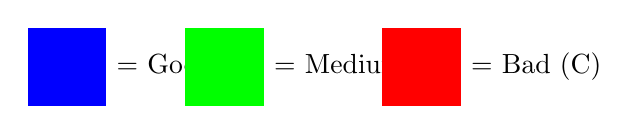
\begin{tikzpicture}
\node[inner sep=0pt] (r) at (0,0) {\tikz\fill[blue] (0,0) rectangle (\rectWidth,\rectHeight);};
\node[anchor=west] at (r.east) { = Good (A)};

\node[inner sep=0pt] (g) at (2,0) {\tikz\fill[green] (0,0) rectangle (\rectWidth,\rectHeight);};
\node[anchor=west] at (g.east) { = Medium (B)};

\node[inner sep=0pt] (b) at (4.5,0) {\tikz\fill[red] (0,0) rectangle (\rectWidth,\rectHeight);};
\node[anchor=west] at (b.east) { = Bad (C)};
\end{tikzpicture}
\vspace{2mm}

\caption{The poem orders obtained in evaluations by human non-expert judges, according to data from~\citet{lamb2015human}, where every poem is colour coded with its ground truth category.  In all cases, poems are shown in order from highest-rated to lowest-rated; the predominance of red-coded poems at the top of the highest human ratings for Typicality, for example, shows that humans' highest-scoring poems for that category tended to come from the lowest-quality category of poems according to the ground truth.}
\label{fig:ordering_human_only}
\end{figure*}
\begin{figure*}[!ht]
% Adjust the rectangles' width and height as needed
\newcommand{\rectWidth}{0.06} % Width in cm
\newcommand{\rectHeight}{0.3} % Height in cm
\small
\setlength{\tabcolsep}{4pt}
  \begin{tabular}{l|c}
    \hline
    Criterion & Ordering  \\

\hline
% GROUND TRUTH ORDER: \\[1mm]
{\textbf{GROUND TRUTH:}} & \coloredRectangle{blue}{\rectWidth}{\rectHeight} \coloredRectangle{blue}{\rectWidth}{\rectHeight} \coloredRectangle{blue}{\rectWidth}{\rectHeight} \coloredRectangle{blue}{\rectWidth}{\rectHeight} \coloredRectangle{blue}{\rectWidth}{\rectHeight} \coloredRectangle{blue}{\rectWidth}{\rectHeight} \coloredRectangle{blue}{\rectWidth}{\rectHeight} \coloredRectangle{blue}{\rectWidth}{\rectHeight} \coloredRectangle{blue}{\rectWidth}{\rectHeight} \coloredRectangle{blue}{\rectWidth}{\rectHeight} \coloredRectangle{blue}{\rectWidth}{\rectHeight} \coloredRectangle{blue}{\rectWidth}{\rectHeight} \coloredRectangle{blue}{\rectWidth}{\rectHeight} \coloredRectangle{blue}{\rectWidth}{\rectHeight} \coloredRectangle{blue}{\rectWidth}{\rectHeight} \coloredRectangle{blue}{\rectWidth}{\rectHeight} \coloredRectangle{blue}{\rectWidth}{\rectHeight} \coloredRectangle{blue}{\rectWidth}{\rectHeight} \coloredRectangle{blue}{\rectWidth}{\rectHeight} \coloredRectangle{blue}{\rectWidth}{\rectHeight} \coloredRectangle{blue}{\rectWidth}{\rectHeight} \coloredRectangle{blue}{\rectWidth}{\rectHeight} \coloredRectangle{blue}{\rectWidth}{\rectHeight} \coloredRectangle{blue}{\rectWidth}{\rectHeight} \coloredRectangle{blue}{\rectWidth}{\rectHeight} \coloredRectangle{blue}{\rectWidth}{\rectHeight} \coloredRectangle{blue}{\rectWidth}{\rectHeight} \coloredRectangle{blue}{\rectWidth}{\rectHeight} \coloredRectangle{blue}{\rectWidth}{\rectHeight} \coloredRectangle{blue}{\rectWidth}{\rectHeight} \coloredRectangle{green}{\rectWidth}{\rectHeight} \coloredRectangle{green}{\rectWidth}{\rectHeight} \coloredRectangle{green}{\rectWidth}{\rectHeight} \coloredRectangle{green}{\rectWidth}{\rectHeight} \coloredRectangle{green}{\rectWidth}{\rectHeight} \coloredRectangle{green}{\rectWidth}{\rectHeight} \coloredRectangle{green}{\rectWidth}{\rectHeight} \coloredRectangle{green}{\rectWidth}{\rectHeight} \coloredRectangle{green}{\rectWidth}{\rectHeight} \coloredRectangle{green}{\rectWidth}{\rectHeight} \coloredRectangle{green}{\rectWidth}{\rectHeight} \coloredRectangle{green}{\rectWidth}{\rectHeight} \coloredRectangle{green}{\rectWidth}{\rectHeight} \coloredRectangle{green}{\rectWidth}{\rectHeight} \coloredRectangle{green}{\rectWidth}{\rectHeight} \coloredRectangle{green}{\rectWidth}{\rectHeight} \coloredRectangle{green}{\rectWidth}{\rectHeight} \coloredRectangle{green}{\rectWidth}{\rectHeight} \coloredRectangle{green}{\rectWidth}{\rectHeight} \coloredRectangle{green}{\rectWidth}{\rectHeight} \coloredRectangle{green}{\rectWidth}{\rectHeight} \coloredRectangle{green}{\rectWidth}{\rectHeight} \coloredRectangle{green}{\rectWidth}{\rectHeight} \coloredRectangle{green}{\rectWidth}{\rectHeight} \coloredRectangle{green}{\rectWidth}{\rectHeight} \coloredRectangle{green}{\rectWidth}{\rectHeight} \coloredRectangle{green}{\rectWidth}{\rectHeight} \coloredRectangle{green}{\rectWidth}{\rectHeight} \coloredRectangle{green}{\rectWidth}{\rectHeight} \coloredRectangle{green}{\rectWidth}{\rectHeight} \coloredRectangle{red}{\rectWidth}{\rectHeight} \coloredRectangle{red}{\rectWidth}{\rectHeight} \coloredRectangle{red}{\rectWidth}{\rectHeight} \coloredRectangle{red}{\rectWidth}{\rectHeight} \coloredRectangle{red}{\rectWidth}{\rectHeight} \coloredRectangle{red}{\rectWidth}{\rectHeight} \coloredRectangle{red}{\rectWidth}{\rectHeight} \coloredRectangle{red}{\rectWidth}{\rectHeight} \coloredRectangle{red}{\rectWidth}{\rectHeight} \coloredRectangle{red}{\rectWidth}{\rectHeight} \coloredRectangle{red}{\rectWidth}{\rectHeight} \coloredRectangle{red}{\rectWidth}{\rectHeight} \coloredRectangle{red}{\rectWidth}{\rectHeight} \coloredRectangle{red}{\rectWidth}{\rectHeight} \coloredRectangle{red}{\rectWidth}{\rectHeight} \coloredRectangle{red}{\rectWidth}{\rectHeight} \coloredRectangle{red}{\rectWidth}{\rectHeight} \coloredRectangle{red}{\rectWidth}{\rectHeight} \coloredRectangle{red}{\rectWidth}{\rectHeight} \coloredRectangle{red}{\rectWidth}{\rectHeight} \coloredRectangle{red}{\rectWidth}{\rectHeight} \coloredRectangle{red}{\rectWidth}{\rectHeight} \coloredRectangle{red}{\rectWidth}{\rectHeight} \coloredRectangle{red}{\rectWidth}{\rectHeight} \coloredRectangle{red}{\rectWidth}{\rectHeight} \coloredRectangle{red}{\rectWidth}{\rectHeight} \coloredRectangle{red}{\rectWidth}{\rectHeight} \coloredRectangle{red}{\rectWidth}{\rectHeight} \coloredRectangle{red}{\rectWidth}{\rectHeight} \coloredRectangle{red}{\rectWidth}{\rectHeight}\\

\hline

% \vspace{1mm}

{\textbf{QUALITY:}} & \coloredRectangle{blue}{\rectWidth}{\rectHeight} \coloredRectangle{blue}{\rectWidth}{\rectHeight} \coloredRectangle{blue}{\rectWidth}{\rectHeight} \coloredRectangle{blue}{\rectWidth}{\rectHeight} \coloredRectangle{blue}{\rectWidth}{\rectHeight} \coloredRectangle{green}{\rectWidth}{\rectHeight} \coloredRectangle{green}{\rectWidth}{\rectHeight} \coloredRectangle{blue}{\rectWidth}{\rectHeight} \coloredRectangle{blue}{\rectWidth}{\rectHeight} \coloredRectangle{blue}{\rectWidth}{\rectHeight} \coloredRectangle{blue}{\rectWidth}{\rectHeight} \coloredRectangle{blue}{\rectWidth}{\rectHeight} \coloredRectangle{green}{\rectWidth}{\rectHeight} \coloredRectangle{blue}{\rectWidth}{\rectHeight} \coloredRectangle{blue}{\rectWidth}{\rectHeight} \coloredRectangle{green}{\rectWidth}{\rectHeight} \coloredRectangle{blue}{\rectWidth}{\rectHeight} \coloredRectangle{blue}{\rectWidth}{\rectHeight} \coloredRectangle{blue}{\rectWidth}{\rectHeight} \coloredRectangle{green}{\rectWidth}{\rectHeight} \coloredRectangle{blue}{\rectWidth}{\rectHeight} \coloredRectangle{blue}{\rectWidth}{\rectHeight} \coloredRectangle{blue}{\rectWidth}{\rectHeight} \coloredRectangle{blue}{\rectWidth}{\rectHeight} \coloredRectangle{blue}{\rectWidth}{\rectHeight} \coloredRectangle{blue}{\rectWidth}{\rectHeight} \coloredRectangle{blue}{\rectWidth}{\rectHeight} \coloredRectangle{blue}{\rectWidth}{\rectHeight} \coloredRectangle{blue}{\rectWidth}{\rectHeight} \coloredRectangle{green}{\rectWidth}{\rectHeight} \coloredRectangle{green}{\rectWidth}{\rectHeight} \coloredRectangle{green}{\rectWidth}{\rectHeight} \coloredRectangle{green}{\rectWidth}{\rectHeight} \coloredRectangle{green}{\rectWidth}{\rectHeight} \coloredRectangle{green}{\rectWidth}{\rectHeight} \coloredRectangle{green}{\rectWidth}{\rectHeight} \coloredRectangle{blue}{\rectWidth}{\rectHeight} \coloredRectangle{green}{\rectWidth}{\rectHeight} \coloredRectangle{green}{\rectWidth}{\rectHeight} \coloredRectangle{green}{\rectWidth}{\rectHeight} \coloredRectangle{green}{\rectWidth}{\rectHeight} \coloredRectangle{blue}{\rectWidth}{\rectHeight} \coloredRectangle{green}{\rectWidth}{\rectHeight} \coloredRectangle{green}{\rectWidth}{\rectHeight} \coloredRectangle{green}{\rectWidth}{\rectHeight} \coloredRectangle{green}{\rectWidth}{\rectHeight} \coloredRectangle{blue}{\rectWidth}{\rectHeight} \coloredRectangle{green}{\rectWidth}{\rectHeight} \coloredRectangle{green}{\rectWidth}{\rectHeight} \coloredRectangle{green}{\rectWidth}{\rectHeight} \coloredRectangle{red}{\rectWidth}{\rectHeight} \coloredRectangle{green}{\rectWidth}{\rectHeight} \coloredRectangle{blue}{\rectWidth}{\rectHeight} \coloredRectangle{green}{\rectWidth}{\rectHeight} \coloredRectangle{blue}{\rectWidth}{\rectHeight} \coloredRectangle{blue}{\rectWidth}{\rectHeight} \coloredRectangle{green}{\rectWidth}{\rectHeight} \coloredRectangle{red}{\rectWidth}{\rectHeight} \coloredRectangle{green}{\rectWidth}{\rectHeight} \coloredRectangle{green}{\rectWidth}{\rectHeight} \coloredRectangle{green}{\rectWidth}{\rectHeight} \coloredRectangle{red}{\rectWidth}{\rectHeight} \coloredRectangle{red}{\rectWidth}{\rectHeight} \coloredRectangle{green}{\rectWidth}{\rectHeight} \coloredRectangle{red}{\rectWidth}{\rectHeight} \coloredRectangle{red}{\rectWidth}{\rectHeight} \coloredRectangle{red}{\rectWidth}{\rectHeight} \coloredRectangle{red}{\rectWidth}{\rectHeight} \coloredRectangle{red}{\rectWidth}{\rectHeight} \coloredRectangle{red}{\rectWidth}{\rectHeight} \coloredRectangle{red}{\rectWidth}{\rectHeight} \coloredRectangle{red}{\rectWidth}{\rectHeight} \coloredRectangle{red}{\rectWidth}{\rectHeight} \coloredRectangle{red}{\rectWidth}{\rectHeight} \coloredRectangle{red}{\rectWidth}{\rectHeight} \coloredRectangle{red}{\rectWidth}{\rectHeight} \coloredRectangle{red}{\rectWidth}{\rectHeight} \coloredRectangle{red}{\rectWidth}{\rectHeight} \coloredRectangle{red}{\rectWidth}{\rectHeight} \coloredRectangle{red}{\rectWidth}{\rectHeight} \coloredRectangle{red}{\rectWidth}{\rectHeight} \coloredRectangle{red}{\rectWidth}{\rectHeight} \coloredRectangle{red}{\rectWidth}{\rectHeight} \coloredRectangle{red}{\rectWidth}{\rectHeight} \coloredRectangle{red}{\rectWidth}{\rectHeight} \coloredRectangle{red}{\rectWidth}{\rectHeight} \coloredRectangle{red}{\rectWidth}{\rectHeight} \coloredRectangle{red}{\rectWidth}{\rectHeight} \coloredRectangle{red}{\rectWidth}{\rectHeight} \coloredRectangle{red}{\rectWidth}{\rectHeight}\\

% \vspace{1mm}

{\textbf{INNOVATIVENESS:}} & \coloredRectangle{blue}{\rectWidth}{\rectHeight} \coloredRectangle{green}{\rectWidth}{\rectHeight} \coloredRectangle{blue}{\rectWidth}{\rectHeight} \coloredRectangle{green}{\rectWidth}{\rectHeight} \coloredRectangle{blue}{\rectWidth}{\rectHeight} \coloredRectangle{green}{\rectWidth}{\rectHeight} \coloredRectangle{blue}{\rectWidth}{\rectHeight} \coloredRectangle{blue}{\rectWidth}{\rectHeight} \coloredRectangle{blue}{\rectWidth}{\rectHeight} \coloredRectangle{green}{\rectWidth}{\rectHeight} \coloredRectangle{blue}{\rectWidth}{\rectHeight} \coloredRectangle{green}{\rectWidth}{\rectHeight} \coloredRectangle{blue}{\rectWidth}{\rectHeight} \coloredRectangle{blue}{\rectWidth}{\rectHeight} \coloredRectangle{blue}{\rectWidth}{\rectHeight} \coloredRectangle{green}{\rectWidth}{\rectHeight} \coloredRectangle{blue}{\rectWidth}{\rectHeight} \coloredRectangle{blue}{\rectWidth}{\rectHeight} \coloredRectangle{green}{\rectWidth}{\rectHeight} \coloredRectangle{green}{\rectWidth}{\rectHeight} \coloredRectangle{blue}{\rectWidth}{\rectHeight} \coloredRectangle{red}{\rectWidth}{\rectHeight} \coloredRectangle{blue}{\rectWidth}{\rectHeight} \coloredRectangle{blue}{\rectWidth}{\rectHeight} \coloredRectangle{green}{\rectWidth}{\rectHeight} \coloredRectangle{green}{\rectWidth}{\rectHeight} \coloredRectangle{blue}{\rectWidth}{\rectHeight} \coloredRectangle{blue}{\rectWidth}{\rectHeight} \coloredRectangle{blue}{\rectWidth}{\rectHeight} \coloredRectangle{green}{\rectWidth}{\rectHeight} \coloredRectangle{blue}{\rectWidth}{\rectHeight} \coloredRectangle{blue}{\rectWidth}{\rectHeight} \coloredRectangle{green}{\rectWidth}{\rectHeight} \coloredRectangle{blue}{\rectWidth}{\rectHeight} \coloredRectangle{green}{\rectWidth}{\rectHeight} \coloredRectangle{green}{\rectWidth}{\rectHeight} \coloredRectangle{green}{\rectWidth}{\rectHeight} \coloredRectangle{blue}{\rectWidth}{\rectHeight} \coloredRectangle{green}{\rectWidth}{\rectHeight} \coloredRectangle{green}{\rectWidth}{\rectHeight} \coloredRectangle{blue}{\rectWidth}{\rectHeight} \coloredRectangle{green}{\rectWidth}{\rectHeight} \coloredRectangle{green}{\rectWidth}{\rectHeight} \coloredRectangle{blue}{\rectWidth}{\rectHeight} \coloredRectangle{blue}{\rectWidth}{\rectHeight} \coloredRectangle{blue}{\rectWidth}{\rectHeight} \coloredRectangle{blue}{\rectWidth}{\rectHeight} \coloredRectangle{green}{\rectWidth}{\rectHeight} \coloredRectangle{blue}{\rectWidth}{\rectHeight} \coloredRectangle{red}{\rectWidth}{\rectHeight} \coloredRectangle{red}{\rectWidth}{\rectHeight} \coloredRectangle{blue}{\rectWidth}{\rectHeight} \coloredRectangle{blue}{\rectWidth}{\rectHeight} \coloredRectangle{green}{\rectWidth}{\rectHeight} \coloredRectangle{green}{\rectWidth}{\rectHeight} \coloredRectangle{green}{\rectWidth}{\rectHeight} \coloredRectangle{red}{\rectWidth}{\rectHeight} \coloredRectangle{green}{\rectWidth}{\rectHeight} \coloredRectangle{red}{\rectWidth}{\rectHeight} \coloredRectangle{green}{\rectWidth}{\rectHeight} \coloredRectangle{red}{\rectWidth}{\rectHeight} \coloredRectangle{red}{\rectWidth}{\rectHeight} \coloredRectangle{green}{\rectWidth}{\rectHeight} \coloredRectangle{red}{\rectWidth}{\rectHeight} \coloredRectangle{red}{\rectWidth}{\rectHeight} \coloredRectangle{green}{\rectWidth}{\rectHeight} \coloredRectangle{green}{\rectWidth}{\rectHeight} \coloredRectangle{red}{\rectWidth}{\rectHeight} \coloredRectangle{red}{\rectWidth}{\rectHeight} \coloredRectangle{red}{\rectWidth}{\rectHeight} \coloredRectangle{red}{\rectWidth}{\rectHeight} \coloredRectangle{red}{\rectWidth}{\rectHeight} \coloredRectangle{red}{\rectWidth}{\rectHeight} \coloredRectangle{green}{\rectWidth}{\rectHeight} \coloredRectangle{red}{\rectWidth}{\rectHeight} \coloredRectangle{red}{\rectWidth}{\rectHeight} \coloredRectangle{red}{\rectWidth}{\rectHeight} \coloredRectangle{green}{\rectWidth}{\rectHeight} \coloredRectangle{red}{\rectWidth}{\rectHeight} \coloredRectangle{red}{\rectWidth}{\rectHeight} \coloredRectangle{red}{\rectWidth}{\rectHeight} \coloredRectangle{red}{\rectWidth}{\rectHeight} \coloredRectangle{red}{\rectWidth}{\rectHeight} \coloredRectangle{red}{\rectWidth}{\rectHeight} \coloredRectangle{red}{\rectWidth}{\rectHeight} \coloredRectangle{red}{\rectWidth}{\rectHeight} \coloredRectangle{red}{\rectWidth}{\rectHeight} \coloredRectangle{red}{\rectWidth}{\rectHeight} \coloredRectangle{red}{\rectWidth}{\rectHeight} \coloredRectangle{red}{\rectWidth}{\rectHeight}\\


% \vspace{1mm}

{\textbf{CREATIVITY:}} & \coloredRectangle{blue}{\rectWidth}{\rectHeight} \coloredRectangle{green}{\rectWidth}{\rectHeight} \coloredRectangle{blue}{\rectWidth}{\rectHeight} \coloredRectangle{green}{\rectWidth}{\rectHeight} \coloredRectangle{blue}{\rectWidth}{\rectHeight} \coloredRectangle{blue}{\rectWidth}{\rectHeight} \coloredRectangle{green}{\rectWidth}{\rectHeight} \coloredRectangle{blue}{\rectWidth}{\rectHeight} \coloredRectangle{blue}{\rectWidth}{\rectHeight} \coloredRectangle{blue}{\rectWidth}{\rectHeight} \coloredRectangle{blue}{\rectWidth}{\rectHeight} \coloredRectangle{green}{\rectWidth}{\rectHeight} \coloredRectangle{blue}{\rectWidth}{\rectHeight} \coloredRectangle{blue}{\rectWidth}{\rectHeight} \coloredRectangle{blue}{\rectWidth}{\rectHeight} \coloredRectangle{green}{\rectWidth}{\rectHeight} \coloredRectangle{green}{\rectWidth}{\rectHeight} \coloredRectangle{blue}{\rectWidth}{\rectHeight} \coloredRectangle{red}{\rectWidth}{\rectHeight} \coloredRectangle{green}{\rectWidth}{\rectHeight} \coloredRectangle{blue}{\rectWidth}{\rectHeight} \coloredRectangle{blue}{\rectWidth}{\rectHeight} \coloredRectangle{blue}{\rectWidth}{\rectHeight} \coloredRectangle{green}{\rectWidth}{\rectHeight} \coloredRectangle{green}{\rectWidth}{\rectHeight} \coloredRectangle{blue}{\rectWidth}{\rectHeight} \coloredRectangle{blue}{\rectWidth}{\rectHeight} \coloredRectangle{green}{\rectWidth}{\rectHeight} \coloredRectangle{blue}{\rectWidth}{\rectHeight} \coloredRectangle{blue}{\rectWidth}{\rectHeight} \coloredRectangle{green}{\rectWidth}{\rectHeight} \coloredRectangle{blue}{\rectWidth}{\rectHeight} \coloredRectangle{green}{\rectWidth}{\rectHeight} \coloredRectangle{blue}{\rectWidth}{\rectHeight} \coloredRectangle{green}{\rectWidth}{\rectHeight} \coloredRectangle{blue}{\rectWidth}{\rectHeight} \coloredRectangle{blue}{\rectWidth}{\rectHeight} \coloredRectangle{blue}{\rectWidth}{\rectHeight} \coloredRectangle{green}{\rectWidth}{\rectHeight} \coloredRectangle{blue}{\rectWidth}{\rectHeight} \coloredRectangle{red}{\rectWidth}{\rectHeight} \coloredRectangle{blue}{\rectWidth}{\rectHeight} \coloredRectangle{green}{\rectWidth}{\rectHeight} \coloredRectangle{green}{\rectWidth}{\rectHeight} \coloredRectangle{blue}{\rectWidth}{\rectHeight} \coloredRectangle{green}{\rectWidth}{\rectHeight} \coloredRectangle{green}{\rectWidth}{\rectHeight} \coloredRectangle{blue}{\rectWidth}{\rectHeight} \coloredRectangle{green}{\rectWidth}{\rectHeight} \coloredRectangle{green}{\rectWidth}{\rectHeight} \coloredRectangle{green}{\rectWidth}{\rectHeight} \coloredRectangle{green}{\rectWidth}{\rectHeight} \coloredRectangle{blue}{\rectWidth}{\rectHeight} \coloredRectangle{green}{\rectWidth}{\rectHeight} \coloredRectangle{red}{\rectWidth}{\rectHeight} \coloredRectangle{red}{\rectWidth}{\rectHeight} \coloredRectangle{blue}{\rectWidth}{\rectHeight} \coloredRectangle{green}{\rectWidth}{\rectHeight} \coloredRectangle{green}{\rectWidth}{\rectHeight} \coloredRectangle{red}{\rectWidth}{\rectHeight} \coloredRectangle{green}{\rectWidth}{\rectHeight} \coloredRectangle{red}{\rectWidth}{\rectHeight} \coloredRectangle{red}{\rectWidth}{\rectHeight} \coloredRectangle{green}{\rectWidth}{\rectHeight} \coloredRectangle{red}{\rectWidth}{\rectHeight} \coloredRectangle{green}{\rectWidth}{\rectHeight} \coloredRectangle{green}{\rectWidth}{\rectHeight} \coloredRectangle{green}{\rectWidth}{\rectHeight} \coloredRectangle{red}{\rectWidth}{\rectHeight} \coloredRectangle{red}{\rectWidth}{\rectHeight} \coloredRectangle{red}{\rectWidth}{\rectHeight} \coloredRectangle{red}{\rectWidth}{\rectHeight} \coloredRectangle{red}{\rectWidth}{\rectHeight} \coloredRectangle{red}{\rectWidth}{\rectHeight} \coloredRectangle{red}{\rectWidth}{\rectHeight} \coloredRectangle{red}{\rectWidth}{\rectHeight} \coloredRectangle{red}{\rectWidth}{\rectHeight} \coloredRectangle{red}{\rectWidth}{\rectHeight} \coloredRectangle{red}{\rectWidth}{\rectHeight} \coloredRectangle{red}{\rectWidth}{\rectHeight} \coloredRectangle{red}{\rectWidth}{\rectHeight} \coloredRectangle{red}{\rectWidth}{\rectHeight} \coloredRectangle{red}{\rectWidth}{\rectHeight} \coloredRectangle{red}{\rectWidth}{\rectHeight} \coloredRectangle{red}{\rectWidth}{\rectHeight} \coloredRectangle{red}{\rectWidth}{\rectHeight} \coloredRectangle{red}{\rectWidth}{\rectHeight} \coloredRectangle{red}{\rectWidth}{\rectHeight} \coloredRectangle{red}{\rectWidth}{\rectHeight} \coloredRectangle{red}{\rectWidth}{\rectHeight}\\


% \vspace{1mm}

{\textbf{POETICNESS:}} & \coloredRectangle{blue}{\rectWidth}{\rectHeight} \coloredRectangle{blue}{\rectWidth}{\rectHeight} \coloredRectangle{blue}{\rectWidth}{\rectHeight} \coloredRectangle{blue}{\rectWidth}{\rectHeight} \coloredRectangle{green}{\rectWidth}{\rectHeight} \coloredRectangle{green}{\rectWidth}{\rectHeight} \coloredRectangle{blue}{\rectWidth}{\rectHeight} \coloredRectangle{blue}{\rectWidth}{\rectHeight} \coloredRectangle{blue}{\rectWidth}{\rectHeight} \coloredRectangle{blue}{\rectWidth}{\rectHeight} \coloredRectangle{blue}{\rectWidth}{\rectHeight} \coloredRectangle{green}{\rectWidth}{\rectHeight} \coloredRectangle{blue}{\rectWidth}{\rectHeight} \coloredRectangle{blue}{\rectWidth}{\rectHeight} \coloredRectangle{green}{\rectWidth}{\rectHeight} \coloredRectangle{blue}{\rectWidth}{\rectHeight} \coloredRectangle{blue}{\rectWidth}{\rectHeight} \coloredRectangle{green}{\rectWidth}{\rectHeight} \coloredRectangle{blue}{\rectWidth}{\rectHeight} \coloredRectangle{blue}{\rectWidth}{\rectHeight} \coloredRectangle{blue}{\rectWidth}{\rectHeight} \coloredRectangle{blue}{\rectWidth}{\rectHeight} \coloredRectangle{blue}{\rectWidth}{\rectHeight} \coloredRectangle{green}{\rectWidth}{\rectHeight} \coloredRectangle{green}{\rectWidth}{\rectHeight} \coloredRectangle{green}{\rectWidth}{\rectHeight} \coloredRectangle{blue}{\rectWidth}{\rectHeight} \coloredRectangle{blue}{\rectWidth}{\rectHeight} \coloredRectangle{blue}{\rectWidth}{\rectHeight} \coloredRectangle{blue}{\rectWidth}{\rectHeight} \coloredRectangle{blue}{\rectWidth}{\rectHeight} \coloredRectangle{green}{\rectWidth}{\rectHeight} \coloredRectangle{green}{\rectWidth}{\rectHeight} \coloredRectangle{green}{\rectWidth}{\rectHeight} \coloredRectangle{blue}{\rectWidth}{\rectHeight} \coloredRectangle{blue}{\rectWidth}{\rectHeight} \coloredRectangle{green}{\rectWidth}{\rectHeight} \coloredRectangle{green}{\rectWidth}{\rectHeight} \coloredRectangle{green}{\rectWidth}{\rectHeight} \coloredRectangle{green}{\rectWidth}{\rectHeight} \coloredRectangle{green}{\rectWidth}{\rectHeight} \coloredRectangle{green}{\rectWidth}{\rectHeight} \coloredRectangle{green}{\rectWidth}{\rectHeight} \coloredRectangle{blue}{\rectWidth}{\rectHeight} \coloredRectangle{green}{\rectWidth}{\rectHeight} \coloredRectangle{red}{\rectWidth}{\rectHeight} \coloredRectangle{blue}{\rectWidth}{\rectHeight} \coloredRectangle{green}{\rectWidth}{\rectHeight} \coloredRectangle{blue}{\rectWidth}{\rectHeight} \coloredRectangle{red}{\rectWidth}{\rectHeight} \coloredRectangle{green}{\rectWidth}{\rectHeight} \coloredRectangle{blue}{\rectWidth}{\rectHeight} \coloredRectangle{green}{\rectWidth}{\rectHeight} \coloredRectangle{green}{\rectWidth}{\rectHeight} \coloredRectangle{blue}{\rectWidth}{\rectHeight} \coloredRectangle{red}{\rectWidth}{\rectHeight} \coloredRectangle{green}{\rectWidth}{\rectHeight} \coloredRectangle{red}{\rectWidth}{\rectHeight} \coloredRectangle{green}{\rectWidth}{\rectHeight} \coloredRectangle{green}{\rectWidth}{\rectHeight} \coloredRectangle{green}{\rectWidth}{\rectHeight} \coloredRectangle{red}{\rectWidth}{\rectHeight} \coloredRectangle{red}{\rectWidth}{\rectHeight} \coloredRectangle{red}{\rectWidth}{\rectHeight} \coloredRectangle{red}{\rectWidth}{\rectHeight} \coloredRectangle{red}{\rectWidth}{\rectHeight} \coloredRectangle{red}{\rectWidth}{\rectHeight} \coloredRectangle{green}{\rectWidth}{\rectHeight} \coloredRectangle{green}{\rectWidth}{\rectHeight} \coloredRectangle{red}{\rectWidth}{\rectHeight} \coloredRectangle{red}{\rectWidth}{\rectHeight} \coloredRectangle{red}{\rectWidth}{\rectHeight} \coloredRectangle{red}{\rectWidth}{\rectHeight} \coloredRectangle{green}{\rectWidth}{\rectHeight} \coloredRectangle{red}{\rectWidth}{\rectHeight} \coloredRectangle{red}{\rectWidth}{\rectHeight} \coloredRectangle{red}{\rectWidth}{\rectHeight} \coloredRectangle{red}{\rectWidth}{\rectHeight} \coloredRectangle{red}{\rectWidth}{\rectHeight} \coloredRectangle{red}{\rectWidth}{\rectHeight} \coloredRectangle{red}{\rectWidth}{\rectHeight} \coloredRectangle{red}{\rectWidth}{\rectHeight} \coloredRectangle{red}{\rectWidth}{\rectHeight} \coloredRectangle{red}{\rectWidth}{\rectHeight} \coloredRectangle{red}{\rectWidth}{\rectHeight} \coloredRectangle{red}{\rectWidth}{\rectHeight} \coloredRectangle{red}{\rectWidth}{\rectHeight} \coloredRectangle{red}{\rectWidth}{\rectHeight} \coloredRectangle{red}{\rectWidth}{\rectHeight} \coloredRectangle{red}{\rectWidth}{\rectHeight}\\

 % \vspace{1mm}
   
{\textbf{SIMILARITY:}} & \coloredRectangle{blue}{\rectWidth}{\rectHeight} \coloredRectangle{green}{\rectWidth}{\rectHeight} \coloredRectangle{blue}{\rectWidth}{\rectHeight} \coloredRectangle{blue}{\rectWidth}{\rectHeight} \coloredRectangle{blue}{\rectWidth}{\rectHeight} \coloredRectangle{green}{\rectWidth}{\rectHeight} \coloredRectangle{blue}{\rectWidth}{\rectHeight} \coloredRectangle{blue}{\rectWidth}{\rectHeight} \coloredRectangle{blue}{\rectWidth}{\rectHeight} \coloredRectangle{blue}{\rectWidth}{\rectHeight} \coloredRectangle{green}{\rectWidth}{\rectHeight} \coloredRectangle{blue}{\rectWidth}{\rectHeight} \coloredRectangle{blue}{\rectWidth}{\rectHeight} \coloredRectangle{green}{\rectWidth}{\rectHeight} \coloredRectangle{blue}{\rectWidth}{\rectHeight} \coloredRectangle{blue}{\rectWidth}{\rectHeight} \coloredRectangle{blue}{\rectWidth}{\rectHeight} \coloredRectangle{blue}{\rectWidth}{\rectHeight} \coloredRectangle{blue}{\rectWidth}{\rectHeight} \coloredRectangle{blue}{\rectWidth}{\rectHeight} \coloredRectangle{blue}{\rectWidth}{\rectHeight} \coloredRectangle{green}{\rectWidth}{\rectHeight} \coloredRectangle{blue}{\rectWidth}{\rectHeight} \coloredRectangle{blue}{\rectWidth}{\rectHeight} \coloredRectangle{blue}{\rectWidth}{\rectHeight} \coloredRectangle{blue}{\rectWidth}{\rectHeight} \coloredRectangle{green}{\rectWidth}{\rectHeight} \coloredRectangle{blue}{\rectWidth}{\rectHeight} \coloredRectangle{blue}{\rectWidth}{\rectHeight} \coloredRectangle{blue}{\rectWidth}{\rectHeight} \coloredRectangle{blue}{\rectWidth}{\rectHeight} \coloredRectangle{green}{\rectWidth}{\rectHeight} \coloredRectangle{green}{\rectWidth}{\rectHeight} \coloredRectangle{green}{\rectWidth}{\rectHeight} \coloredRectangle{green}{\rectWidth}{\rectHeight} \coloredRectangle{blue}{\rectWidth}{\rectHeight} \coloredRectangle{green}{\rectWidth}{\rectHeight} \coloredRectangle{blue}{\rectWidth}{\rectHeight} \coloredRectangle{green}{\rectWidth}{\rectHeight} \coloredRectangle{blue}{\rectWidth}{\rectHeight} \coloredRectangle{green}{\rectWidth}{\rectHeight} \coloredRectangle{green}{\rectWidth}{\rectHeight} \coloredRectangle{green}{\rectWidth}{\rectHeight} \coloredRectangle{green}{\rectWidth}{\rectHeight} \coloredRectangle{green}{\rectWidth}{\rectHeight} \coloredRectangle{blue}{\rectWidth}{\rectHeight} \coloredRectangle{green}{\rectWidth}{\rectHeight} \coloredRectangle{blue}{\rectWidth}{\rectHeight} \coloredRectangle{green}{\rectWidth}{\rectHeight} \coloredRectangle{red}{\rectWidth}{\rectHeight} \coloredRectangle{green}{\rectWidth}{\rectHeight} \coloredRectangle{green}{\rectWidth}{\rectHeight} \coloredRectangle{red}{\rectWidth}{\rectHeight} \coloredRectangle{green}{\rectWidth}{\rectHeight} \coloredRectangle{red}{\rectWidth}{\rectHeight} \coloredRectangle{red}{\rectWidth}{\rectHeight} \coloredRectangle{green}{\rectWidth}{\rectHeight} \coloredRectangle{green}{\rectWidth}{\rectHeight} \coloredRectangle{green}{\rectWidth}{\rectHeight} \coloredRectangle{green}{\rectWidth}{\rectHeight} \coloredRectangle{red}{\rectWidth}{\rectHeight} \coloredRectangle{green}{\rectWidth}{\rectHeight} \coloredRectangle{green}{\rectWidth}{\rectHeight} \coloredRectangle{red}{\rectWidth}{\rectHeight} \coloredRectangle{green}{\rectWidth}{\rectHeight} \coloredRectangle{red}{\rectWidth}{\rectHeight} \coloredRectangle{red}{\rectWidth}{\rectHeight} \coloredRectangle{red}{\rectWidth}{\rectHeight} \coloredRectangle{red}{\rectWidth}{\rectHeight} \coloredRectangle{red}{\rectWidth}{\rectHeight} \coloredRectangle{red}{\rectWidth}{\rectHeight} \coloredRectangle{red}{\rectWidth}{\rectHeight} \coloredRectangle{green}{\rectWidth}{\rectHeight} \coloredRectangle{red}{\rectWidth}{\rectHeight} \coloredRectangle{red}{\rectWidth}{\rectHeight} \coloredRectangle{red}{\rectWidth}{\rectHeight} \coloredRectangle{red}{\rectWidth}{\rectHeight} \coloredRectangle{red}{\rectWidth}{\rectHeight} \coloredRectangle{red}{\rectWidth}{\rectHeight} \coloredRectangle{red}{\rectWidth}{\rectHeight} \coloredRectangle{red}{\rectWidth}{\rectHeight} \coloredRectangle{red}{\rectWidth}{\rectHeight} \coloredRectangle{red}{\rectWidth}{\rectHeight} \coloredRectangle{red}{\rectWidth}{\rectHeight} \coloredRectangle{red}{\rectWidth}{\rectHeight} \coloredRectangle{red}{\rectWidth}{\rectHeight} \coloredRectangle{red}{\rectWidth}{\rectHeight} \coloredRectangle{red}{\rectWidth}{\rectHeight} \coloredRectangle{red}{\rectWidth}{\rectHeight} \coloredRectangle{red}{\rectWidth}{\rectHeight}\\

 \hline


% \vspace{2mm}

% \hline
\end{tabular}

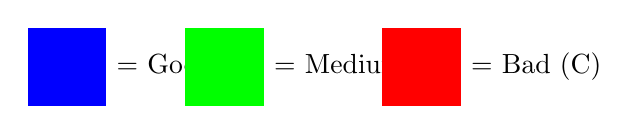
\begin{tikzpicture}
\node[inner sep=0pt] (r) at (0,0) {\tikz\fill[blue] (0,0) rectangle (\rectWidth,\rectHeight);};
\node[anchor=west] at (r.east) { = Good (A)};

\node[inner sep=0pt] (g) at (2,0) {\tikz\fill[green] (0,0) rectangle (\rectWidth,\rectHeight);};
\node[anchor=west] at (g.east) { = Medium (B)};

\node[inner sep=0pt] (b) at (4.5,0) {\tikz\fill[red] (0,0) rectangle (\rectWidth,\rectHeight);};
\node[anchor=west] at (b.east) { = Bad (C)};
\end{tikzpicture}

\caption{The poem orders determined by Claude-3--Opus 15n on all criteria, where every poem is colour coded with its ground truth category. This data come from Experiment 2, in Section \ref{subsection:Experiment 2}.}
\label{fig:ordering_claude15n}
\end{figure*}

\section{In-context Poem Evaluation} \label{secion:In Context}

We first explain how our prompts (Appendix~\ref{section:5_criteria_prompts}) for in-context evaluation ``force'' the LLMs towards comparative assessments. To this end, the prompts ask the LLMs to evaluate every poem in a set on a scale $1-5$, as these values worked best in our exploratory experiments. Additionally, the prompts (Appendix~\ref{section:5_criteria_prompts}) ask the LLMs to return the ordered list of poems. This second requirement brings us closer to the forced-choice methods \cite{brown2018modelling}. These two requirements in the prompts afford two scoring methods based on the same LLM outputs:
\begin{enumerate}
    \item Evaluations extracted from the $1-5$ scores will be referred to as Claude-3-Opus 90, Claude-3-Opus 15 and GPT-4o 15, where numbers \textit{90} and \textit{15} indicate the number of poems in a prompt.
    \item The poem's rank in the LLM's output list can be used as a score, where the first poem receives a score of 15, the second 14, and so on, until the last poem receives a score of 1. Evaluations done it this way will be referred to as Claude-3-Opus 90n, Claude-3-Opus 15n and GPT-4o 15n, where numbers \textit{90} and \textit{15} indicate the number of poems in a prompt.
\end{enumerate}
Note that the two scoring methods presented above yield the same order for one set of poems because they are part of the same output. However, when the averaged poem scores over 100 sets are computed, the two methods induce different orderings of the poems.

\subsection{Analyzing Input Size for In-context Poem Evaluation} \label{subsection:Analyzing Input Size}

Claude-3-Opus can analyze all 90 poems in a single prompt. On average 4 out of 5 such attempts were successful (i.e. the ranking of all 90 poems is provided in the response). Unsuccessful responses contained an incomplete list of poems, or contained duplicates, or, rarely, the LLM responded that it is incapable of fulfilling this task. 

For GPT-4o, only 3 out of 20 attempts to rank 90 poems were successful. This could be because of the phenomenon observed in~\citet{liu2024lost}--


\begin{table*}[ht]
\begin{center}
{
\small
\setlength{\tabcolsep}{5pt}
\begin{tabular}{ l||c|c|c|c|c|c|c|c|c|c|c|c }
\hline

\textbf{Criterion}  &\multicolumn{2}{c|}{\textbf{Claude-3 90n}} &\multicolumn{2}{c|}{\textbf{Claude-3 90}} &\multicolumn{2}{c|}{\textbf{Claude-3 15n}} &\multicolumn{2}{c|}{\textbf{Claude-3 15}} &\multicolumn{2}{c|}{\textbf{GPT-4o 15n}} &\multicolumn{2}{c}{\textbf{GPT-4o 15}} \\
\cline{2-13}
     &\textbf{SRC} &\textbf{p-val} &\textbf{SRC} &\textbf{p-val} &\textbf{SRC} &\textbf{p-val} &\textbf{SRC} &\textbf{p-val} &\textbf{SRC} &\textbf{p-val} &\textbf{SRC} &\textbf{p-val} \\

Innovative & 0.63 & 2.1e-11 & \textbf{0.68} & 1.2e-13 & 0.7 & 1.6e-14 & 0.67 & 7.4e-13 & 0.75 & 1.8e-17 & 0.73 & 2e-16 \\
Poeticness &  \textbf{0.67} & 7.36e-13 & 0.63 & 2.1e-11 & 0.8 & 3.2e-21 & 0.78 & 7.2e-20 & 0.68 & 1.2e-13 & 0.7 & 1.6e-14 \\
Creativity & 0.63 & 2.1e-11 & 0.62 & 9.7e-11 & 0.72 & 2e-15 & 0.68 & 1.2e-13 & 0.72 & 2e-15 & \textbf{0.77} & 1.3e-18 \\
Quality & 0.57 & 5.8e-09 & 0.57 & 5.8e-09 & \textbf{0.87} & 2.6e-28 & \textbf{0.85} & 3.2e-26 & \textbf{0.82} & 1e-22 & \textbf{0.77} & 1.3e-18 \\
Similarity & 0.47 & 3.5e-06 & 0.52 & 1.9e-07 & 0.83 & 2.2e-24 & 0.8 & 3.2e-21 & 0.7 & 1.6e-14 & 0.72 & 2e-15 \\
\end{tabular}
}
\end{center}
\caption{Results of Spearman's Rank Correlation (SRC) against the ground truth of the poems ordering in 5 criteria from 90-poems prompts using Claude-3-Opus (Experiment 2, ``Claude-3-Opus 90n'' and ``Claude-3-Opus 90'') and 15-poems prompts (Experiment 3, ``Claude-3-Opus 15'', ``Claude-3-Opus'', ``GPT-4o 15n'' and ``GPT-4o''). For comparison with human evaluations please see Table~\ref{tbl:human_results}.}
\label{tbl:exp_1_90_correlations}
\end{table*}


---while LLMs are capable of accepting very large prompts, the performance decreases with the length of the prompt, and the models do not handle equally well the whole content of the prompt. As a result, we reduced the GPT-4o input to 30 poems per prompt, resulting in a successful analysis in 17 out of 20 attempts. Further reduction to 15 poems per prompt increased the success rate to 100\%. Claude-3-Opus also successfully ranked the 15-poem prompts on every attempt.

Therefore, we will present the evaluations of 90 poems in one prompt for Claude-3-Opus only, and evaluations relying on 15 poems in one prompt for both Claude-3-Opus and GPT-4o.

\subsection{Experiment 2---Evaluation of Poems---90 poems in a prompt} \label{subsection:Experiment 2}

Since the GPT-4o version used in this study was incapable of evaluating all 90 poems in a single prompt, this experiment is conducted only with Claude-3-Opus. For prompts, we have prepared 10 datasets containing all 90 poems, where the poems' ordering for each dataset was randomized. Thus, each poem will be evaluated ten times.

Each of the ten 90-poem datasets underwent evaluation in the specified five criteria: Creativity, Quality, Innovativeness, Similarity, and Poeticness, using the prompts presented in Appendix~\ref{section:5_criteria_prompts}. Post-evaluation, the numerical scores for each poem were averaged, and the poems were ranked based on their average scores. We have used both the original 1--5 scale scores assigned by the model (Claude-3-Opus 90), and the poem's positions on the list (Claude-3-Opus 90n).

After sorting the poems by their average evaluation score, each poem's position was marked with the category it represents (A, B or C), thus producing an ordered list of A's, B's and C's. These lists were then compared to the ground truth, and  Spearman’s rank correlation was computed, using the ranks A, B, and C. Table~\ref{tbl:exp_1_90_correlations} presents Spearman's correlation coefficients calculated against the ground truth order, and Figure~\ref{fig:ordering_all4_human} (Appendix) presents graphical representations of the results. These outcomes demonstrate an even higher degree of correlation with the ground truth (SRC=0.68) as compared to ``without-context'' evaluations, and are all statistically significant, with very low p-values in every case. However, we note that some of the 90-poem evaluations failed and had to be repeated. Subsequent experiments will show that reducing the number of poems in the prompt improves the accuracy even further.


\subsection{Experiment 3---Evaluation of Poems---15 poems in a prompt}
\label{subsection:Experiment 3}


In this experiment, 5 poems were randomly selected from each category (A, B and C) to form a subset of 15 poems for each query to both LLMs. This process was repeated to create 100 unique subsets, each containing poems from all three categories and shuffled accordingly. 

Each of the 100 15-poem datasets underwent evaluation using the same five criteria: Creativity, Quality, Innovativeness, Similarity, and Poeticness, using the prompts shown in Appendix~\ref{section:5_criteria_prompts}.

Due to sampling, the frequency of poems across the 100 subsets was slightly different. After evaluation, scores for each poem were averaged across all subsets where they appeared, and the poems were ranked by their average evaluation scores. This was done for both types of scoring methods.

As before, each poem's position in the scoring list was marked with its category (A, B or C), resulting in an ordered list. These lists were compared to the ground truth using Spearman’s rank correlation with ranks A, B and C. Table~\ref{tbl:exp_1_90_correlations} presents those correlations, showing a very high degree of consistency with the ground truth, and all values are statistically significant with extremely low p-values.

Overall, most results surpass those obtained by Claude-3-Opus when evaluating all 90 poems in a single prompt and significantly surpass those of human non-expert judges. Evaluations of 15 poems per prompt yielded much higher correlations to the ground truth. The highest correlation, 0.87, was achieved in the Quality criterion by Claude-3-Opus (Table~\ref{tbl:exp_1_90_correlations} and Figure~\ref{fig:ordering_claude15n}) and  when the scores were the poem's positions in the list. For GPT-4o, the results were slightly lower, but the Quality criterion also yielded the highest correlation when the scores were the poem's positions in the list. Deriving the scores from the poem's positions consistently improved results for Claude-3-Opus, but this was not always true for GPT-4o (Table~\ref{tbl:exp_1_90_correlations} and Figure~\ref{fig:ordering_all4_human} in the Appendix).  

\begin{table}[]
\begin{center}
\small
\setlength{\tabcolsep}{4pt}
{
\begin{tabular}{ l|c|c|c|c|l }
\hline
\textbf{Criterion}& \textbf{Good} & \textbf{Medium} & \textbf{Bad} & \textbf{F-value} &\textbf{p-value} \\

\hline
Innovative& 10.83 & 9.02 & 4.26 & 52.89 & 9.3e-16 \\
Quality & 11.65 & 9.06 & 3.33 & 132.23  & 4.2e-27 \\
Creativity  & 11.11 & 8.95 & 4.02 & 62.55 & 1.46e-17\\
Poeticness& 11.42 & 8.81 & 3.79 & 85.15 & 3.27e-21 \\
Similarity  & 11.22 & 8.63 & 4.13 & 111.08 & 1.11e-24 \\
\end{tabular}
}
\end{center}
\caption{ANOVA results  for poem evaluation in five criteria in Experiment 3 for Claude-3-Opus 15n. Columns ``Good,'' ``Medium,'' and ``Bad'' present averaged scores for those poems' categories.}\label{tbl:var_1_results}
\end{table}

\subsubsection{Analysis of Variance}

Similar to the approach taken by \citet{lamb2015human}, we conducted a single-factor ANOVA for each evaluation criterion to compare the average scores of the ``Good,'' ``Medium,'' and ``Bad'' poem categories, as shown in Table~\ref{tbl:var_1_results} for Claude-3-Opus 15n and for all four evaluations, plus the evaluation of the results from Experiment~\ref{subsection:Experiment 2}, in Table~\ref{tbl:var_1_results_full} in the Appendix. Given that we had five evaluation criteria, we performed five separate ANOVAs for each model. The null hypothesis stated that all poem categories have the same population mean, while the alternative hypothesis suggested that significant differences exist among these means.

The results, presented in Table~\ref{tbl:var_1_results} and Table  \ref{tbl:var_1_results_full} (Appendix), indicate statistically significant differences between the poem category means for each criterion, considering the Bonferroni-corrected alpha level of 0.01. This finding implies that there are significant variations among the groups for all tested criteria, suggesting that a poem's category has a measurable impact on the scores of all five criteria.

We can also observe that using the poem's position in the output list as a scoring method increases the F-value and decreases the p-value in every case, indicating higher effect size of this approach.

\section{Experiment 4---Evaluating Poetry - Interrater Reliability of Claude-3-Opus and GPT-4o} \label{subsection:Experiment 4}

The primary goal of the previous experiments was to approximate the ground truth categorization. Now, we will test if the LLMs return different rankings when the same set-up is repeated several times (the LLM's temperature parameter was set to 1 to maximize randomness in all our experiments in this paper). After that, we check if the diverse outputs are consistent and reliable with respect to the rankings they yield. For that we conducted a dedicated experiment where we have randomly selected 1 subset of 15 poems (from the subsets used in Experiment 3) and evaluated this subset 10 times with our LLMs. We are evaluating both models with both scoring methods. Effectively, 200 evaluations were conducted (2 models $\times$ 2 ways of scoring  $\times$ 10 repetitions $\times$ 5 criteria).

In Table~\ref{tab:poetry_scores_example_iccc} (Appendix) we present an example of evaluating the ``Creativity'' criterion with Claude-3-Opus 15n and Claude-3-Opus, where the outputs are different, yet similar, across multiple runs of the same set-up.

Knowing that the outputs are diverse, we gauged the reliability of these LLM-based evaluations, and explored a range of Intraclass Correlation Coefficient (ICC) algorithms \cite{shrout1979intraclass}. We considered ICC models that cater to single measurements with fixed rater effects (ICC1), models treating raters as random effects from a larger pool (ICC2), and those considering systematic differences between raters (ICC3), along with their k-rater variants for average ratings. Given the experimental design leveraging repeated LLM queries, and reliance on the averaged scores, the ``k'' versions of the tests seem the most appropriate reliability measures, however in Table~\ref{tab:ICC_full} (Appendix) we present the results for all ICC evaluations.

The correlation results of ICC1k, ICC2k and ICC3k were all very similar, and they ranged between 0.9 and 0.99 for evaluations of in all 5 criteria. In every case, using the scores derived from the poem's position in the output list has significantly lowered the p-values and increased the F-scores. 

All ICCk tests show very high correlation between raters and all results are statistically significant because the p-values are very low. 

Overall, these results confirm that while the temperature parameter successfully diversifies the output of LLMs (Table~\ref{tab:poetry_scores_example_iccc}), the ICC results show that those diversified outputs are stable and reliable on average (Table~\ref{tab:ICC_full} in the Appendix).

\section{Comparing Claude-3-Opus and GPT-4o to Human Evaluations---Discussion} 


The progression of LLM performance in poetry evaluation demonstrates a clear superiority over non-expert human judges across multiple experiments.

In the without-context evaluation (Experiment 1), both Claude-3-Opus and GPT-4o already surpassed human performance, achieving correlations of 0.57 and 0.62 respectively. This improvement was achieved despite the models' tendency toward uneven distribution of categories, particularly their bias toward middle-category assignments. The progression of GPT-4 versions showed steady improvement, with the latest GPT-4o demonstrating the strongest correlation with ground truth.

The transition to in-context evaluations yielded even more substantial improvements. When evaluating 90 poems simultaneously, Claude-3-Opus achieved correlations ranging from 0.47 to 0.67, depending on the criterion and scoring method. These results consistently outperformed the human baseline across all evaluation criteria. The most significant improvements emerged in Experiment 3, where both models evaluated 15-poem subsets. Claude-3-Opus achieved its highest correlation of 0.87 for the ``Quality'' criterion, while GPT-4o reached 0.82, both substantially exceeding human performance.

The high reliability of LLM evaluations is further evidenced by the very high interrater reliability results from Experiment 4. Both Claude-3-Opus and GPT-4o demonstrated high ICC values ranging between 0.9 and 0.99 across all five evaluation criteria, with statistically significant p-values. These ICC scores, which exceed the typical acceptable threshold of 0.7-0.9 for human judges in CAT studies, indicate that despite the temperature parameter introducing variability in the models' outputs, their evaluations remain highly consistent and reliable across multiple iterations. This level of reliability suggests that LLMs can provide stable and reproducible poetry assessments, addressing one of the key challenges in creative evaluation - the need for consistent judgment across multiple evaluations.

These findings demonstrate that LLMs have already achieved remarkable capabilities in poetry evaluation with a meaningful understanding of poetic quality, consistently surpassing non-expert human judges across multiple criteria and experimental conditions. The combination of strong ground truth correlation and high inter-rater reliability across different evaluation methods validates their potential for reliable creative assessment.


\section{Conclusion} \label{section:Conclusion}


Our experiments highlight the potential of Large Language Models, specifically Claude-3-Opus and GPT-4o, to evaluate poetry, showing strong correlations with ground truth and outperforming non-expert human judges in ranking the poems. High inter-rater reliability across evaluation criteria underscores the models' consistency and robustness.

Our study contributes several technical insights into creative assessment using LLMs:

1. Novel Evaluation Method: We introduce a new evaluation methodology inspired by the Consensual Assessment Technique (CAT), showing that LLMs can provide consistent, reliable assessments across several criteria.

2. Optimized Data Evaluation: Evaluating smaller object sets yields better results than assessing entire datasets in one prompt, suggesting curated input data enhances assessment accuracy and reliability.

3. Scoring Methodology: The method of score computation significantly affects the results in poetry evaluation. Scores derived from a poem’s position in output lists yield higher correlations with ground truth and lower p-values than raw numerical scores.

Future work should explore these methods' scalability to larger datasets and refine prompts and criteria. While our study focused on comparison with non-expert evaluators, future research could explore how these models perform against expert human judges in professional contexts such as poetry competitions or editorial decision-making. As LLM capabilities grow, their role in the arts and humanities is set to expand. This study lays the groundwork for future research on the automated evaluation of creative works, which lies at the intersection of AI and human creativity, potentially leading to practical applications in literary evaluation and publishing.


\newpage

\bibliography{custom}

\clearpage
\onecolumn
%\appendix
\section{Appendix} \label{section:appendix}

\subsection{Prompts for Claude-3-Opus and GPT-4o poetry evaluation using 5 individual criteria.} \label{section:5_criteria_prompts}

\vspace{10pt}
CREATIVITY: Below is the collection of 15 (90) poems. Evaluate the creativity level of each poem on the scale from 1 to 5, with 1 being "least creative" and 5 being "most creative". Use the whole range of the scale, that is, the least creative poem in the collection must have the score of 1, and the most creative poem in the collection must have the score of 5. Use only whole integers without any decimal places. Print out the filenames of the poems with their associated scores, ordered from the highest score to the lowest, in the following format:

\vspace{10pt}

QUALITY: Below is a collection of 15 (90) poems. Evaluate the quality of each poem on a scale from 1 to 5, with 1 being "lowest quality" and 5 being "highest quality". Use the full range of the scale, meaning the lowest quality poem in the collection must receive a score of 1, and the highest quality poem must receive a score of 5. Use only whole integers without any decimal places. Print out the filenames of the poems with their associated scores, ordered from the highest score to the lowest, in the following format:

\vspace{10pt}

INNOVATIVENESS: Below is a collection of 15 (90) poems. Assess each text based on its innovativeness, using a scale from 1 to 5, with 1 indicating "This poem is like other poems I have seen before," and 5 indicating "This poem is not like other poems I have seen before." Utilize the entire scale, which means the poem from the collection that is least innovative should receive a score of 1, and the poem in the collection that most innovative should receive a score of 5. Use only whole integers without any decimal places. Print out the filenames of the poems with their associated scores, ordered from the highest score to the lowest, in the following format:

\vspace{10pt}

SIMILARITY: Below is a collection of 15 (90) poems. Assess each poem based on its similarity to other poems you have read, using a scale from 1 to 5, with 1 indicating "not at all similar" and 5 indicating "highly similar." Utilize the entire scale, which means the poem from the collection that is least similar to other poems you have readshould receive a score of 1, and the poem in the collection that most closely resembles other poems that you have read should receive a score of 5. Use only whole integers without any decimal places. Print out the filenames of the poems with their associated scores, ordered from the highest score to the lowest, in the following format:

\vspace{10pt}

POETICNESS: Below is a collection of 15 (90) texts. Assess each text based on its qualification as a poem, using a scale from 1 to 5, with 1 indicating "this is not a poem" and 5 indicating "this is definitely a poem." Utilize the entire scale, which means the text from the collection that least qualifies as a poem should receive a score of 1, and the text in the collection that most convincingly represents a poem should receive a score of 5. Use only whole integers without any decimal places. Print out the filenames of the poems with their associated scores,
ordered from the highest score to the lowest, in the following format:

[position on the list]. [poems author] -  [poems title] : [score]

below are two example entries:

1. Tom Smith - Some Poem : 5

2. Jane Jones - My Poem : 4

POEMS:

===========================



\subsection{Prompt for classifying the poem into one of the three categories without context.} \label{section:GPT3-ABC}


You will be evaluating poems and categorizing them as ``Good'', ``Medium'', or ``Bad'' based on the following criteria:

- ``Good'' poems are those that would be published in  the foremost English language poetry journal globally. These poems have been subjected to meticulous scrutiny by the magazine's editorial team.

- ``Medium'' poems are those that would be published in intermediate poetry magazines offering \$5-\$10 per poem. These poems have undergone some degree of editorial review.

- ``Bad'' poems are those that would be posted on the website for amateur poets, and would receive no positive feedback. This website does not have any editorial filtration.

Here is the poem to evaluate:

\textless{}poem\textgreater{}

...

\textless{}/poem\textgreater{}

Carefully read the poem and consider which category it belongs to based on the criteria above. Write your reasoning for the categorization inside \textless{}reasoning\textgreater{} tags. Then, output the final category you believe the poem belongs to inside \textless{}category\textgreater{} tags.


\begin{figure*}[!ht]
% Adjust the rectangles' width and height as needed
\newcommand{\rectWidth}{0.06} % Width in cm
\newcommand{\rectHeight}{0.3} % Height in cm
\small
\setlength{\tabcolsep}{4pt}
  \begin{tabular}{l|c}
    \hline
    Model & Ordering  \\
     \hline

& \multicolumn{1}{c}{\textbf{GROUND TRUTH ORDER}} \\
\hline
% GROUND TRUTH ORDER: \\[1mm]
&\coloredRectangle{blue}{\rectWidth}{\rectHeight} \coloredRectangle{blue}{\rectWidth}{\rectHeight} \coloredRectangle{blue}{\rectWidth}{\rectHeight} \coloredRectangle{blue}{\rectWidth}{\rectHeight} \coloredRectangle{blue}{\rectWidth}{\rectHeight} \coloredRectangle{blue}{\rectWidth}{\rectHeight} \coloredRectangle{blue}{\rectWidth}{\rectHeight} \coloredRectangle{blue}{\rectWidth}{\rectHeight} \coloredRectangle{blue}{\rectWidth}{\rectHeight} \coloredRectangle{blue}{\rectWidth}{\rectHeight} \coloredRectangle{blue}{\rectWidth}{\rectHeight} \coloredRectangle{blue}{\rectWidth}{\rectHeight} \coloredRectangle{blue}{\rectWidth}{\rectHeight} \coloredRectangle{blue}{\rectWidth}{\rectHeight} \coloredRectangle{blue}{\rectWidth}{\rectHeight} \coloredRectangle{blue}{\rectWidth}{\rectHeight} \coloredRectangle{blue}{\rectWidth}{\rectHeight} \coloredRectangle{blue}{\rectWidth}{\rectHeight} \coloredRectangle{blue}{\rectWidth}{\rectHeight} \coloredRectangle{blue}{\rectWidth}{\rectHeight} \coloredRectangle{blue}{\rectWidth}{\rectHeight} \coloredRectangle{blue}{\rectWidth}{\rectHeight} \coloredRectangle{blue}{\rectWidth}{\rectHeight} \coloredRectangle{blue}{\rectWidth}{\rectHeight} \coloredRectangle{blue}{\rectWidth}{\rectHeight} \coloredRectangle{blue}{\rectWidth}{\rectHeight} \coloredRectangle{blue}{\rectWidth}{\rectHeight} \coloredRectangle{blue}{\rectWidth}{\rectHeight} \coloredRectangle{blue}{\rectWidth}{\rectHeight} \coloredRectangle{blue}{\rectWidth}{\rectHeight} \coloredRectangle{green}{\rectWidth}{\rectHeight} \coloredRectangle{green}{\rectWidth}{\rectHeight} \coloredRectangle{green}{\rectWidth}{\rectHeight} \coloredRectangle{green}{\rectWidth}{\rectHeight} \coloredRectangle{green}{\rectWidth}{\rectHeight} \coloredRectangle{green}{\rectWidth}{\rectHeight} \coloredRectangle{green}{\rectWidth}{\rectHeight} \coloredRectangle{green}{\rectWidth}{\rectHeight} \coloredRectangle{green}{\rectWidth}{\rectHeight} \coloredRectangle{green}{\rectWidth}{\rectHeight} \coloredRectangle{green}{\rectWidth}{\rectHeight} \coloredRectangle{green}{\rectWidth}{\rectHeight} \coloredRectangle{green}{\rectWidth}{\rectHeight} \coloredRectangle{green}{\rectWidth}{\rectHeight} \coloredRectangle{green}{\rectWidth}{\rectHeight} \coloredRectangle{green}{\rectWidth}{\rectHeight} \coloredRectangle{green}{\rectWidth}{\rectHeight} \coloredRectangle{green}{\rectWidth}{\rectHeight} \coloredRectangle{green}{\rectWidth}{\rectHeight} \coloredRectangle{green}{\rectWidth}{\rectHeight} \coloredRectangle{green}{\rectWidth}{\rectHeight} \coloredRectangle{green}{\rectWidth}{\rectHeight} \coloredRectangle{green}{\rectWidth}{\rectHeight} \coloredRectangle{green}{\rectWidth}{\rectHeight} \coloredRectangle{green}{\rectWidth}{\rectHeight} \coloredRectangle{green}{\rectWidth}{\rectHeight} \coloredRectangle{green}{\rectWidth}{\rectHeight} \coloredRectangle{green}{\rectWidth}{\rectHeight} \coloredRectangle{green}{\rectWidth}{\rectHeight} \coloredRectangle{green}{\rectWidth}{\rectHeight} \coloredRectangle{red}{\rectWidth}{\rectHeight} \coloredRectangle{red}{\rectWidth}{\rectHeight} \coloredRectangle{red}{\rectWidth}{\rectHeight} \coloredRectangle{red}{\rectWidth}{\rectHeight} \coloredRectangle{red}{\rectWidth}{\rectHeight} \coloredRectangle{red}{\rectWidth}{\rectHeight} \coloredRectangle{red}{\rectWidth}{\rectHeight} \coloredRectangle{red}{\rectWidth}{\rectHeight} \coloredRectangle{red}{\rectWidth}{\rectHeight} \coloredRectangle{red}{\rectWidth}{\rectHeight} \coloredRectangle{red}{\rectWidth}{\rectHeight} \coloredRectangle{red}{\rectWidth}{\rectHeight} \coloredRectangle{red}{\rectWidth}{\rectHeight} \coloredRectangle{red}{\rectWidth}{\rectHeight} \coloredRectangle{red}{\rectWidth}{\rectHeight} \coloredRectangle{red}{\rectWidth}{\rectHeight} \coloredRectangle{red}{\rectWidth}{\rectHeight} \coloredRectangle{red}{\rectWidth}{\rectHeight} \coloredRectangle{red}{\rectWidth}{\rectHeight} \coloredRectangle{red}{\rectWidth}{\rectHeight} \coloredRectangle{red}{\rectWidth}{\rectHeight} \coloredRectangle{red}{\rectWidth}{\rectHeight} \coloredRectangle{red}{\rectWidth}{\rectHeight} \coloredRectangle{red}{\rectWidth}{\rectHeight} \coloredRectangle{red}{\rectWidth}{\rectHeight} \coloredRectangle{red}{\rectWidth}{\rectHeight} \coloredRectangle{red}{\rectWidth}{\rectHeight} \coloredRectangle{red}{\rectWidth}{\rectHeight} \coloredRectangle{red}{\rectWidth}{\rectHeight} \coloredRectangle{red}{\rectWidth}{\rectHeight}\\

% \vspace{1mm}

\hline
\\[0.1mm]

 & \multicolumn{1}{c}{\textbf{LLMs ORDERINGS}} \\
 \\[0.1mm]
 \hline

% QUALITY ORDER  \\[1mm]
 & \multicolumn{1}{c}{\textbf{QUALITY ORDER}} \\
Claude-3-Opus 15n: & \coloredRectangle{blue}{\rectWidth}{\rectHeight} \coloredRectangle{blue}{\rectWidth}{\rectHeight} \coloredRectangle{blue}{\rectWidth}{\rectHeight} \coloredRectangle{blue}{\rectWidth}{\rectHeight} \coloredRectangle{blue}{\rectWidth}{\rectHeight} \coloredRectangle{green}{\rectWidth}{\rectHeight} \coloredRectangle{green}{\rectWidth}{\rectHeight} \coloredRectangle{blue}{\rectWidth}{\rectHeight} \coloredRectangle{blue}{\rectWidth}{\rectHeight} \coloredRectangle{blue}{\rectWidth}{\rectHeight} \coloredRectangle{blue}{\rectWidth}{\rectHeight} \coloredRectangle{blue}{\rectWidth}{\rectHeight} \coloredRectangle{green}{\rectWidth}{\rectHeight} \coloredRectangle{blue}{\rectWidth}{\rectHeight} \coloredRectangle{blue}{\rectWidth}{\rectHeight} \coloredRectangle{green}{\rectWidth}{\rectHeight} \coloredRectangle{blue}{\rectWidth}{\rectHeight} \coloredRectangle{blue}{\rectWidth}{\rectHeight} \coloredRectangle{blue}{\rectWidth}{\rectHeight} \coloredRectangle{green}{\rectWidth}{\rectHeight} \coloredRectangle{blue}{\rectWidth}{\rectHeight} \coloredRectangle{blue}{\rectWidth}{\rectHeight} \coloredRectangle{blue}{\rectWidth}{\rectHeight} \coloredRectangle{blue}{\rectWidth}{\rectHeight} \coloredRectangle{blue}{\rectWidth}{\rectHeight} \coloredRectangle{blue}{\rectWidth}{\rectHeight} \coloredRectangle{blue}{\rectWidth}{\rectHeight} \coloredRectangle{blue}{\rectWidth}{\rectHeight} \coloredRectangle{blue}{\rectWidth}{\rectHeight} \coloredRectangle{green}{\rectWidth}{\rectHeight} \coloredRectangle{green}{\rectWidth}{\rectHeight} \coloredRectangle{green}{\rectWidth}{\rectHeight} \coloredRectangle{green}{\rectWidth}{\rectHeight} \coloredRectangle{green}{\rectWidth}{\rectHeight} \coloredRectangle{green}{\rectWidth}{\rectHeight} \coloredRectangle{green}{\rectWidth}{\rectHeight} \coloredRectangle{blue}{\rectWidth}{\rectHeight} \coloredRectangle{green}{\rectWidth}{\rectHeight} \coloredRectangle{green}{\rectWidth}{\rectHeight} \coloredRectangle{green}{\rectWidth}{\rectHeight} \coloredRectangle{green}{\rectWidth}{\rectHeight} \coloredRectangle{blue}{\rectWidth}{\rectHeight} \coloredRectangle{green}{\rectWidth}{\rectHeight} \coloredRectangle{green}{\rectWidth}{\rectHeight} \coloredRectangle{green}{\rectWidth}{\rectHeight} \coloredRectangle{green}{\rectWidth}{\rectHeight} \coloredRectangle{blue}{\rectWidth}{\rectHeight} \coloredRectangle{green}{\rectWidth}{\rectHeight} \coloredRectangle{green}{\rectWidth}{\rectHeight} \coloredRectangle{green}{\rectWidth}{\rectHeight} \coloredRectangle{red}{\rectWidth}{\rectHeight} \coloredRectangle{green}{\rectWidth}{\rectHeight} \coloredRectangle{blue}{\rectWidth}{\rectHeight} \coloredRectangle{green}{\rectWidth}{\rectHeight} \coloredRectangle{blue}{\rectWidth}{\rectHeight} \coloredRectangle{blue}{\rectWidth}{\rectHeight} \coloredRectangle{green}{\rectWidth}{\rectHeight} \coloredRectangle{red}{\rectWidth}{\rectHeight} \coloredRectangle{green}{\rectWidth}{\rectHeight} \coloredRectangle{green}{\rectWidth}{\rectHeight} \coloredRectangle{green}{\rectWidth}{\rectHeight} \coloredRectangle{red}{\rectWidth}{\rectHeight} \coloredRectangle{red}{\rectWidth}{\rectHeight} \coloredRectangle{green}{\rectWidth}{\rectHeight} \coloredRectangle{red}{\rectWidth}{\rectHeight} \coloredRectangle{red}{\rectWidth}{\rectHeight} \coloredRectangle{red}{\rectWidth}{\rectHeight} \coloredRectangle{red}{\rectWidth}{\rectHeight} \coloredRectangle{red}{\rectWidth}{\rectHeight} \coloredRectangle{red}{\rectWidth}{\rectHeight} \coloredRectangle{red}{\rectWidth}{\rectHeight} \coloredRectangle{red}{\rectWidth}{\rectHeight} \coloredRectangle{red}{\rectWidth}{\rectHeight} \coloredRectangle{red}{\rectWidth}{\rectHeight} \coloredRectangle{red}{\rectWidth}{\rectHeight} \coloredRectangle{red}{\rectWidth}{\rectHeight} \coloredRectangle{red}{\rectWidth}{\rectHeight} \coloredRectangle{red}{\rectWidth}{\rectHeight} \coloredRectangle{red}{\rectWidth}{\rectHeight} \coloredRectangle{red}{\rectWidth}{\rectHeight} \coloredRectangle{red}{\rectWidth}{\rectHeight} \coloredRectangle{red}{\rectWidth}{\rectHeight} \coloredRectangle{red}{\rectWidth}{\rectHeight} \coloredRectangle{red}{\rectWidth}{\rectHeight} \coloredRectangle{red}{\rectWidth}{\rectHeight} \coloredRectangle{red}{\rectWidth}{\rectHeight} \coloredRectangle{red}{\rectWidth}{\rectHeight} \coloredRectangle{red}{\rectWidth}{\rectHeight} \coloredRectangle{red}{\rectWidth}{\rectHeight} \coloredRectangle{red}{\rectWidth}{\rectHeight}\\

% \vspace{1mm}

Claude-3-Opus: &  \coloredRectangle{blue}{\rectWidth}{\rectHeight} \coloredRectangle{blue}{\rectWidth}{\rectHeight} \coloredRectangle{blue}{\rectWidth}{\rectHeight} \coloredRectangle{blue}{\rectWidth}{\rectHeight} \coloredRectangle{green}{\rectWidth}{\rectHeight} \coloredRectangle{green}{\rectWidth}{\rectHeight} \coloredRectangle{blue}{\rectWidth}{\rectHeight} \coloredRectangle{blue}{\rectWidth}{\rectHeight} \coloredRectangle{blue}{\rectWidth}{\rectHeight} \coloredRectangle{blue}{\rectWidth}{\rectHeight} \coloredRectangle{green}{\rectWidth}{\rectHeight} \coloredRectangle{blue}{\rectWidth}{\rectHeight} \coloredRectangle{green}{\rectWidth}{\rectHeight} \coloredRectangle{blue}{\rectWidth}{\rectHeight} \coloredRectangle{blue}{\rectWidth}{\rectHeight} \coloredRectangle{blue}{\rectWidth}{\rectHeight} \coloredRectangle{blue}{\rectWidth}{\rectHeight} \coloredRectangle{blue}{\rectWidth}{\rectHeight} \coloredRectangle{blue}{\rectWidth}{\rectHeight} \coloredRectangle{green}{\rectWidth}{\rectHeight} \coloredRectangle{blue}{\rectWidth}{\rectHeight} \coloredRectangle{blue}{\rectWidth}{\rectHeight} \coloredRectangle{green}{\rectWidth}{\rectHeight} \coloredRectangle{blue}{\rectWidth}{\rectHeight} \coloredRectangle{blue}{\rectWidth}{\rectHeight} \coloredRectangle{blue}{\rectWidth}{\rectHeight} \coloredRectangle{blue}{\rectWidth}{\rectHeight} \coloredRectangle{blue}{\rectWidth}{\rectHeight} \coloredRectangle{blue}{\rectWidth}{\rectHeight} \coloredRectangle{blue}{\rectWidth}{\rectHeight} \coloredRectangle{green}{\rectWidth}{\rectHeight} \coloredRectangle{green}{\rectWidth}{\rectHeight} \coloredRectangle{green}{\rectWidth}{\rectHeight} \coloredRectangle{green}{\rectWidth}{\rectHeight} \coloredRectangle{green}{\rectWidth}{\rectHeight} \coloredRectangle{green}{\rectWidth}{\rectHeight} \coloredRectangle{blue}{\rectWidth}{\rectHeight} \coloredRectangle{blue}{\rectWidth}{\rectHeight} \coloredRectangle{green}{\rectWidth}{\rectHeight} \coloredRectangle{green}{\rectWidth}{\rectHeight} \coloredRectangle{green}{\rectWidth}{\rectHeight} \coloredRectangle{green}{\rectWidth}{\rectHeight} \coloredRectangle{green}{\rectWidth}{\rectHeight} \coloredRectangle{green}{\rectWidth}{\rectHeight} \coloredRectangle{green}{\rectWidth}{\rectHeight} \coloredRectangle{green}{\rectWidth}{\rectHeight} \coloredRectangle{green}{\rectWidth}{\rectHeight} \coloredRectangle{blue}{\rectWidth}{\rectHeight} \coloredRectangle{green}{\rectWidth}{\rectHeight} \coloredRectangle{green}{\rectWidth}{\rectHeight} \coloredRectangle{red}{\rectWidth}{\rectHeight} \coloredRectangle{green}{\rectWidth}{\rectHeight} \coloredRectangle{blue}{\rectWidth}{\rectHeight} \coloredRectangle{blue}{\rectWidth}{\rectHeight} \coloredRectangle{green}{\rectWidth}{\rectHeight} \coloredRectangle{red}{\rectWidth}{\rectHeight} \coloredRectangle{green}{\rectWidth}{\rectHeight} \coloredRectangle{blue}{\rectWidth}{\rectHeight} \coloredRectangle{red}{\rectWidth}{\rectHeight} \coloredRectangle{green}{\rectWidth}{\rectHeight} \coloredRectangle{green}{\rectWidth}{\rectHeight} \coloredRectangle{red}{\rectWidth}{\rectHeight} \coloredRectangle{red}{\rectWidth}{\rectHeight} \coloredRectangle{green}{\rectWidth}{\rectHeight} \coloredRectangle{red}{\rectWidth}{\rectHeight} \coloredRectangle{red}{\rectWidth}{\rectHeight} \coloredRectangle{green}{\rectWidth}{\rectHeight} \coloredRectangle{red}{\rectWidth}{\rectHeight} \coloredRectangle{red}{\rectWidth}{\rectHeight} \coloredRectangle{red}{\rectWidth}{\rectHeight} \coloredRectangle{red}{\rectWidth}{\rectHeight} \coloredRectangle{red}{\rectWidth}{\rectHeight} \coloredRectangle{red}{\rectWidth}{\rectHeight} \coloredRectangle{red}{\rectWidth}{\rectHeight} \coloredRectangle{red}{\rectWidth}{\rectHeight} \coloredRectangle{red}{\rectWidth}{\rectHeight} \coloredRectangle{red}{\rectWidth}{\rectHeight} \coloredRectangle{red}{\rectWidth}{\rectHeight} \coloredRectangle{red}{\rectWidth}{\rectHeight} \coloredRectangle{red}{\rectWidth}{\rectHeight} \coloredRectangle{red}{\rectWidth}{\rectHeight} \coloredRectangle{red}{\rectWidth}{\rectHeight} \coloredRectangle{red}{\rectWidth}{\rectHeight} \coloredRectangle{red}{\rectWidth}{\rectHeight} \coloredRectangle{red}{\rectWidth}{\rectHeight} \coloredRectangle{red}{\rectWidth}{\rectHeight} \coloredRectangle{red}{\rectWidth}{\rectHeight} \coloredRectangle{red}{\rectWidth}{\rectHeight} \coloredRectangle{red}{\rectWidth}{\rectHeight} \coloredRectangle{red}{\rectWidth}{\rectHeight}\\

% \vspace{1mm}

GPT-4o 15n: & \coloredRectangle{blue}{\rectWidth}{\rectHeight} \coloredRectangle{green}{\rectWidth}{\rectHeight} \coloredRectangle{blue}{\rectWidth}{\rectHeight} \coloredRectangle{blue}{\rectWidth}{\rectHeight} \coloredRectangle{blue}{\rectWidth}{\rectHeight} \coloredRectangle{green}{\rectWidth}{\rectHeight} \coloredRectangle{blue}{\rectWidth}{\rectHeight} \coloredRectangle{blue}{\rectWidth}{\rectHeight} \coloredRectangle{blue}{\rectWidth}{\rectHeight} \coloredRectangle{blue}{\rectWidth}{\rectHeight} \coloredRectangle{green}{\rectWidth}{\rectHeight} \coloredRectangle{blue}{\rectWidth}{\rectHeight} \coloredRectangle{blue}{\rectWidth}{\rectHeight} \coloredRectangle{green}{\rectWidth}{\rectHeight} \coloredRectangle{blue}{\rectWidth}{\rectHeight} \coloredRectangle{blue}{\rectWidth}{\rectHeight} \coloredRectangle{blue}{\rectWidth}{\rectHeight} \coloredRectangle{blue}{\rectWidth}{\rectHeight} \coloredRectangle{blue}{\rectWidth}{\rectHeight} \coloredRectangle{blue}{\rectWidth}{\rectHeight} \coloredRectangle{blue}{\rectWidth}{\rectHeight} \coloredRectangle{green}{\rectWidth}{\rectHeight} \coloredRectangle{blue}{\rectWidth}{\rectHeight} \coloredRectangle{blue}{\rectWidth}{\rectHeight} \coloredRectangle{blue}{\rectWidth}{\rectHeight} \coloredRectangle{blue}{\rectWidth}{\rectHeight} \coloredRectangle{green}{\rectWidth}{\rectHeight} \coloredRectangle{blue}{\rectWidth}{\rectHeight} \coloredRectangle{blue}{\rectWidth}{\rectHeight} \coloredRectangle{blue}{\rectWidth}{\rectHeight} \coloredRectangle{blue}{\rectWidth}{\rectHeight} \coloredRectangle{green}{\rectWidth}{\rectHeight} \coloredRectangle{green}{\rectWidth}{\rectHeight} \coloredRectangle{green}{\rectWidth}{\rectHeight} \coloredRectangle{green}{\rectWidth}{\rectHeight} \coloredRectangle{blue}{\rectWidth}{\rectHeight} \coloredRectangle{green}{\rectWidth}{\rectHeight} \coloredRectangle{blue}{\rectWidth}{\rectHeight} \coloredRectangle{green}{\rectWidth}{\rectHeight} \coloredRectangle{blue}{\rectWidth}{\rectHeight} \coloredRectangle{green}{\rectWidth}{\rectHeight} \coloredRectangle{green}{\rectWidth}{\rectHeight} \coloredRectangle{green}{\rectWidth}{\rectHeight} \coloredRectangle{green}{\rectWidth}{\rectHeight} \coloredRectangle{green}{\rectWidth}{\rectHeight} \coloredRectangle{blue}{\rectWidth}{\rectHeight} \coloredRectangle{green}{\rectWidth}{\rectHeight} \coloredRectangle{blue}{\rectWidth}{\rectHeight} \coloredRectangle{green}{\rectWidth}{\rectHeight} \coloredRectangle{red}{\rectWidth}{\rectHeight} \coloredRectangle{green}{\rectWidth}{\rectHeight} \coloredRectangle{green}{\rectWidth}{\rectHeight} \coloredRectangle{red}{\rectWidth}{\rectHeight} \coloredRectangle{green}{\rectWidth}{\rectHeight} \coloredRectangle{red}{\rectWidth}{\rectHeight} \coloredRectangle{red}{\rectWidth}{\rectHeight} \coloredRectangle{green}{\rectWidth}{\rectHeight} \coloredRectangle{green}{\rectWidth}{\rectHeight} \coloredRectangle{green}{\rectWidth}{\rectHeight} \coloredRectangle{green}{\rectWidth}{\rectHeight} \coloredRectangle{red}{\rectWidth}{\rectHeight} \coloredRectangle{green}{\rectWidth}{\rectHeight} \coloredRectangle{green}{\rectWidth}{\rectHeight} \coloredRectangle{red}{\rectWidth}{\rectHeight} \coloredRectangle{green}{\rectWidth}{\rectHeight} \coloredRectangle{red}{\rectWidth}{\rectHeight} \coloredRectangle{red}{\rectWidth}{\rectHeight} \coloredRectangle{red}{\rectWidth}{\rectHeight} \coloredRectangle{red}{\rectWidth}{\rectHeight} \coloredRectangle{red}{\rectWidth}{\rectHeight} \coloredRectangle{red}{\rectWidth}{\rectHeight} \coloredRectangle{red}{\rectWidth}{\rectHeight} \coloredRectangle{green}{\rectWidth}{\rectHeight} \coloredRectangle{red}{\rectWidth}{\rectHeight} \coloredRectangle{red}{\rectWidth}{\rectHeight} \coloredRectangle{red}{\rectWidth}{\rectHeight} \coloredRectangle{red}{\rectWidth}{\rectHeight} \coloredRectangle{red}{\rectWidth}{\rectHeight} \coloredRectangle{red}{\rectWidth}{\rectHeight} \coloredRectangle{red}{\rectWidth}{\rectHeight} \coloredRectangle{red}{\rectWidth}{\rectHeight} \coloredRectangle{red}{\rectWidth}{\rectHeight} \coloredRectangle{red}{\rectWidth}{\rectHeight} \coloredRectangle{red}{\rectWidth}{\rectHeight} \coloredRectangle{red}{\rectWidth}{\rectHeight} \coloredRectangle{red}{\rectWidth}{\rectHeight} \coloredRectangle{red}{\rectWidth}{\rectHeight} \coloredRectangle{red}{\rectWidth}{\rectHeight} \coloredRectangle{red}{\rectWidth}{\rectHeight} \coloredRectangle{red}{\rectWidth}{\rectHeight}\\

% \vspace{1mm}

GPT-4o: &\coloredRectangle{blue}{\rectWidth}{\rectHeight} \coloredRectangle{blue}{\rectWidth}{\rectHeight} \coloredRectangle{blue}{\rectWidth}{\rectHeight} \coloredRectangle{blue}{\rectWidth}{\rectHeight} \coloredRectangle{blue}{\rectWidth}{\rectHeight} \coloredRectangle{green}{\rectWidth}{\rectHeight} \coloredRectangle{blue}{\rectWidth}{\rectHeight} \coloredRectangle{blue}{\rectWidth}{\rectHeight} \coloredRectangle{green}{\rectWidth}{\rectHeight} \coloredRectangle{green}{\rectWidth}{\rectHeight} \coloredRectangle{green}{\rectWidth}{\rectHeight} \coloredRectangle{blue}{\rectWidth}{\rectHeight} \coloredRectangle{blue}{\rectWidth}{\rectHeight} \coloredRectangle{blue}{\rectWidth}{\rectHeight} \coloredRectangle{blue}{\rectWidth}{\rectHeight} \coloredRectangle{blue}{\rectWidth}{\rectHeight} \coloredRectangle{green}{\rectWidth}{\rectHeight} \coloredRectangle{blue}{\rectWidth}{\rectHeight} \coloredRectangle{blue}{\rectWidth}{\rectHeight} \coloredRectangle{blue}{\rectWidth}{\rectHeight} \coloredRectangle{green}{\rectWidth}{\rectHeight} \coloredRectangle{green}{\rectWidth}{\rectHeight} \coloredRectangle{blue}{\rectWidth}{\rectHeight} \coloredRectangle{green}{\rectWidth}{\rectHeight} \coloredRectangle{green}{\rectWidth}{\rectHeight} \coloredRectangle{blue}{\rectWidth}{\rectHeight} \coloredRectangle{green}{\rectWidth}{\rectHeight} \coloredRectangle{green}{\rectWidth}{\rectHeight} \coloredRectangle{blue}{\rectWidth}{\rectHeight} \coloredRectangle{blue}{\rectWidth}{\rectHeight} \coloredRectangle{blue}{\rectWidth}{\rectHeight} \coloredRectangle{green}{\rectWidth}{\rectHeight} \coloredRectangle{blue}{\rectWidth}{\rectHeight} \coloredRectangle{blue}{\rectWidth}{\rectHeight} \coloredRectangle{blue}{\rectWidth}{\rectHeight} \coloredRectangle{green}{\rectWidth}{\rectHeight} \coloredRectangle{green}{\rectWidth}{\rectHeight} \coloredRectangle{blue}{\rectWidth}{\rectHeight} \coloredRectangle{blue}{\rectWidth}{\rectHeight} \coloredRectangle{blue}{\rectWidth}{\rectHeight} \coloredRectangle{green}{\rectWidth}{\rectHeight} \coloredRectangle{blue}{\rectWidth}{\rectHeight} \coloredRectangle{blue}{\rectWidth}{\rectHeight} \coloredRectangle{green}{\rectWidth}{\rectHeight} \coloredRectangle{blue}{\rectWidth}{\rectHeight} \coloredRectangle{green}{\rectWidth}{\rectHeight} \coloredRectangle{green}{\rectWidth}{\rectHeight} \coloredRectangle{green}{\rectWidth}{\rectHeight} \coloredRectangle{green}{\rectWidth}{\rectHeight} \coloredRectangle{green}{\rectWidth}{\rectHeight} \coloredRectangle{green}{\rectWidth}{\rectHeight} \coloredRectangle{blue}{\rectWidth}{\rectHeight} \coloredRectangle{green}{\rectWidth}{\rectHeight} \coloredRectangle{green}{\rectWidth}{\rectHeight} \coloredRectangle{green}{\rectWidth}{\rectHeight} \coloredRectangle{green}{\rectWidth}{\rectHeight} \coloredRectangle{green}{\rectWidth}{\rectHeight} \coloredRectangle{red}{\rectWidth}{\rectHeight} \coloredRectangle{red}{\rectWidth}{\rectHeight} \coloredRectangle{red}{\rectWidth}{\rectHeight} \coloredRectangle{green}{\rectWidth}{\rectHeight} \coloredRectangle{green}{\rectWidth}{\rectHeight} \coloredRectangle{red}{\rectWidth}{\rectHeight} \coloredRectangle{red}{\rectWidth}{\rectHeight} \coloredRectangle{red}{\rectWidth}{\rectHeight} \coloredRectangle{red}{\rectWidth}{\rectHeight} \coloredRectangle{red}{\rectWidth}{\rectHeight} \coloredRectangle{green}{\rectWidth}{\rectHeight} \coloredRectangle{red}{\rectWidth}{\rectHeight} \coloredRectangle{red}{\rectWidth}{\rectHeight} \coloredRectangle{red}{\rectWidth}{\rectHeight} \coloredRectangle{red}{\rectWidth}{\rectHeight} \coloredRectangle{red}{\rectWidth}{\rectHeight} \coloredRectangle{red}{\rectWidth}{\rectHeight} \coloredRectangle{red}{\rectWidth}{\rectHeight} \coloredRectangle{red}{\rectWidth}{\rectHeight} \coloredRectangle{red}{\rectWidth}{\rectHeight} \coloredRectangle{red}{\rectWidth}{\rectHeight} \coloredRectangle{red}{\rectWidth}{\rectHeight} \coloredRectangle{red}{\rectWidth}{\rectHeight} \coloredRectangle{red}{\rectWidth}{\rectHeight} \coloredRectangle{red}{\rectWidth}{\rectHeight} \coloredRectangle{red}{\rectWidth}{\rectHeight} \coloredRectangle{red}{\rectWidth}{\rectHeight} \coloredRectangle{red}{\rectWidth}{\rectHeight} \coloredRectangle{red}{\rectWidth}{\rectHeight} \coloredRectangle{red}{\rectWidth}{\rectHeight} \coloredRectangle{red}{\rectWidth}{\rectHeight} \coloredRectangle{red}{\rectWidth}{\rectHeight} \coloredRectangle{red}{\rectWidth}{\rectHeight}\\

Claude-3-Opus 90n: & \coloredRectangle{green}{\rectWidth}{\rectHeight} \coloredRectangle{blue}{\rectWidth}{\rectHeight} \coloredRectangle{green}{\rectWidth}{\rectHeight} \coloredRectangle{blue}{\rectWidth}{\rectHeight} \coloredRectangle{green}{\rectWidth}{\rectHeight} \coloredRectangle{green}{\rectWidth}{\rectHeight} \coloredRectangle{blue}{\rectWidth}{\rectHeight} \coloredRectangle{blue}{\rectWidth}{\rectHeight} \coloredRectangle{blue}{\rectWidth}{\rectHeight} \coloredRectangle{blue}{\rectWidth}{\rectHeight} \coloredRectangle{blue}{\rectWidth}{\rectHeight} \coloredRectangle{blue}{\rectWidth}{\rectHeight} \coloredRectangle{green}{\rectWidth}{\rectHeight} \coloredRectangle{green}{\rectWidth}{\rectHeight} \coloredRectangle{green}{\rectWidth}{\rectHeight} \coloredRectangle{green}{\rectWidth}{\rectHeight} \coloredRectangle{blue}{\rectWidth}{\rectHeight} \coloredRectangle{green}{\rectWidth}{\rectHeight} \coloredRectangle{green}{\rectWidth}{\rectHeight} \coloredRectangle{green}{\rectWidth}{\rectHeight} \coloredRectangle{blue}{\rectWidth}{\rectHeight} \coloredRectangle{blue}{\rectWidth}{\rectHeight} \coloredRectangle{blue}{\rectWidth}{\rectHeight} \coloredRectangle{green}{\rectWidth}{\rectHeight} \coloredRectangle{red}{\rectWidth}{\rectHeight} \coloredRectangle{blue}{\rectWidth}{\rectHeight} \coloredRectangle{green}{\rectWidth}{\rectHeight} \coloredRectangle{blue}{\rectWidth}{\rectHeight} \coloredRectangle{blue}{\rectWidth}{\rectHeight} \coloredRectangle{blue}{\rectWidth}{\rectHeight} \coloredRectangle{green}{\rectWidth}{\rectHeight} \coloredRectangle{green}{\rectWidth}{\rectHeight} \coloredRectangle{blue}{\rectWidth}{\rectHeight} \coloredRectangle{red}{\rectWidth}{\rectHeight} \coloredRectangle{green}{\rectWidth}{\rectHeight} \coloredRectangle{blue}{\rectWidth}{\rectHeight} \coloredRectangle{green}{\rectWidth}{\rectHeight} \coloredRectangle{red}{\rectWidth}{\rectHeight} \coloredRectangle{blue}{\rectWidth}{\rectHeight} \coloredRectangle{blue}{\rectWidth}{\rectHeight} \coloredRectangle{red}{\rectWidth}{\rectHeight} \coloredRectangle{green}{\rectWidth}{\rectHeight} \coloredRectangle{green}{\rectWidth}{\rectHeight} \coloredRectangle{blue}{\rectWidth}{\rectHeight} \coloredRectangle{blue}{\rectWidth}{\rectHeight} \coloredRectangle{green}{\rectWidth}{\rectHeight} \coloredRectangle{blue}{\rectWidth}{\rectHeight} \coloredRectangle{green}{\rectWidth}{\rectHeight} \coloredRectangle{blue}{\rectWidth}{\rectHeight} \coloredRectangle{green}{\rectWidth}{\rectHeight} \coloredRectangle{green}{\rectWidth}{\rectHeight} \coloredRectangle{blue}{\rectWidth}{\rectHeight} \coloredRectangle{green}{\rectWidth}{\rectHeight} \coloredRectangle{green}{\rectWidth}{\rectHeight} \coloredRectangle{red}{\rectWidth}{\rectHeight} \coloredRectangle{blue}{\rectWidth}{\rectHeight} \coloredRectangle{blue}{\rectWidth}{\rectHeight} \coloredRectangle{red}{\rectWidth}{\rectHeight} \coloredRectangle{red}{\rectWidth}{\rectHeight} \coloredRectangle{red}{\rectWidth}{\rectHeight} \coloredRectangle{red}{\rectWidth}{\rectHeight} \coloredRectangle{blue}{\rectWidth}{\rectHeight} \coloredRectangle{red}{\rectWidth}{\rectHeight} \coloredRectangle{red}{\rectWidth}{\rectHeight} \coloredRectangle{green}{\rectWidth}{\rectHeight} \coloredRectangle{red}{\rectWidth}{\rectHeight} \coloredRectangle{red}{\rectWidth}{\rectHeight} \coloredRectangle{red}{\rectWidth}{\rectHeight} \coloredRectangle{blue}{\rectWidth}{\rectHeight} \coloredRectangle{red}{\rectWidth}{\rectHeight} \coloredRectangle{red}{\rectWidth}{\rectHeight} \coloredRectangle{red}{\rectWidth}{\rectHeight} \coloredRectangle{green}{\rectWidth}{\rectHeight} \coloredRectangle{green}{\rectWidth}{\rectHeight} \coloredRectangle{red}{\rectWidth}{\rectHeight} \coloredRectangle{green}{\rectWidth}{\rectHeight} \coloredRectangle{red}{\rectWidth}{\rectHeight} \coloredRectangle{blue}{\rectWidth}{\rectHeight} \coloredRectangle{green}{\rectWidth}{\rectHeight} \coloredRectangle{red}{\rectWidth}{\rectHeight} \coloredRectangle{red}{\rectWidth}{\rectHeight} \coloredRectangle{red}{\rectWidth}{\rectHeight} \coloredRectangle{red}{\rectWidth}{\rectHeight} \coloredRectangle{red}{\rectWidth}{\rectHeight} \coloredRectangle{red}{\rectWidth}{\rectHeight} \coloredRectangle{red}{\rectWidth}{\rectHeight} \coloredRectangle{red}{\rectWidth}{\rectHeight} \coloredRectangle{red}{\rectWidth}{\rectHeight} \coloredRectangle{red}{\rectWidth}{\rectHeight} \coloredRectangle{red}{\rectWidth}{\rectHeight}\\


Claude-3-Opus 90: &\coloredRectangle{green}{\rectWidth}{\rectHeight} \coloredRectangle{green}{\rectWidth}{\rectHeight} \coloredRectangle{blue}{\rectWidth}{\rectHeight} \coloredRectangle{blue}{\rectWidth}{\rectHeight} \coloredRectangle{blue}{\rectWidth}{\rectHeight} \coloredRectangle{blue}{\rectWidth}{\rectHeight} \coloredRectangle{green}{\rectWidth}{\rectHeight} \coloredRectangle{green}{\rectWidth}{\rectHeight} \coloredRectangle{blue}{\rectWidth}{\rectHeight} \coloredRectangle{blue}{\rectWidth}{\rectHeight} \coloredRectangle{green}{\rectWidth}{\rectHeight} \coloredRectangle{blue}{\rectWidth}{\rectHeight} \coloredRectangle{green}{\rectWidth}{\rectHeight} \coloredRectangle{green}{\rectWidth}{\rectHeight} \coloredRectangle{green}{\rectWidth}{\rectHeight} \coloredRectangle{blue}{\rectWidth}{\rectHeight} \coloredRectangle{green}{\rectWidth}{\rectHeight} \coloredRectangle{green}{\rectWidth}{\rectHeight} \coloredRectangle{blue}{\rectWidth}{\rectHeight} \coloredRectangle{blue}{\rectWidth}{\rectHeight} \coloredRectangle{green}{\rectWidth}{\rectHeight} \coloredRectangle{blue}{\rectWidth}{\rectHeight} \coloredRectangle{red}{\rectWidth}{\rectHeight} \coloredRectangle{green}{\rectWidth}{\rectHeight} \coloredRectangle{green}{\rectWidth}{\rectHeight} \coloredRectangle{blue}{\rectWidth}{\rectHeight} \coloredRectangle{blue}{\rectWidth}{\rectHeight} \coloredRectangle{blue}{\rectWidth}{\rectHeight} \coloredRectangle{blue}{\rectWidth}{\rectHeight} \coloredRectangle{green}{\rectWidth}{\rectHeight} \coloredRectangle{green}{\rectWidth}{\rectHeight} \coloredRectangle{blue}{\rectWidth}{\rectHeight} \coloredRectangle{blue}{\rectWidth}{\rectHeight} \coloredRectangle{green}{\rectWidth}{\rectHeight} \coloredRectangle{red}{\rectWidth}{\rectHeight} \coloredRectangle{blue}{\rectWidth}{\rectHeight} \coloredRectangle{green}{\rectWidth}{\rectHeight} \coloredRectangle{green}{\rectWidth}{\rectHeight} \coloredRectangle{green}{\rectWidth}{\rectHeight} \coloredRectangle{blue}{\rectWidth}{\rectHeight} \coloredRectangle{green}{\rectWidth}{\rectHeight} \coloredRectangle{blue}{\rectWidth}{\rectHeight} \coloredRectangle{green}{\rectWidth}{\rectHeight} \coloredRectangle{blue}{\rectWidth}{\rectHeight} \coloredRectangle{blue}{\rectWidth}{\rectHeight} \coloredRectangle{blue}{\rectWidth}{\rectHeight} \coloredRectangle{blue}{\rectWidth}{\rectHeight} \coloredRectangle{green}{\rectWidth}{\rectHeight} \coloredRectangle{red}{\rectWidth}{\rectHeight} \coloredRectangle{green}{\rectWidth}{\rectHeight} \coloredRectangle{red}{\rectWidth}{\rectHeight} \coloredRectangle{blue}{\rectWidth}{\rectHeight} \coloredRectangle{blue}{\rectWidth}{\rectHeight} \coloredRectangle{blue}{\rectWidth}{\rectHeight} \coloredRectangle{red}{\rectWidth}{\rectHeight} \coloredRectangle{blue}{\rectWidth}{\rectHeight} \coloredRectangle{red}{\rectWidth}{\rectHeight} \coloredRectangle{red}{\rectWidth}{\rectHeight} \coloredRectangle{green}{\rectWidth}{\rectHeight} \coloredRectangle{red}{\rectWidth}{\rectHeight} \coloredRectangle{red}{\rectWidth}{\rectHeight} \coloredRectangle{green}{\rectWidth}{\rectHeight} \coloredRectangle{red}{\rectWidth}{\rectHeight} \coloredRectangle{red}{\rectWidth}{\rectHeight} \coloredRectangle{red}{\rectWidth}{\rectHeight} \coloredRectangle{green}{\rectWidth}{\rectHeight} \coloredRectangle{red}{\rectWidth}{\rectHeight} \coloredRectangle{green}{\rectWidth}{\rectHeight} \coloredRectangle{red}{\rectWidth}{\rectHeight} \coloredRectangle{red}{\rectWidth}{\rectHeight} \coloredRectangle{blue}{\rectWidth}{\rectHeight} \coloredRectangle{red}{\rectWidth}{\rectHeight} \coloredRectangle{red}{\rectWidth}{\rectHeight} \coloredRectangle{green}{\rectWidth}{\rectHeight} \coloredRectangle{green}{\rectWidth}{\rectHeight} \coloredRectangle{red}{\rectWidth}{\rectHeight} \coloredRectangle{green}{\rectWidth}{\rectHeight} \coloredRectangle{red}{\rectWidth}{\rectHeight} \coloredRectangle{blue}{\rectWidth}{\rectHeight} \coloredRectangle{red}{\rectWidth}{\rectHeight} \coloredRectangle{red}{\rectWidth}{\rectHeight} \coloredRectangle{red}{\rectWidth}{\rectHeight} \coloredRectangle{red}{\rectWidth}{\rectHeight} \coloredRectangle{red}{\rectWidth}{\rectHeight} \coloredRectangle{red}{\rectWidth}{\rectHeight} \coloredRectangle{red}{\rectWidth}{\rectHeight} \coloredRectangle{red}{\rectWidth}{\rectHeight} \coloredRectangle{red}{\rectWidth}{\rectHeight} \coloredRectangle{red}{\rectWidth}{\rectHeight} \coloredRectangle{red}{\rectWidth}{\rectHeight}\\


% \vspace{1mm}
 & \multicolumn{1}{c}{\textbf{INNOVATIVENESS ORDER}} \\
Claude-3-Opus 15n: & \coloredRectangle{blue}{\rectWidth}{\rectHeight} \coloredRectangle{green}{\rectWidth}{\rectHeight} \coloredRectangle{blue}{\rectWidth}{\rectHeight} \coloredRectangle{green}{\rectWidth}{\rectHeight} \coloredRectangle{blue}{\rectWidth}{\rectHeight} \coloredRectangle{green}{\rectWidth}{\rectHeight} \coloredRectangle{blue}{\rectWidth}{\rectHeight} \coloredRectangle{blue}{\rectWidth}{\rectHeight} \coloredRectangle{blue}{\rectWidth}{\rectHeight} \coloredRectangle{green}{\rectWidth}{\rectHeight} \coloredRectangle{blue}{\rectWidth}{\rectHeight} \coloredRectangle{green}{\rectWidth}{\rectHeight} \coloredRectangle{blue}{\rectWidth}{\rectHeight} \coloredRectangle{blue}{\rectWidth}{\rectHeight} \coloredRectangle{blue}{\rectWidth}{\rectHeight} \coloredRectangle{green}{\rectWidth}{\rectHeight} \coloredRectangle{blue}{\rectWidth}{\rectHeight} \coloredRectangle{blue}{\rectWidth}{\rectHeight} \coloredRectangle{green}{\rectWidth}{\rectHeight} \coloredRectangle{green}{\rectWidth}{\rectHeight} \coloredRectangle{blue}{\rectWidth}{\rectHeight} \coloredRectangle{red}{\rectWidth}{\rectHeight} \coloredRectangle{blue}{\rectWidth}{\rectHeight} \coloredRectangle{blue}{\rectWidth}{\rectHeight} \coloredRectangle{green}{\rectWidth}{\rectHeight} \coloredRectangle{green}{\rectWidth}{\rectHeight} \coloredRectangle{blue}{\rectWidth}{\rectHeight} \coloredRectangle{blue}{\rectWidth}{\rectHeight} \coloredRectangle{blue}{\rectWidth}{\rectHeight} \coloredRectangle{green}{\rectWidth}{\rectHeight} \coloredRectangle{blue}{\rectWidth}{\rectHeight} \coloredRectangle{blue}{\rectWidth}{\rectHeight} \coloredRectangle{green}{\rectWidth}{\rectHeight} \coloredRectangle{blue}{\rectWidth}{\rectHeight} \coloredRectangle{green}{\rectWidth}{\rectHeight} \coloredRectangle{green}{\rectWidth}{\rectHeight} \coloredRectangle{green}{\rectWidth}{\rectHeight} \coloredRectangle{blue}{\rectWidth}{\rectHeight} \coloredRectangle{green}{\rectWidth}{\rectHeight} \coloredRectangle{green}{\rectWidth}{\rectHeight} \coloredRectangle{blue}{\rectWidth}{\rectHeight} \coloredRectangle{green}{\rectWidth}{\rectHeight} \coloredRectangle{green}{\rectWidth}{\rectHeight} \coloredRectangle{blue}{\rectWidth}{\rectHeight} \coloredRectangle{blue}{\rectWidth}{\rectHeight} \coloredRectangle{blue}{\rectWidth}{\rectHeight} \coloredRectangle{blue}{\rectWidth}{\rectHeight} \coloredRectangle{green}{\rectWidth}{\rectHeight} \coloredRectangle{blue}{\rectWidth}{\rectHeight} \coloredRectangle{red}{\rectWidth}{\rectHeight} \coloredRectangle{red}{\rectWidth}{\rectHeight} \coloredRectangle{blue}{\rectWidth}{\rectHeight} \coloredRectangle{blue}{\rectWidth}{\rectHeight} \coloredRectangle{green}{\rectWidth}{\rectHeight} \coloredRectangle{green}{\rectWidth}{\rectHeight} \coloredRectangle{green}{\rectWidth}{\rectHeight} \coloredRectangle{red}{\rectWidth}{\rectHeight} \coloredRectangle{green}{\rectWidth}{\rectHeight} \coloredRectangle{red}{\rectWidth}{\rectHeight} \coloredRectangle{green}{\rectWidth}{\rectHeight} \coloredRectangle{red}{\rectWidth}{\rectHeight} \coloredRectangle{red}{\rectWidth}{\rectHeight} \coloredRectangle{green}{\rectWidth}{\rectHeight} \coloredRectangle{red}{\rectWidth}{\rectHeight} \coloredRectangle{red}{\rectWidth}{\rectHeight} \coloredRectangle{green}{\rectWidth}{\rectHeight} \coloredRectangle{green}{\rectWidth}{\rectHeight} \coloredRectangle{red}{\rectWidth}{\rectHeight} \coloredRectangle{red}{\rectWidth}{\rectHeight} \coloredRectangle{red}{\rectWidth}{\rectHeight} \coloredRectangle{red}{\rectWidth}{\rectHeight} \coloredRectangle{red}{\rectWidth}{\rectHeight} \coloredRectangle{red}{\rectWidth}{\rectHeight} \coloredRectangle{green}{\rectWidth}{\rectHeight} \coloredRectangle{red}{\rectWidth}{\rectHeight} \coloredRectangle{red}{\rectWidth}{\rectHeight} \coloredRectangle{red}{\rectWidth}{\rectHeight} \coloredRectangle{green}{\rectWidth}{\rectHeight} \coloredRectangle{red}{\rectWidth}{\rectHeight} \coloredRectangle{red}{\rectWidth}{\rectHeight} \coloredRectangle{red}{\rectWidth}{\rectHeight} \coloredRectangle{red}{\rectWidth}{\rectHeight} \coloredRectangle{red}{\rectWidth}{\rectHeight} \coloredRectangle{red}{\rectWidth}{\rectHeight} \coloredRectangle{red}{\rectWidth}{\rectHeight} \coloredRectangle{red}{\rectWidth}{\rectHeight} \coloredRectangle{red}{\rectWidth}{\rectHeight} \coloredRectangle{red}{\rectWidth}{\rectHeight} \coloredRectangle{red}{\rectWidth}{\rectHeight} \coloredRectangle{red}{\rectWidth}{\rectHeight}\\


Claude-3-Opus: & \coloredRectangle{blue}{\rectWidth}{\rectHeight} \coloredRectangle{green}{\rectWidth}{\rectHeight} \coloredRectangle{blue}{\rectWidth}{\rectHeight} \coloredRectangle{green}{\rectWidth}{\rectHeight} \coloredRectangle{blue}{\rectWidth}{\rectHeight} \coloredRectangle{green}{\rectWidth}{\rectHeight} \coloredRectangle{blue}{\rectWidth}{\rectHeight} \coloredRectangle{green}{\rectWidth}{\rectHeight} \coloredRectangle{blue}{\rectWidth}{\rectHeight} \coloredRectangle{green}{\rectWidth}{\rectHeight} \coloredRectangle{blue}{\rectWidth}{\rectHeight} \coloredRectangle{blue}{\rectWidth}{\rectHeight} \coloredRectangle{blue}{\rectWidth}{\rectHeight} \coloredRectangle{green}{\rectWidth}{\rectHeight} \coloredRectangle{blue}{\rectWidth}{\rectHeight} \coloredRectangle{blue}{\rectWidth}{\rectHeight} \coloredRectangle{green}{\rectWidth}{\rectHeight} \coloredRectangle{red}{\rectWidth}{\rectHeight} \coloredRectangle{blue}{\rectWidth}{\rectHeight} \coloredRectangle{green}{\rectWidth}{\rectHeight} \coloredRectangle{blue}{\rectWidth}{\rectHeight} \coloredRectangle{blue}{\rectWidth}{\rectHeight} \coloredRectangle{blue}{\rectWidth}{\rectHeight} \coloredRectangle{blue}{\rectWidth}{\rectHeight} \coloredRectangle{green}{\rectWidth}{\rectHeight} \coloredRectangle{green}{\rectWidth}{\rectHeight} \coloredRectangle{blue}{\rectWidth}{\rectHeight} \coloredRectangle{green}{\rectWidth}{\rectHeight} \coloredRectangle{blue}{\rectWidth}{\rectHeight} \coloredRectangle{green}{\rectWidth}{\rectHeight} \coloredRectangle{blue}{\rectWidth}{\rectHeight} \coloredRectangle{blue}{\rectWidth}{\rectHeight} \coloredRectangle{blue}{\rectWidth}{\rectHeight} \coloredRectangle{green}{\rectWidth}{\rectHeight} \coloredRectangle{green}{\rectWidth}{\rectHeight} \coloredRectangle{blue}{\rectWidth}{\rectHeight} \coloredRectangle{green}{\rectWidth}{\rectHeight} \coloredRectangle{green}{\rectWidth}{\rectHeight} \coloredRectangle{blue}{\rectWidth}{\rectHeight} \coloredRectangle{green}{\rectWidth}{\rectHeight} \coloredRectangle{green}{\rectWidth}{\rectHeight} \coloredRectangle{blue}{\rectWidth}{\rectHeight} \coloredRectangle{blue}{\rectWidth}{\rectHeight} \coloredRectangle{blue}{\rectWidth}{\rectHeight} \coloredRectangle{green}{\rectWidth}{\rectHeight} \coloredRectangle{red}{\rectWidth}{\rectHeight} \coloredRectangle{blue}{\rectWidth}{\rectHeight} \coloredRectangle{blue}{\rectWidth}{\rectHeight} \coloredRectangle{blue}{\rectWidth}{\rectHeight} \coloredRectangle{red}{\rectWidth}{\rectHeight} \coloredRectangle{blue}{\rectWidth}{\rectHeight} \coloredRectangle{blue}{\rectWidth}{\rectHeight} \coloredRectangle{green}{\rectWidth}{\rectHeight} \coloredRectangle{green}{\rectWidth}{\rectHeight} \coloredRectangle{red}{\rectWidth}{\rectHeight} \coloredRectangle{red}{\rectWidth}{\rectHeight} \coloredRectangle{green}{\rectWidth}{\rectHeight} \coloredRectangle{green}{\rectWidth}{\rectHeight} \coloredRectangle{green}{\rectWidth}{\rectHeight} \coloredRectangle{red}{\rectWidth}{\rectHeight} \coloredRectangle{green}{\rectWidth}{\rectHeight} \coloredRectangle{red}{\rectWidth}{\rectHeight} \coloredRectangle{red}{\rectWidth}{\rectHeight} \coloredRectangle{red}{\rectWidth}{\rectHeight} \coloredRectangle{green}{\rectWidth}{\rectHeight} \coloredRectangle{green}{\rectWidth}{\rectHeight} \coloredRectangle{green}{\rectWidth}{\rectHeight} \coloredRectangle{red}{\rectWidth}{\rectHeight} \coloredRectangle{red}{\rectWidth}{\rectHeight} \coloredRectangle{red}{\rectWidth}{\rectHeight} \coloredRectangle{red}{\rectWidth}{\rectHeight} \coloredRectangle{red}{\rectWidth}{\rectHeight} \coloredRectangle{red}{\rectWidth}{\rectHeight} \coloredRectangle{red}{\rectWidth}{\rectHeight} \coloredRectangle{red}{\rectWidth}{\rectHeight} \coloredRectangle{green}{\rectWidth}{\rectHeight} \coloredRectangle{red}{\rectWidth}{\rectHeight} \coloredRectangle{red}{\rectWidth}{\rectHeight} \coloredRectangle{red}{\rectWidth}{\rectHeight} \coloredRectangle{green}{\rectWidth}{\rectHeight} \coloredRectangle{red}{\rectWidth}{\rectHeight} \coloredRectangle{red}{\rectWidth}{\rectHeight} \coloredRectangle{red}{\rectWidth}{\rectHeight} \coloredRectangle{red}{\rectWidth}{\rectHeight} \coloredRectangle{red}{\rectWidth}{\rectHeight} \coloredRectangle{red}{\rectWidth}{\rectHeight} \coloredRectangle{red}{\rectWidth}{\rectHeight} \coloredRectangle{red}{\rectWidth}{\rectHeight} \coloredRectangle{red}{\rectWidth}{\rectHeight} \coloredRectangle{red}{\rectWidth}{\rectHeight}\\


% \vspace{1mm}

GPT-4o 15n: & \coloredRectangle{green}{\rectWidth}{\rectHeight} \coloredRectangle{blue}{\rectWidth}{\rectHeight} \coloredRectangle{blue}{\rectWidth}{\rectHeight} \coloredRectangle{blue}{\rectWidth}{\rectHeight} \coloredRectangle{blue}{\rectWidth}{\rectHeight} \coloredRectangle{green}{\rectWidth}{\rectHeight} \coloredRectangle{blue}{\rectWidth}{\rectHeight} \coloredRectangle{blue}{\rectWidth}{\rectHeight} \coloredRectangle{green}{\rectWidth}{\rectHeight} \coloredRectangle{blue}{\rectWidth}{\rectHeight} \coloredRectangle{blue}{\rectWidth}{\rectHeight} \coloredRectangle{green}{\rectWidth}{\rectHeight} \coloredRectangle{blue}{\rectWidth}{\rectHeight} \coloredRectangle{green}{\rectWidth}{\rectHeight} \coloredRectangle{green}{\rectWidth}{\rectHeight} \coloredRectangle{blue}{\rectWidth}{\rectHeight} \coloredRectangle{blue}{\rectWidth}{\rectHeight} \coloredRectangle{blue}{\rectWidth}{\rectHeight} \coloredRectangle{blue}{\rectWidth}{\rectHeight} \coloredRectangle{green}{\rectWidth}{\rectHeight} \coloredRectangle{green}{\rectWidth}{\rectHeight} \coloredRectangle{blue}{\rectWidth}{\rectHeight} \coloredRectangle{green}{\rectWidth}{\rectHeight} \coloredRectangle{green}{\rectWidth}{\rectHeight} \coloredRectangle{green}{\rectWidth}{\rectHeight} \coloredRectangle{blue}{\rectWidth}{\rectHeight} \coloredRectangle{blue}{\rectWidth}{\rectHeight} \coloredRectangle{green}{\rectWidth}{\rectHeight} \coloredRectangle{green}{\rectWidth}{\rectHeight} \coloredRectangle{blue}{\rectWidth}{\rectHeight} \coloredRectangle{blue}{\rectWidth}{\rectHeight} \coloredRectangle{green}{\rectWidth}{\rectHeight} \coloredRectangle{green}{\rectWidth}{\rectHeight} \coloredRectangle{blue}{\rectWidth}{\rectHeight} \coloredRectangle{blue}{\rectWidth}{\rectHeight} \coloredRectangle{green}{\rectWidth}{\rectHeight} \coloredRectangle{blue}{\rectWidth}{\rectHeight} \coloredRectangle{green}{\rectWidth}{\rectHeight} \coloredRectangle{blue}{\rectWidth}{\rectHeight} \coloredRectangle{blue}{\rectWidth}{\rectHeight} \coloredRectangle{green}{\rectWidth}{\rectHeight} \coloredRectangle{blue}{\rectWidth}{\rectHeight} \coloredRectangle{blue}{\rectWidth}{\rectHeight} \coloredRectangle{blue}{\rectWidth}{\rectHeight} \coloredRectangle{blue}{\rectWidth}{\rectHeight} \coloredRectangle{blue}{\rectWidth}{\rectHeight} \coloredRectangle{blue}{\rectWidth}{\rectHeight} \coloredRectangle{green}{\rectWidth}{\rectHeight} \coloredRectangle{green}{\rectWidth}{\rectHeight} \coloredRectangle{green}{\rectWidth}{\rectHeight} \coloredRectangle{green}{\rectWidth}{\rectHeight} \coloredRectangle{blue}{\rectWidth}{\rectHeight} \coloredRectangle{green}{\rectWidth}{\rectHeight} \coloredRectangle{green}{\rectWidth}{\rectHeight} \coloredRectangle{green}{\rectWidth}{\rectHeight} \coloredRectangle{green}{\rectWidth}{\rectHeight} \coloredRectangle{green}{\rectWidth}{\rectHeight} \coloredRectangle{red}{\rectWidth}{\rectHeight} \coloredRectangle{green}{\rectWidth}{\rectHeight} \coloredRectangle{red}{\rectWidth}{\rectHeight} \coloredRectangle{red}{\rectWidth}{\rectHeight} \coloredRectangle{green}{\rectWidth}{\rectHeight} \coloredRectangle{red}{\rectWidth}{\rectHeight} \coloredRectangle{red}{\rectWidth}{\rectHeight} \coloredRectangle{red}{\rectWidth}{\rectHeight} \coloredRectangle{red}{\rectWidth}{\rectHeight} \coloredRectangle{red}{\rectWidth}{\rectHeight} \coloredRectangle{red}{\rectWidth}{\rectHeight} \coloredRectangle{red}{\rectWidth}{\rectHeight} \coloredRectangle{red}{\rectWidth}{\rectHeight} \coloredRectangle{green}{\rectWidth}{\rectHeight} \coloredRectangle{red}{\rectWidth}{\rectHeight} \coloredRectangle{red}{\rectWidth}{\rectHeight} \coloredRectangle{red}{\rectWidth}{\rectHeight} \coloredRectangle{red}{\rectWidth}{\rectHeight} \coloredRectangle{red}{\rectWidth}{\rectHeight} \coloredRectangle{red}{\rectWidth}{\rectHeight} \coloredRectangle{red}{\rectWidth}{\rectHeight} \coloredRectangle{red}{\rectWidth}{\rectHeight} \coloredRectangle{red}{\rectWidth}{\rectHeight} \coloredRectangle{red}{\rectWidth}{\rectHeight} \coloredRectangle{red}{\rectWidth}{\rectHeight} \coloredRectangle{red}{\rectWidth}{\rectHeight} \coloredRectangle{red}{\rectWidth}{\rectHeight} \coloredRectangle{red}{\rectWidth}{\rectHeight} \coloredRectangle{red}{\rectWidth}{\rectHeight} \coloredRectangle{red}{\rectWidth}{\rectHeight} \coloredRectangle{red}{\rectWidth}{\rectHeight} \coloredRectangle{red}{\rectWidth}{\rectHeight} \coloredRectangle{red}{\rectWidth}{\rectHeight}\\

GPT-4o: & \coloredRectangle{green}{\rectWidth}{\rectHeight} \coloredRectangle{blue}{\rectWidth}{\rectHeight} \coloredRectangle{blue}{\rectWidth}{\rectHeight} \coloredRectangle{blue}{\rectWidth}{\rectHeight} \coloredRectangle{green}{\rectWidth}{\rectHeight} \coloredRectangle{blue}{\rectWidth}{\rectHeight} \coloredRectangle{green}{\rectWidth}{\rectHeight} \coloredRectangle{blue}{\rectWidth}{\rectHeight} \coloredRectangle{blue}{\rectWidth}{\rectHeight} \coloredRectangle{blue}{\rectWidth}{\rectHeight} \coloredRectangle{blue}{\rectWidth}{\rectHeight} \coloredRectangle{green}{\rectWidth}{\rectHeight} \coloredRectangle{blue}{\rectWidth}{\rectHeight} \coloredRectangle{green}{\rectWidth}{\rectHeight} \coloredRectangle{green}{\rectWidth}{\rectHeight} \coloredRectangle{blue}{\rectWidth}{\rectHeight} \coloredRectangle{blue}{\rectWidth}{\rectHeight} \coloredRectangle{green}{\rectWidth}{\rectHeight} \coloredRectangle{blue}{\rectWidth}{\rectHeight} \coloredRectangle{blue}{\rectWidth}{\rectHeight} \coloredRectangle{green}{\rectWidth}{\rectHeight} \coloredRectangle{blue}{\rectWidth}{\rectHeight} \coloredRectangle{blue}{\rectWidth}{\rectHeight} \coloredRectangle{green}{\rectWidth}{\rectHeight} \coloredRectangle{green}{\rectWidth}{\rectHeight} \coloredRectangle{green}{\rectWidth}{\rectHeight} \coloredRectangle{green}{\rectWidth}{\rectHeight} \coloredRectangle{green}{\rectWidth}{\rectHeight} \coloredRectangle{blue}{\rectWidth}{\rectHeight} \coloredRectangle{green}{\rectWidth}{\rectHeight} \coloredRectangle{blue}{\rectWidth}{\rectHeight} \coloredRectangle{blue}{\rectWidth}{\rectHeight} \coloredRectangle{green}{\rectWidth}{\rectHeight} \coloredRectangle{blue}{\rectWidth}{\rectHeight} \coloredRectangle{green}{\rectWidth}{\rectHeight} \coloredRectangle{blue}{\rectWidth}{\rectHeight} \coloredRectangle{green}{\rectWidth}{\rectHeight} \coloredRectangle{blue}{\rectWidth}{\rectHeight} \coloredRectangle{blue}{\rectWidth}{\rectHeight} \coloredRectangle{green}{\rectWidth}{\rectHeight} \coloredRectangle{blue}{\rectWidth}{\rectHeight} \coloredRectangle{blue}{\rectWidth}{\rectHeight} \coloredRectangle{blue}{\rectWidth}{\rectHeight} \coloredRectangle{blue}{\rectWidth}{\rectHeight} \coloredRectangle{blue}{\rectWidth}{\rectHeight} \coloredRectangle{blue}{\rectWidth}{\rectHeight} \coloredRectangle{green}{\rectWidth}{\rectHeight} \coloredRectangle{green}{\rectWidth}{\rectHeight} \coloredRectangle{blue}{\rectWidth}{\rectHeight} \coloredRectangle{blue}{\rectWidth}{\rectHeight} \coloredRectangle{green}{\rectWidth}{\rectHeight} \coloredRectangle{green}{\rectWidth}{\rectHeight} \coloredRectangle{green}{\rectWidth}{\rectHeight} \coloredRectangle{green}{\rectWidth}{\rectHeight} \coloredRectangle{red}{\rectWidth}{\rectHeight} \coloredRectangle{red}{\rectWidth}{\rectHeight} \coloredRectangle{green}{\rectWidth}{\rectHeight} \coloredRectangle{green}{\rectWidth}{\rectHeight} \coloredRectangle{green}{\rectWidth}{\rectHeight} \coloredRectangle{green}{\rectWidth}{\rectHeight} \coloredRectangle{red}{\rectWidth}{\rectHeight} \coloredRectangle{green}{\rectWidth}{\rectHeight} \coloredRectangle{red}{\rectWidth}{\rectHeight} \coloredRectangle{red}{\rectWidth}{\rectHeight} \coloredRectangle{red}{\rectWidth}{\rectHeight} \coloredRectangle{red}{\rectWidth}{\rectHeight} \coloredRectangle{red}{\rectWidth}{\rectHeight} \coloredRectangle{red}{\rectWidth}{\rectHeight} \coloredRectangle{red}{\rectWidth}{\rectHeight} \coloredRectangle{red}{\rectWidth}{\rectHeight} \coloredRectangle{red}{\rectWidth}{\rectHeight} \coloredRectangle{red}{\rectWidth}{\rectHeight} \coloredRectangle{red}{\rectWidth}{\rectHeight} \coloredRectangle{red}{\rectWidth}{\rectHeight} \coloredRectangle{red}{\rectWidth}{\rectHeight} \coloredRectangle{red}{\rectWidth}{\rectHeight} \coloredRectangle{red}{\rectWidth}{\rectHeight} \coloredRectangle{green}{\rectWidth}{\rectHeight} \coloredRectangle{red}{\rectWidth}{\rectHeight} \coloredRectangle{red}{\rectWidth}{\rectHeight} \coloredRectangle{red}{\rectWidth}{\rectHeight} \coloredRectangle{red}{\rectWidth}{\rectHeight} \coloredRectangle{red}{\rectWidth}{\rectHeight} \coloredRectangle{red}{\rectWidth}{\rectHeight} \coloredRectangle{red}{\rectWidth}{\rectHeight} \coloredRectangle{red}{\rectWidth}{\rectHeight} \coloredRectangle{red}{\rectWidth}{\rectHeight} \coloredRectangle{red}{\rectWidth}{\rectHeight} \coloredRectangle{red}{\rectWidth}{\rectHeight} \coloredRectangle{red}{\rectWidth}{\rectHeight}\\

Claude-3-Opus 90n: & \coloredRectangle{blue}{\rectWidth}{\rectHeight} \coloredRectangle{blue}{\rectWidth}{\rectHeight} \coloredRectangle{green}{\rectWidth}{\rectHeight} \coloredRectangle{blue}{\rectWidth}{\rectHeight} \coloredRectangle{blue}{\rectWidth}{\rectHeight} \coloredRectangle{blue}{\rectWidth}{\rectHeight} \coloredRectangle{green}{\rectWidth}{\rectHeight} \coloredRectangle{blue}{\rectWidth}{\rectHeight} \coloredRectangle{blue}{\rectWidth}{\rectHeight} \coloredRectangle{blue}{\rectWidth}{\rectHeight} \coloredRectangle{green}{\rectWidth}{\rectHeight} \coloredRectangle{blue}{\rectWidth}{\rectHeight} \coloredRectangle{blue}{\rectWidth}{\rectHeight} \coloredRectangle{blue}{\rectWidth}{\rectHeight} \coloredRectangle{green}{\rectWidth}{\rectHeight} \coloredRectangle{green}{\rectWidth}{\rectHeight} \coloredRectangle{blue}{\rectWidth}{\rectHeight} \coloredRectangle{blue}{\rectWidth}{\rectHeight} \coloredRectangle{green}{\rectWidth}{\rectHeight} \coloredRectangle{blue}{\rectWidth}{\rectHeight} \coloredRectangle{blue}{\rectWidth}{\rectHeight} \coloredRectangle{blue}{\rectWidth}{\rectHeight} \coloredRectangle{green}{\rectWidth}{\rectHeight} \coloredRectangle{green}{\rectWidth}{\rectHeight} \coloredRectangle{green}{\rectWidth}{\rectHeight} \coloredRectangle{green}{\rectWidth}{\rectHeight} \coloredRectangle{green}{\rectWidth}{\rectHeight} \coloredRectangle{green}{\rectWidth}{\rectHeight} \coloredRectangle{red}{\rectWidth}{\rectHeight} \coloredRectangle{blue}{\rectWidth}{\rectHeight} \coloredRectangle{blue}{\rectWidth}{\rectHeight} \coloredRectangle{red}{\rectWidth}{\rectHeight} \coloredRectangle{blue}{\rectWidth}{\rectHeight} \coloredRectangle{blue}{\rectWidth}{\rectHeight} \coloredRectangle{blue}{\rectWidth}{\rectHeight} \coloredRectangle{green}{\rectWidth}{\rectHeight} \coloredRectangle{green}{\rectWidth}{\rectHeight} \coloredRectangle{green}{\rectWidth}{\rectHeight} \coloredRectangle{red}{\rectWidth}{\rectHeight} \coloredRectangle{blue}{\rectWidth}{\rectHeight} \coloredRectangle{blue}{\rectWidth}{\rectHeight} \coloredRectangle{green}{\rectWidth}{\rectHeight} \coloredRectangle{green}{\rectWidth}{\rectHeight} \coloredRectangle{blue}{\rectWidth}{\rectHeight} \coloredRectangle{blue}{\rectWidth}{\rectHeight} \coloredRectangle{blue}{\rectWidth}{\rectHeight} \coloredRectangle{green}{\rectWidth}{\rectHeight} \coloredRectangle{green}{\rectWidth}{\rectHeight} \coloredRectangle{green}{\rectWidth}{\rectHeight} \coloredRectangle{green}{\rectWidth}{\rectHeight} \coloredRectangle{green}{\rectWidth}{\rectHeight} \coloredRectangle{green}{\rectWidth}{\rectHeight} \coloredRectangle{blue}{\rectWidth}{\rectHeight} \coloredRectangle{red}{\rectWidth}{\rectHeight} \coloredRectangle{blue}{\rectWidth}{\rectHeight} \coloredRectangle{red}{\rectWidth}{\rectHeight} \coloredRectangle{green}{\rectWidth}{\rectHeight} \coloredRectangle{red}{\rectWidth}{\rectHeight} \coloredRectangle{red}{\rectWidth}{\rectHeight} \coloredRectangle{blue}{\rectWidth}{\rectHeight} \coloredRectangle{green}{\rectWidth}{\rectHeight} \coloredRectangle{green}{\rectWidth}{\rectHeight} \coloredRectangle{green}{\rectWidth}{\rectHeight} \coloredRectangle{red}{\rectWidth}{\rectHeight} \coloredRectangle{red}{\rectWidth}{\rectHeight} \coloredRectangle{red}{\rectWidth}{\rectHeight} \coloredRectangle{green}{\rectWidth}{\rectHeight} \coloredRectangle{red}{\rectWidth}{\rectHeight} \coloredRectangle{green}{\rectWidth}{\rectHeight} \coloredRectangle{red}{\rectWidth}{\rectHeight} \coloredRectangle{green}{\rectWidth}{\rectHeight} \coloredRectangle{red}{\rectWidth}{\rectHeight} \coloredRectangle{red}{\rectWidth}{\rectHeight} \coloredRectangle{red}{\rectWidth}{\rectHeight} \coloredRectangle{red}{\rectWidth}{\rectHeight} \coloredRectangle{red}{\rectWidth}{\rectHeight} \coloredRectangle{red}{\rectWidth}{\rectHeight} \coloredRectangle{red}{\rectWidth}{\rectHeight} \coloredRectangle{red}{\rectWidth}{\rectHeight} \coloredRectangle{blue}{\rectWidth}{\rectHeight} \coloredRectangle{red}{\rectWidth}{\rectHeight} \coloredRectangle{red}{\rectWidth}{\rectHeight} \coloredRectangle{red}{\rectWidth}{\rectHeight} \coloredRectangle{red}{\rectWidth}{\rectHeight} \coloredRectangle{red}{\rectWidth}{\rectHeight} \coloredRectangle{red}{\rectWidth}{\rectHeight} \coloredRectangle{red}{\rectWidth}{\rectHeight} \coloredRectangle{red}{\rectWidth}{\rectHeight} \coloredRectangle{red}{\rectWidth}{\rectHeight} \coloredRectangle{red}{\rectWidth}{\rectHeight}\\

Claude-3-Opus 90: & \coloredRectangle{green}{\rectWidth}{\rectHeight} \coloredRectangle{blue}{\rectWidth}{\rectHeight} \coloredRectangle{blue}{\rectWidth}{\rectHeight} \coloredRectangle{blue}{\rectWidth}{\rectHeight} \coloredRectangle{blue}{\rectWidth}{\rectHeight} \coloredRectangle{green}{\rectWidth}{\rectHeight} \coloredRectangle{blue}{\rectWidth}{\rectHeight} \coloredRectangle{green}{\rectWidth}{\rectHeight} \coloredRectangle{blue}{\rectWidth}{\rectHeight} \coloredRectangle{blue}{\rectWidth}{\rectHeight} \coloredRectangle{blue}{\rectWidth}{\rectHeight} \coloredRectangle{green}{\rectWidth}{\rectHeight} \coloredRectangle{blue}{\rectWidth}{\rectHeight} \coloredRectangle{red}{\rectWidth}{\rectHeight} \coloredRectangle{blue}{\rectWidth}{\rectHeight} \coloredRectangle{green}{\rectWidth}{\rectHeight} \coloredRectangle{blue}{\rectWidth}{\rectHeight} \coloredRectangle{blue}{\rectWidth}{\rectHeight} \coloredRectangle{green}{\rectWidth}{\rectHeight} \coloredRectangle{blue}{\rectWidth}{\rectHeight} \coloredRectangle{green}{\rectWidth}{\rectHeight} \coloredRectangle{blue}{\rectWidth}{\rectHeight} \coloredRectangle{blue}{\rectWidth}{\rectHeight} \coloredRectangle{blue}{\rectWidth}{\rectHeight} \coloredRectangle{blue}{\rectWidth}{\rectHeight} \coloredRectangle{green}{\rectWidth}{\rectHeight} \coloredRectangle{green}{\rectWidth}{\rectHeight} \coloredRectangle{green}{\rectWidth}{\rectHeight} \coloredRectangle{blue}{\rectWidth}{\rectHeight} \coloredRectangle{green}{\rectWidth}{\rectHeight} \coloredRectangle{green}{\rectWidth}{\rectHeight} \coloredRectangle{blue}{\rectWidth}{\rectHeight} \coloredRectangle{green}{\rectWidth}{\rectHeight} \coloredRectangle{green}{\rectWidth}{\rectHeight} \coloredRectangle{green}{\rectWidth}{\rectHeight} \coloredRectangle{blue}{\rectWidth}{\rectHeight} \coloredRectangle{green}{\rectWidth}{\rectHeight} \coloredRectangle{blue}{\rectWidth}{\rectHeight} \coloredRectangle{green}{\rectWidth}{\rectHeight} \coloredRectangle{blue}{\rectWidth}{\rectHeight} \coloredRectangle{green}{\rectWidth}{\rectHeight} \coloredRectangle{green}{\rectWidth}{\rectHeight} \coloredRectangle{red}{\rectWidth}{\rectHeight} \coloredRectangle{blue}{\rectWidth}{\rectHeight} \coloredRectangle{red}{\rectWidth}{\rectHeight} \coloredRectangle{green}{\rectWidth}{\rectHeight} \coloredRectangle{blue}{\rectWidth}{\rectHeight} \coloredRectangle{green}{\rectWidth}{\rectHeight} \coloredRectangle{red}{\rectWidth}{\rectHeight} \coloredRectangle{blue}{\rectWidth}{\rectHeight} \coloredRectangle{blue}{\rectWidth}{\rectHeight} \coloredRectangle{green}{\rectWidth}{\rectHeight} \coloredRectangle{green}{\rectWidth}{\rectHeight} \coloredRectangle{blue}{\rectWidth}{\rectHeight} \coloredRectangle{blue}{\rectWidth}{\rectHeight} \coloredRectangle{red}{\rectWidth}{\rectHeight} \coloredRectangle{green}{\rectWidth}{\rectHeight} \coloredRectangle{blue}{\rectWidth}{\rectHeight} \coloredRectangle{green}{\rectWidth}{\rectHeight} \coloredRectangle{green}{\rectWidth}{\rectHeight} \coloredRectangle{green}{\rectWidth}{\rectHeight} \coloredRectangle{red}{\rectWidth}{\rectHeight} \coloredRectangle{red}{\rectWidth}{\rectHeight} \coloredRectangle{red}{\rectWidth}{\rectHeight} \coloredRectangle{red}{\rectWidth}{\rectHeight} \coloredRectangle{red}{\rectWidth}{\rectHeight} \coloredRectangle{red}{\rectWidth}{\rectHeight} \coloredRectangle{red}{\rectWidth}{\rectHeight} \coloredRectangle{red}{\rectWidth}{\rectHeight} \coloredRectangle{red}{\rectWidth}{\rectHeight} \coloredRectangle{green}{\rectWidth}{\rectHeight} \coloredRectangle{red}{\rectWidth}{\rectHeight} \coloredRectangle{green}{\rectWidth}{\rectHeight} \coloredRectangle{red}{\rectWidth}{\rectHeight} \coloredRectangle{red}{\rectWidth}{\rectHeight} \coloredRectangle{red}{\rectWidth}{\rectHeight} \coloredRectangle{red}{\rectWidth}{\rectHeight} \coloredRectangle{red}{\rectWidth}{\rectHeight} \coloredRectangle{red}{\rectWidth}{\rectHeight} \coloredRectangle{red}{\rectWidth}{\rectHeight} \coloredRectangle{red}{\rectWidth}{\rectHeight} \coloredRectangle{red}{\rectWidth}{\rectHeight} \coloredRectangle{green}{\rectWidth}{\rectHeight} \coloredRectangle{red}{\rectWidth}{\rectHeight} \coloredRectangle{blue}{\rectWidth}{\rectHeight} \coloredRectangle{red}{\rectWidth}{\rectHeight} \coloredRectangle{red}{\rectWidth}{\rectHeight} \coloredRectangle{red}{\rectWidth}{\rectHeight} \coloredRectangle{red}{\rectWidth}{\rectHeight} \coloredRectangle{red}{\rectWidth}{\rectHeight}\\




& \multicolumn{1}{c}{\textbf{CREATIVITY ORDER}} \\

 Claude-3-Opus 15n:& \coloredRectangle{blue}{\rectWidth}{\rectHeight} \coloredRectangle{green}{\rectWidth}{\rectHeight} \coloredRectangle{blue}{\rectWidth}{\rectHeight} \coloredRectangle{green}{\rectWidth}{\rectHeight} \coloredRectangle{blue}{\rectWidth}{\rectHeight} \coloredRectangle{blue}{\rectWidth}{\rectHeight} \coloredRectangle{green}{\rectWidth}{\rectHeight} \coloredRectangle{blue}{\rectWidth}{\rectHeight} \coloredRectangle{blue}{\rectWidth}{\rectHeight} \coloredRectangle{blue}{\rectWidth}{\rectHeight} \coloredRectangle{blue}{\rectWidth}{\rectHeight} \coloredRectangle{green}{\rectWidth}{\rectHeight} \coloredRectangle{blue}{\rectWidth}{\rectHeight} \coloredRectangle{blue}{\rectWidth}{\rectHeight} \coloredRectangle{blue}{\rectWidth}{\rectHeight} \coloredRectangle{green}{\rectWidth}{\rectHeight} \coloredRectangle{green}{\rectWidth}{\rectHeight} \coloredRectangle{blue}{\rectWidth}{\rectHeight} \coloredRectangle{red}{\rectWidth}{\rectHeight} \coloredRectangle{green}{\rectWidth}{\rectHeight} \coloredRectangle{blue}{\rectWidth}{\rectHeight} \coloredRectangle{blue}{\rectWidth}{\rectHeight} \coloredRectangle{blue}{\rectWidth}{\rectHeight} \coloredRectangle{green}{\rectWidth}{\rectHeight} \coloredRectangle{green}{\rectWidth}{\rectHeight} \coloredRectangle{blue}{\rectWidth}{\rectHeight} \coloredRectangle{blue}{\rectWidth}{\rectHeight} \coloredRectangle{green}{\rectWidth}{\rectHeight} \coloredRectangle{blue}{\rectWidth}{\rectHeight} \coloredRectangle{blue}{\rectWidth}{\rectHeight} \coloredRectangle{green}{\rectWidth}{\rectHeight} \coloredRectangle{blue}{\rectWidth}{\rectHeight} \coloredRectangle{green}{\rectWidth}{\rectHeight} \coloredRectangle{blue}{\rectWidth}{\rectHeight} \coloredRectangle{green}{\rectWidth}{\rectHeight} \coloredRectangle{blue}{\rectWidth}{\rectHeight} \coloredRectangle{blue}{\rectWidth}{\rectHeight} \coloredRectangle{blue}{\rectWidth}{\rectHeight} \coloredRectangle{green}{\rectWidth}{\rectHeight} \coloredRectangle{blue}{\rectWidth}{\rectHeight} \coloredRectangle{red}{\rectWidth}{\rectHeight} \coloredRectangle{blue}{\rectWidth}{\rectHeight} \coloredRectangle{green}{\rectWidth}{\rectHeight} \coloredRectangle{green}{\rectWidth}{\rectHeight} \coloredRectangle{blue}{\rectWidth}{\rectHeight} \coloredRectangle{green}{\rectWidth}{\rectHeight} \coloredRectangle{green}{\rectWidth}{\rectHeight} \coloredRectangle{blue}{\rectWidth}{\rectHeight} \coloredRectangle{green}{\rectWidth}{\rectHeight} \coloredRectangle{green}{\rectWidth}{\rectHeight} \coloredRectangle{green}{\rectWidth}{\rectHeight} \coloredRectangle{green}{\rectWidth}{\rectHeight} \coloredRectangle{blue}{\rectWidth}{\rectHeight} \coloredRectangle{green}{\rectWidth}{\rectHeight} \coloredRectangle{red}{\rectWidth}{\rectHeight} \coloredRectangle{red}{\rectWidth}{\rectHeight} \coloredRectangle{blue}{\rectWidth}{\rectHeight} \coloredRectangle{green}{\rectWidth}{\rectHeight} \coloredRectangle{green}{\rectWidth}{\rectHeight} \coloredRectangle{red}{\rectWidth}{\rectHeight} \coloredRectangle{green}{\rectWidth}{\rectHeight} \coloredRectangle{red}{\rectWidth}{\rectHeight} \coloredRectangle{red}{\rectWidth}{\rectHeight} \coloredRectangle{green}{\rectWidth}{\rectHeight} \coloredRectangle{red}{\rectWidth}{\rectHeight} \coloredRectangle{green}{\rectWidth}{\rectHeight} \coloredRectangle{green}{\rectWidth}{\rectHeight} \coloredRectangle{green}{\rectWidth}{\rectHeight} \coloredRectangle{red}{\rectWidth}{\rectHeight} \coloredRectangle{red}{\rectWidth}{\rectHeight} \coloredRectangle{red}{\rectWidth}{\rectHeight} \coloredRectangle{red}{\rectWidth}{\rectHeight} \coloredRectangle{red}{\rectWidth}{\rectHeight} \coloredRectangle{red}{\rectWidth}{\rectHeight} \coloredRectangle{red}{\rectWidth}{\rectHeight} \coloredRectangle{red}{\rectWidth}{\rectHeight} \coloredRectangle{red}{\rectWidth}{\rectHeight} \coloredRectangle{red}{\rectWidth}{\rectHeight} \coloredRectangle{red}{\rectWidth}{\rectHeight} \coloredRectangle{red}{\rectWidth}{\rectHeight} \coloredRectangle{red}{\rectWidth}{\rectHeight} \coloredRectangle{red}{\rectWidth}{\rectHeight} \coloredRectangle{red}{\rectWidth}{\rectHeight} \coloredRectangle{red}{\rectWidth}{\rectHeight} \coloredRectangle{red}{\rectWidth}{\rectHeight} \coloredRectangle{red}{\rectWidth}{\rectHeight} \coloredRectangle{red}{\rectWidth}{\rectHeight} \coloredRectangle{red}{\rectWidth}{\rectHeight} \coloredRectangle{red}{\rectWidth}{\rectHeight} \coloredRectangle{red}{\rectWidth}{\rectHeight}\\

Claude-3-Opus: & \coloredRectangle{blue}{\rectWidth}{\rectHeight} \coloredRectangle{green}{\rectWidth}{\rectHeight} \coloredRectangle{blue}{\rectWidth}{\rectHeight} \coloredRectangle{green}{\rectWidth}{\rectHeight} \coloredRectangle{blue}{\rectWidth}{\rectHeight} \coloredRectangle{green}{\rectWidth}{\rectHeight} \coloredRectangle{blue}{\rectWidth}{\rectHeight} \coloredRectangle{blue}{\rectWidth}{\rectHeight} \coloredRectangle{blue}{\rectWidth}{\rectHeight} \coloredRectangle{blue}{\rectWidth}{\rectHeight} \coloredRectangle{green}{\rectWidth}{\rectHeight} \coloredRectangle{blue}{\rectWidth}{\rectHeight} \coloredRectangle{blue}{\rectWidth}{\rectHeight} \coloredRectangle{blue}{\rectWidth}{\rectHeight} \coloredRectangle{green}{\rectWidth}{\rectHeight} \coloredRectangle{blue}{\rectWidth}{\rectHeight} \coloredRectangle{green}{\rectWidth}{\rectHeight} \coloredRectangle{red}{\rectWidth}{\rectHeight} \coloredRectangle{green}{\rectWidth}{\rectHeight} \coloredRectangle{blue}{\rectWidth}{\rectHeight} \coloredRectangle{blue}{\rectWidth}{\rectHeight} \coloredRectangle{green}{\rectWidth}{\rectHeight} \coloredRectangle{green}{\rectWidth}{\rectHeight} \coloredRectangle{blue}{\rectWidth}{\rectHeight} \coloredRectangle{blue}{\rectWidth}{\rectHeight} \coloredRectangle{green}{\rectWidth}{\rectHeight} \coloredRectangle{green}{\rectWidth}{\rectHeight} \coloredRectangle{blue}{\rectWidth}{\rectHeight} \coloredRectangle{blue}{\rectWidth}{\rectHeight} \coloredRectangle{blue}{\rectWidth}{\rectHeight} \coloredRectangle{blue}{\rectWidth}{\rectHeight} \coloredRectangle{blue}{\rectWidth}{\rectHeight} \coloredRectangle{green}{\rectWidth}{\rectHeight} \coloredRectangle{blue}{\rectWidth}{\rectHeight} \coloredRectangle{green}{\rectWidth}{\rectHeight} \coloredRectangle{blue}{\rectWidth}{\rectHeight} \coloredRectangle{blue}{\rectWidth}{\rectHeight} \coloredRectangle{blue}{\rectWidth}{\rectHeight} \coloredRectangle{blue}{\rectWidth}{\rectHeight} \coloredRectangle{green}{\rectWidth}{\rectHeight} \coloredRectangle{blue}{\rectWidth}{\rectHeight} \coloredRectangle{green}{\rectWidth}{\rectHeight} \coloredRectangle{green}{\rectWidth}{\rectHeight} \coloredRectangle{blue}{\rectWidth}{\rectHeight} \coloredRectangle{blue}{\rectWidth}{\rectHeight} \coloredRectangle{green}{\rectWidth}{\rectHeight} \coloredRectangle{green}{\rectWidth}{\rectHeight} \coloredRectangle{red}{\rectWidth}{\rectHeight} \coloredRectangle{green}{\rectWidth}{\rectHeight} \coloredRectangle{green}{\rectWidth}{\rectHeight} \coloredRectangle{green}{\rectWidth}{\rectHeight} \coloredRectangle{green}{\rectWidth}{\rectHeight} \coloredRectangle{blue}{\rectWidth}{\rectHeight} \coloredRectangle{red}{\rectWidth}{\rectHeight} \coloredRectangle{red}{\rectWidth}{\rectHeight} \coloredRectangle{green}{\rectWidth}{\rectHeight} \coloredRectangle{red}{\rectWidth}{\rectHeight} \coloredRectangle{blue}{\rectWidth}{\rectHeight} \coloredRectangle{green}{\rectWidth}{\rectHeight} \coloredRectangle{red}{\rectWidth}{\rectHeight} \coloredRectangle{green}{\rectWidth}{\rectHeight} \coloredRectangle{red}{\rectWidth}{\rectHeight} \coloredRectangle{green}{\rectWidth}{\rectHeight} \coloredRectangle{green}{\rectWidth}{\rectHeight} \coloredRectangle{red}{\rectWidth}{\rectHeight} \coloredRectangle{green}{\rectWidth}{\rectHeight} \coloredRectangle{green}{\rectWidth}{\rectHeight} \coloredRectangle{red}{\rectWidth}{\rectHeight} \coloredRectangle{red}{\rectWidth}{\rectHeight} \coloredRectangle{green}{\rectWidth}{\rectHeight} \coloredRectangle{red}{\rectWidth}{\rectHeight} \coloredRectangle{red}{\rectWidth}{\rectHeight} \coloredRectangle{red}{\rectWidth}{\rectHeight} \coloredRectangle{red}{\rectWidth}{\rectHeight} \coloredRectangle{red}{\rectWidth}{\rectHeight} \coloredRectangle{red}{\rectWidth}{\rectHeight} \coloredRectangle{red}{\rectWidth}{\rectHeight} \coloredRectangle{red}{\rectWidth}{\rectHeight} \coloredRectangle{red}{\rectWidth}{\rectHeight} \coloredRectangle{red}{\rectWidth}{\rectHeight} \coloredRectangle{red}{\rectWidth}{\rectHeight} \coloredRectangle{red}{\rectWidth}{\rectHeight} \coloredRectangle{red}{\rectWidth}{\rectHeight} \coloredRectangle{red}{\rectWidth}{\rectHeight} \coloredRectangle{red}{\rectWidth}{\rectHeight} \coloredRectangle{red}{\rectWidth}{\rectHeight} \coloredRectangle{red}{\rectWidth}{\rectHeight} \coloredRectangle{red}{\rectWidth}{\rectHeight} \coloredRectangle{red}{\rectWidth}{\rectHeight} \coloredRectangle{red}{\rectWidth}{\rectHeight}\\

GPT-4o 15n: & \coloredRectangle{blue}{\rectWidth}{\rectHeight} \coloredRectangle{blue}{\rectWidth}{\rectHeight} \coloredRectangle{green}{\rectWidth}{\rectHeight} \coloredRectangle{green}{\rectWidth}{\rectHeight} \coloredRectangle{blue}{\rectWidth}{\rectHeight} \coloredRectangle{blue}{\rectWidth}{\rectHeight} \coloredRectangle{blue}{\rectWidth}{\rectHeight} \coloredRectangle{green}{\rectWidth}{\rectHeight} \coloredRectangle{blue}{\rectWidth}{\rectHeight} \coloredRectangle{green}{\rectWidth}{\rectHeight} \coloredRectangle{blue}{\rectWidth}{\rectHeight} \coloredRectangle{green}{\rectWidth}{\rectHeight} \coloredRectangle{blue}{\rectWidth}{\rectHeight} \coloredRectangle{blue}{\rectWidth}{\rectHeight} \coloredRectangle{blue}{\rectWidth}{\rectHeight} \coloredRectangle{green}{\rectWidth}{\rectHeight} \coloredRectangle{blue}{\rectWidth}{\rectHeight} \coloredRectangle{green}{\rectWidth}{\rectHeight} \coloredRectangle{blue}{\rectWidth}{\rectHeight} \coloredRectangle{green}{\rectWidth}{\rectHeight} \coloredRectangle{green}{\rectWidth}{\rectHeight} \coloredRectangle{blue}{\rectWidth}{\rectHeight} \coloredRectangle{green}{\rectWidth}{\rectHeight} \coloredRectangle{green}{\rectWidth}{\rectHeight} \coloredRectangle{green}{\rectWidth}{\rectHeight} \coloredRectangle{green}{\rectWidth}{\rectHeight} \coloredRectangle{blue}{\rectWidth}{\rectHeight} \coloredRectangle{blue}{\rectWidth}{\rectHeight} \coloredRectangle{blue}{\rectWidth}{\rectHeight} \coloredRectangle{green}{\rectWidth}{\rectHeight} \coloredRectangle{green}{\rectWidth}{\rectHeight} \coloredRectangle{blue}{\rectWidth}{\rectHeight} \coloredRectangle{blue}{\rectWidth}{\rectHeight} \coloredRectangle{blue}{\rectWidth}{\rectHeight} \coloredRectangle{blue}{\rectWidth}{\rectHeight} \coloredRectangle{blue}{\rectWidth}{\rectHeight} \coloredRectangle{green}{\rectWidth}{\rectHeight} \coloredRectangle{green}{\rectWidth}{\rectHeight} \coloredRectangle{blue}{\rectWidth}{\rectHeight} \coloredRectangle{blue}{\rectWidth}{\rectHeight} \coloredRectangle{blue}{\rectWidth}{\rectHeight} \coloredRectangle{blue}{\rectWidth}{\rectHeight} \coloredRectangle{blue}{\rectWidth}{\rectHeight} \coloredRectangle{red}{\rectWidth}{\rectHeight} \coloredRectangle{blue}{\rectWidth}{\rectHeight} \coloredRectangle{green}{\rectWidth}{\rectHeight} \coloredRectangle{green}{\rectWidth}{\rectHeight} \coloredRectangle{blue}{\rectWidth}{\rectHeight} \coloredRectangle{green}{\rectWidth}{\rectHeight} \coloredRectangle{green}{\rectWidth}{\rectHeight} \coloredRectangle{green}{\rectWidth}{\rectHeight} \coloredRectangle{blue}{\rectWidth}{\rectHeight} \coloredRectangle{green}{\rectWidth}{\rectHeight} \coloredRectangle{green}{\rectWidth}{\rectHeight} \coloredRectangle{green}{\rectWidth}{\rectHeight} \coloredRectangle{green}{\rectWidth}{\rectHeight} \coloredRectangle{green}{\rectWidth}{\rectHeight} \coloredRectangle{blue}{\rectWidth}{\rectHeight} \coloredRectangle{red}{\rectWidth}{\rectHeight} \coloredRectangle{red}{\rectWidth}{\rectHeight} \coloredRectangle{green}{\rectWidth}{\rectHeight} \coloredRectangle{red}{\rectWidth}{\rectHeight} \coloredRectangle{green}{\rectWidth}{\rectHeight} \coloredRectangle{red}{\rectWidth}{\rectHeight} \coloredRectangle{red}{\rectWidth}{\rectHeight} \coloredRectangle{red}{\rectWidth}{\rectHeight} \coloredRectangle{red}{\rectWidth}{\rectHeight} \coloredRectangle{green}{\rectWidth}{\rectHeight} \coloredRectangle{red}{\rectWidth}{\rectHeight} \coloredRectangle{red}{\rectWidth}{\rectHeight} \coloredRectangle{red}{\rectWidth}{\rectHeight} \coloredRectangle{red}{\rectWidth}{\rectHeight} \coloredRectangle{red}{\rectWidth}{\rectHeight} \coloredRectangle{red}{\rectWidth}{\rectHeight} \coloredRectangle{red}{\rectWidth}{\rectHeight} \coloredRectangle{red}{\rectWidth}{\rectHeight} \coloredRectangle{red}{\rectWidth}{\rectHeight} \coloredRectangle{red}{\rectWidth}{\rectHeight} \coloredRectangle{red}{\rectWidth}{\rectHeight} \coloredRectangle{red}{\rectWidth}{\rectHeight} \coloredRectangle{red}{\rectWidth}{\rectHeight} \coloredRectangle{red}{\rectWidth}{\rectHeight} \coloredRectangle{red}{\rectWidth}{\rectHeight} \coloredRectangle{red}{\rectWidth}{\rectHeight} \coloredRectangle{red}{\rectWidth}{\rectHeight} \coloredRectangle{red}{\rectWidth}{\rectHeight} \coloredRectangle{red}{\rectWidth}{\rectHeight} \coloredRectangle{red}{\rectWidth}{\rectHeight} \coloredRectangle{red}{\rectWidth}{\rectHeight} \coloredRectangle{red}{\rectWidth}{\rectHeight}\\

GPT-4o: & \coloredRectangle{blue}{\rectWidth}{\rectHeight} \coloredRectangle{blue}{\rectWidth}{\rectHeight} \coloredRectangle{blue}{\rectWidth}{\rectHeight} \coloredRectangle{green}{\rectWidth}{\rectHeight} \coloredRectangle{green}{\rectWidth}{\rectHeight} \coloredRectangle{green}{\rectWidth}{\rectHeight} \coloredRectangle{green}{\rectWidth}{\rectHeight} \coloredRectangle{blue}{\rectWidth}{\rectHeight} \coloredRectangle{blue}{\rectWidth}{\rectHeight} \coloredRectangle{blue}{\rectWidth}{\rectHeight} \coloredRectangle{blue}{\rectWidth}{\rectHeight} \coloredRectangle{blue}{\rectWidth}{\rectHeight} \coloredRectangle{blue}{\rectWidth}{\rectHeight} \coloredRectangle{green}{\rectWidth}{\rectHeight} \coloredRectangle{green}{\rectWidth}{\rectHeight} \coloredRectangle{blue}{\rectWidth}{\rectHeight} \coloredRectangle{green}{\rectWidth}{\rectHeight} \coloredRectangle{blue}{\rectWidth}{\rectHeight} \coloredRectangle{green}{\rectWidth}{\rectHeight} \coloredRectangle{green}{\rectWidth}{\rectHeight} \coloredRectangle{blue}{\rectWidth}{\rectHeight} \coloredRectangle{blue}{\rectWidth}{\rectHeight} \coloredRectangle{blue}{\rectWidth}{\rectHeight} \coloredRectangle{green}{\rectWidth}{\rectHeight} \coloredRectangle{blue}{\rectWidth}{\rectHeight} \coloredRectangle{green}{\rectWidth}{\rectHeight} \coloredRectangle{green}{\rectWidth}{\rectHeight} \coloredRectangle{blue}{\rectWidth}{\rectHeight} \coloredRectangle{blue}{\rectWidth}{\rectHeight} \coloredRectangle{blue}{\rectWidth}{\rectHeight} \coloredRectangle{blue}{\rectWidth}{\rectHeight} \coloredRectangle{blue}{\rectWidth}{\rectHeight} \coloredRectangle{blue}{\rectWidth}{\rectHeight} \coloredRectangle{green}{\rectWidth}{\rectHeight} \coloredRectangle{green}{\rectWidth}{\rectHeight} \coloredRectangle{green}{\rectWidth}{\rectHeight} \coloredRectangle{green}{\rectWidth}{\rectHeight} \coloredRectangle{green}{\rectWidth}{\rectHeight} \coloredRectangle{blue}{\rectWidth}{\rectHeight} \coloredRectangle{green}{\rectWidth}{\rectHeight} \coloredRectangle{blue}{\rectWidth}{\rectHeight} \coloredRectangle{blue}{\rectWidth}{\rectHeight} \coloredRectangle{green}{\rectWidth}{\rectHeight} \coloredRectangle{blue}{\rectWidth}{\rectHeight} \coloredRectangle{blue}{\rectWidth}{\rectHeight} \coloredRectangle{blue}{\rectWidth}{\rectHeight} \coloredRectangle{green}{\rectWidth}{\rectHeight} \coloredRectangle{red}{\rectWidth}{\rectHeight} \coloredRectangle{green}{\rectWidth}{\rectHeight} \coloredRectangle{green}{\rectWidth}{\rectHeight} \coloredRectangle{blue}{\rectWidth}{\rectHeight} \coloredRectangle{green}{\rectWidth}{\rectHeight} \coloredRectangle{green}{\rectWidth}{\rectHeight} \coloredRectangle{green}{\rectWidth}{\rectHeight} \coloredRectangle{blue}{\rectWidth}{\rectHeight} \coloredRectangle{blue}{\rectWidth}{\rectHeight} \coloredRectangle{green}{\rectWidth}{\rectHeight} \coloredRectangle{red}{\rectWidth}{\rectHeight} \coloredRectangle{green}{\rectWidth}{\rectHeight} \coloredRectangle{green}{\rectWidth}{\rectHeight} \coloredRectangle{red}{\rectWidth}{\rectHeight} \coloredRectangle{red}{\rectWidth}{\rectHeight} \coloredRectangle{green}{\rectWidth}{\rectHeight} \coloredRectangle{red}{\rectWidth}{\rectHeight} \coloredRectangle{red}{\rectWidth}{\rectHeight} \coloredRectangle{red}{\rectWidth}{\rectHeight} \coloredRectangle{red}{\rectWidth}{\rectHeight} \coloredRectangle{red}{\rectWidth}{\rectHeight} \coloredRectangle{red}{\rectWidth}{\rectHeight} \coloredRectangle{red}{\rectWidth}{\rectHeight} \coloredRectangle{red}{\rectWidth}{\rectHeight} \coloredRectangle{red}{\rectWidth}{\rectHeight} \coloredRectangle{red}{\rectWidth}{\rectHeight} \coloredRectangle{red}{\rectWidth}{\rectHeight} \coloredRectangle{red}{\rectWidth}{\rectHeight} \coloredRectangle{red}{\rectWidth}{\rectHeight} \coloredRectangle{red}{\rectWidth}{\rectHeight} \coloredRectangle{red}{\rectWidth}{\rectHeight} \coloredRectangle{green}{\rectWidth}{\rectHeight} \coloredRectangle{red}{\rectWidth}{\rectHeight} \coloredRectangle{red}{\rectWidth}{\rectHeight} \coloredRectangle{red}{\rectWidth}{\rectHeight} \coloredRectangle{red}{\rectWidth}{\rectHeight} \coloredRectangle{red}{\rectWidth}{\rectHeight} \coloredRectangle{red}{\rectWidth}{\rectHeight} \coloredRectangle{red}{\rectWidth}{\rectHeight} \coloredRectangle{red}{\rectWidth}{\rectHeight} \coloredRectangle{red}{\rectWidth}{\rectHeight} \coloredRectangle{red}{\rectWidth}{\rectHeight} \coloredRectangle{red}{\rectWidth}{\rectHeight}\\

 Claude-3-Opus 90n:& \coloredRectangle{green}{\rectWidth}{\rectHeight} \coloredRectangle{green}{\rectWidth}{\rectHeight} \coloredRectangle{blue}{\rectWidth}{\rectHeight} \coloredRectangle{blue}{\rectWidth}{\rectHeight} \coloredRectangle{green}{\rectWidth}{\rectHeight} \coloredRectangle{blue}{\rectWidth}{\rectHeight} \coloredRectangle{blue}{\rectWidth}{\rectHeight} \coloredRectangle{blue}{\rectWidth}{\rectHeight} \coloredRectangle{green}{\rectWidth}{\rectHeight} \coloredRectangle{blue}{\rectWidth}{\rectHeight} \coloredRectangle{blue}{\rectWidth}{\rectHeight} \coloredRectangle{blue}{\rectWidth}{\rectHeight} \coloredRectangle{green}{\rectWidth}{\rectHeight} \coloredRectangle{blue}{\rectWidth}{\rectHeight} \coloredRectangle{green}{\rectWidth}{\rectHeight} \coloredRectangle{blue}{\rectWidth}{\rectHeight} \coloredRectangle{blue}{\rectWidth}{\rectHeight} \coloredRectangle{blue}{\rectWidth}{\rectHeight} \coloredRectangle{blue}{\rectWidth}{\rectHeight} \coloredRectangle{blue}{\rectWidth}{\rectHeight} \coloredRectangle{green}{\rectWidth}{\rectHeight} \coloredRectangle{red}{\rectWidth}{\rectHeight} \coloredRectangle{green}{\rectWidth}{\rectHeight} \coloredRectangle{blue}{\rectWidth}{\rectHeight} \coloredRectangle{blue}{\rectWidth}{\rectHeight} \coloredRectangle{blue}{\rectWidth}{\rectHeight} \coloredRectangle{blue}{\rectWidth}{\rectHeight} \coloredRectangle{red}{\rectWidth}{\rectHeight} \coloredRectangle{blue}{\rectWidth}{\rectHeight} \coloredRectangle{blue}{\rectWidth}{\rectHeight} \coloredRectangle{green}{\rectWidth}{\rectHeight} \coloredRectangle{blue}{\rectWidth}{\rectHeight} \coloredRectangle{green}{\rectWidth}{\rectHeight} \coloredRectangle{red}{\rectWidth}{\rectHeight} \coloredRectangle{green}{\rectWidth}{\rectHeight} \coloredRectangle{blue}{\rectWidth}{\rectHeight} \coloredRectangle{green}{\rectWidth}{\rectHeight} \coloredRectangle{blue}{\rectWidth}{\rectHeight} \coloredRectangle{green}{\rectWidth}{\rectHeight} \coloredRectangle{green}{\rectWidth}{\rectHeight} \coloredRectangle{blue}{\rectWidth}{\rectHeight} \coloredRectangle{red}{\rectWidth}{\rectHeight} \coloredRectangle{blue}{\rectWidth}{\rectHeight} \coloredRectangle{green}{\rectWidth}{\rectHeight} \coloredRectangle{blue}{\rectWidth}{\rectHeight} \coloredRectangle{red}{\rectWidth}{\rectHeight} \coloredRectangle{blue}{\rectWidth}{\rectHeight} \coloredRectangle{green}{\rectWidth}{\rectHeight} \coloredRectangle{green}{\rectWidth}{\rectHeight} \coloredRectangle{red}{\rectWidth}{\rectHeight} \coloredRectangle{red}{\rectWidth}{\rectHeight} \coloredRectangle{green}{\rectWidth}{\rectHeight} \coloredRectangle{blue}{\rectWidth}{\rectHeight} \coloredRectangle{green}{\rectWidth}{\rectHeight} \coloredRectangle{blue}{\rectWidth}{\rectHeight} \coloredRectangle{red}{\rectWidth}{\rectHeight} \coloredRectangle{green}{\rectWidth}{\rectHeight} \coloredRectangle{green}{\rectWidth}{\rectHeight} \coloredRectangle{green}{\rectWidth}{\rectHeight} \coloredRectangle{red}{\rectWidth}{\rectHeight} \coloredRectangle{blue}{\rectWidth}{\rectHeight} \coloredRectangle{red}{\rectWidth}{\rectHeight} \coloredRectangle{green}{\rectWidth}{\rectHeight} \coloredRectangle{red}{\rectWidth}{\rectHeight} \coloredRectangle{green}{\rectWidth}{\rectHeight} \coloredRectangle{green}{\rectWidth}{\rectHeight} \coloredRectangle{green}{\rectWidth}{\rectHeight} \coloredRectangle{green}{\rectWidth}{\rectHeight} \coloredRectangle{red}{\rectWidth}{\rectHeight} \coloredRectangle{green}{\rectWidth}{\rectHeight} \coloredRectangle{red}{\rectWidth}{\rectHeight} \coloredRectangle{green}{\rectWidth}{\rectHeight} \coloredRectangle{red}{\rectWidth}{\rectHeight} \coloredRectangle{red}{\rectWidth}{\rectHeight} \coloredRectangle{red}{\rectWidth}{\rectHeight} \coloredRectangle{red}{\rectWidth}{\rectHeight} \coloredRectangle{red}{\rectWidth}{\rectHeight} \coloredRectangle{green}{\rectWidth}{\rectHeight} \coloredRectangle{red}{\rectWidth}{\rectHeight} \coloredRectangle{red}{\rectWidth}{\rectHeight} \coloredRectangle{red}{\rectWidth}{\rectHeight} \coloredRectangle{red}{\rectWidth}{\rectHeight} \coloredRectangle{red}{\rectWidth}{\rectHeight} \coloredRectangle{red}{\rectWidth}{\rectHeight} \coloredRectangle{red}{\rectWidth}{\rectHeight} \coloredRectangle{red}{\rectWidth}{\rectHeight} \coloredRectangle{red}{\rectWidth}{\rectHeight} \coloredRectangle{red}{\rectWidth}{\rectHeight} \coloredRectangle{red}{\rectWidth}{\rectHeight} \coloredRectangle{red}{\rectWidth}{\rectHeight}\\


Claude-3-Opus 90: & \coloredRectangle{green}{\rectWidth}{\rectHeight} \coloredRectangle{green}{\rectWidth}{\rectHeight} \coloredRectangle{green}{\rectWidth}{\rectHeight} \coloredRectangle{blue}{\rectWidth}{\rectHeight} \coloredRectangle{blue}{\rectWidth}{\rectHeight} \coloredRectangle{blue}{\rectWidth}{\rectHeight} \coloredRectangle{blue}{\rectWidth}{\rectHeight} \coloredRectangle{blue}{\rectWidth}{\rectHeight} \coloredRectangle{blue}{\rectWidth}{\rectHeight} \coloredRectangle{green}{\rectWidth}{\rectHeight} \coloredRectangle{green}{\rectWidth}{\rectHeight} \coloredRectangle{blue}{\rectWidth}{\rectHeight} \coloredRectangle{blue}{\rectWidth}{\rectHeight} \coloredRectangle{blue}{\rectWidth}{\rectHeight} \coloredRectangle{blue}{\rectWidth}{\rectHeight} \coloredRectangle{blue}{\rectWidth}{\rectHeight} \coloredRectangle{red}{\rectWidth}{\rectHeight} \coloredRectangle{green}{\rectWidth}{\rectHeight} \coloredRectangle{blue}{\rectWidth}{\rectHeight} \coloredRectangle{blue}{\rectWidth}{\rectHeight} \coloredRectangle{blue}{\rectWidth}{\rectHeight} \coloredRectangle{blue}{\rectWidth}{\rectHeight} \coloredRectangle{blue}{\rectWidth}{\rectHeight} \coloredRectangle{blue}{\rectWidth}{\rectHeight} \coloredRectangle{blue}{\rectWidth}{\rectHeight} \coloredRectangle{blue}{\rectWidth}{\rectHeight} \coloredRectangle{blue}{\rectWidth}{\rectHeight} \coloredRectangle{red}{\rectWidth}{\rectHeight} \coloredRectangle{green}{\rectWidth}{\rectHeight} \coloredRectangle{blue}{\rectWidth}{\rectHeight} \coloredRectangle{green}{\rectWidth}{\rectHeight} \coloredRectangle{green}{\rectWidth}{\rectHeight} \coloredRectangle{red}{\rectWidth}{\rectHeight} \coloredRectangle{blue}{\rectWidth}{\rectHeight} \coloredRectangle{green}{\rectWidth}{\rectHeight} \coloredRectangle{red}{\rectWidth}{\rectHeight} \coloredRectangle{blue}{\rectWidth}{\rectHeight} \coloredRectangle{green}{\rectWidth}{\rectHeight} \coloredRectangle{green}{\rectWidth}{\rectHeight} \coloredRectangle{green}{\rectWidth}{\rectHeight} \coloredRectangle{blue}{\rectWidth}{\rectHeight} \coloredRectangle{green}{\rectWidth}{\rectHeight} \coloredRectangle{green}{\rectWidth}{\rectHeight} \coloredRectangle{red}{\rectWidth}{\rectHeight} \coloredRectangle{green}{\rectWidth}{\rectHeight} \coloredRectangle{blue}{\rectWidth}{\rectHeight} \coloredRectangle{green}{\rectWidth}{\rectHeight} \coloredRectangle{red}{\rectWidth}{\rectHeight} \coloredRectangle{red}{\rectWidth}{\rectHeight} \coloredRectangle{blue}{\rectWidth}{\rectHeight} \coloredRectangle{green}{\rectWidth}{\rectHeight} \coloredRectangle{red}{\rectWidth}{\rectHeight} \coloredRectangle{blue}{\rectWidth}{\rectHeight} \coloredRectangle{red}{\rectWidth}{\rectHeight} \coloredRectangle{green}{\rectWidth}{\rectHeight} \coloredRectangle{blue}{\rectWidth}{\rectHeight} \coloredRectangle{green}{\rectWidth}{\rectHeight} \coloredRectangle{green}{\rectWidth}{\rectHeight} \coloredRectangle{red}{\rectWidth}{\rectHeight} \coloredRectangle{green}{\rectWidth}{\rectHeight} \coloredRectangle{blue}{\rectWidth}{\rectHeight} \coloredRectangle{red}{\rectWidth}{\rectHeight} \coloredRectangle{red}{\rectWidth}{\rectHeight} \coloredRectangle{red}{\rectWidth}{\rectHeight} \coloredRectangle{blue}{\rectWidth}{\rectHeight} \coloredRectangle{red}{\rectWidth}{\rectHeight} \coloredRectangle{green}{\rectWidth}{\rectHeight} \coloredRectangle{red}{\rectWidth}{\rectHeight} \coloredRectangle{green}{\rectWidth}{\rectHeight} \coloredRectangle{green}{\rectWidth}{\rectHeight} \coloredRectangle{green}{\rectWidth}{\rectHeight} \coloredRectangle{red}{\rectWidth}{\rectHeight} \coloredRectangle{green}{\rectWidth}{\rectHeight} \coloredRectangle{red}{\rectWidth}{\rectHeight} \coloredRectangle{red}{\rectWidth}{\rectHeight} \coloredRectangle{green}{\rectWidth}{\rectHeight} \coloredRectangle{red}{\rectWidth}{\rectHeight} \coloredRectangle{red}{\rectWidth}{\rectHeight} \coloredRectangle{red}{\rectWidth}{\rectHeight} \coloredRectangle{green}{\rectWidth}{\rectHeight} \coloredRectangle{green}{\rectWidth}{\rectHeight} \coloredRectangle{red}{\rectWidth}{\rectHeight} \coloredRectangle{red}{\rectWidth}{\rectHeight} \coloredRectangle{red}{\rectWidth}{\rectHeight} \coloredRectangle{red}{\rectWidth}{\rectHeight} \coloredRectangle{red}{\rectWidth}{\rectHeight} \coloredRectangle{red}{\rectWidth}{\rectHeight} \coloredRectangle{red}{\rectWidth}{\rectHeight} \coloredRectangle{red}{\rectWidth}{\rectHeight} \coloredRectangle{red}{\rectWidth}{\rectHeight}\\


 % Claude-3-Opus 90n: &\\

& \multicolumn{1}{c}{\textbf{POETICNESS ORDER}} \\
Claude-3-Opus 15n: & \coloredRectangle{blue}{\rectWidth}{\rectHeight} \coloredRectangle{blue}{\rectWidth}{\rectHeight} \coloredRectangle{blue}{\rectWidth}{\rectHeight} \coloredRectangle{blue}{\rectWidth}{\rectHeight} \coloredRectangle{green}{\rectWidth}{\rectHeight} \coloredRectangle{green}{\rectWidth}{\rectHeight} \coloredRectangle{blue}{\rectWidth}{\rectHeight} \coloredRectangle{blue}{\rectWidth}{\rectHeight} \coloredRectangle{blue}{\rectWidth}{\rectHeight} \coloredRectangle{blue}{\rectWidth}{\rectHeight} \coloredRectangle{blue}{\rectWidth}{\rectHeight} \coloredRectangle{green}{\rectWidth}{\rectHeight} \coloredRectangle{blue}{\rectWidth}{\rectHeight} \coloredRectangle{blue}{\rectWidth}{\rectHeight} \coloredRectangle{green}{\rectWidth}{\rectHeight} \coloredRectangle{blue}{\rectWidth}{\rectHeight} \coloredRectangle{blue}{\rectWidth}{\rectHeight} \coloredRectangle{green}{\rectWidth}{\rectHeight} \coloredRectangle{blue}{\rectWidth}{\rectHeight} \coloredRectangle{blue}{\rectWidth}{\rectHeight} \coloredRectangle{blue}{\rectWidth}{\rectHeight} \coloredRectangle{blue}{\rectWidth}{\rectHeight} \coloredRectangle{blue}{\rectWidth}{\rectHeight} \coloredRectangle{green}{\rectWidth}{\rectHeight} \coloredRectangle{green}{\rectWidth}{\rectHeight} \coloredRectangle{green}{\rectWidth}{\rectHeight} \coloredRectangle{blue}{\rectWidth}{\rectHeight} \coloredRectangle{blue}{\rectWidth}{\rectHeight} \coloredRectangle{blue}{\rectWidth}{\rectHeight} \coloredRectangle{blue}{\rectWidth}{\rectHeight} \coloredRectangle{blue}{\rectWidth}{\rectHeight} \coloredRectangle{green}{\rectWidth}{\rectHeight} \coloredRectangle{green}{\rectWidth}{\rectHeight} \coloredRectangle{green}{\rectWidth}{\rectHeight} \coloredRectangle{blue}{\rectWidth}{\rectHeight} \coloredRectangle{blue}{\rectWidth}{\rectHeight} \coloredRectangle{green}{\rectWidth}{\rectHeight} \coloredRectangle{green}{\rectWidth}{\rectHeight} \coloredRectangle{green}{\rectWidth}{\rectHeight} \coloredRectangle{green}{\rectWidth}{\rectHeight} \coloredRectangle{green}{\rectWidth}{\rectHeight} \coloredRectangle{green}{\rectWidth}{\rectHeight} \coloredRectangle{green}{\rectWidth}{\rectHeight} \coloredRectangle{blue}{\rectWidth}{\rectHeight} \coloredRectangle{green}{\rectWidth}{\rectHeight} \coloredRectangle{red}{\rectWidth}{\rectHeight} \coloredRectangle{blue}{\rectWidth}{\rectHeight} \coloredRectangle{green}{\rectWidth}{\rectHeight} \coloredRectangle{blue}{\rectWidth}{\rectHeight} \coloredRectangle{red}{\rectWidth}{\rectHeight} \coloredRectangle{green}{\rectWidth}{\rectHeight} \coloredRectangle{blue}{\rectWidth}{\rectHeight} \coloredRectangle{green}{\rectWidth}{\rectHeight} \coloredRectangle{green}{\rectWidth}{\rectHeight} \coloredRectangle{blue}{\rectWidth}{\rectHeight} \coloredRectangle{red}{\rectWidth}{\rectHeight} \coloredRectangle{green}{\rectWidth}{\rectHeight} \coloredRectangle{red}{\rectWidth}{\rectHeight} \coloredRectangle{green}{\rectWidth}{\rectHeight} \coloredRectangle{green}{\rectWidth}{\rectHeight} \coloredRectangle{green}{\rectWidth}{\rectHeight} \coloredRectangle{red}{\rectWidth}{\rectHeight} \coloredRectangle{red}{\rectWidth}{\rectHeight} \coloredRectangle{red}{\rectWidth}{\rectHeight} \coloredRectangle{red}{\rectWidth}{\rectHeight} \coloredRectangle{red}{\rectWidth}{\rectHeight} \coloredRectangle{red}{\rectWidth}{\rectHeight} \coloredRectangle{green}{\rectWidth}{\rectHeight} \coloredRectangle{green}{\rectWidth}{\rectHeight} \coloredRectangle{red}{\rectWidth}{\rectHeight} \coloredRectangle{red}{\rectWidth}{\rectHeight} \coloredRectangle{red}{\rectWidth}{\rectHeight} \coloredRectangle{red}{\rectWidth}{\rectHeight} \coloredRectangle{green}{\rectWidth}{\rectHeight} \coloredRectangle{red}{\rectWidth}{\rectHeight} \coloredRectangle{red}{\rectWidth}{\rectHeight} \coloredRectangle{red}{\rectWidth}{\rectHeight} \coloredRectangle{red}{\rectWidth}{\rectHeight} \coloredRectangle{red}{\rectWidth}{\rectHeight} \coloredRectangle{red}{\rectWidth}{\rectHeight} \coloredRectangle{red}{\rectWidth}{\rectHeight} \coloredRectangle{red}{\rectWidth}{\rectHeight} \coloredRectangle{red}{\rectWidth}{\rectHeight} \coloredRectangle{red}{\rectWidth}{\rectHeight} \coloredRectangle{red}{\rectWidth}{\rectHeight} \coloredRectangle{red}{\rectWidth}{\rectHeight} \coloredRectangle{red}{\rectWidth}{\rectHeight} \coloredRectangle{red}{\rectWidth}{\rectHeight} \coloredRectangle{red}{\rectWidth}{\rectHeight} \coloredRectangle{red}{\rectWidth}{\rectHeight}\\

Claude-3-Opus: &\coloredRectangle{blue}{\rectWidth}{\rectHeight} \coloredRectangle{blue}{\rectWidth}{\rectHeight} \coloredRectangle{blue}{\rectWidth}{\rectHeight} \coloredRectangle{green}{\rectWidth}{\rectHeight} \coloredRectangle{blue}{\rectWidth}{\rectHeight} \coloredRectangle{blue}{\rectWidth}{\rectHeight} \coloredRectangle{green}{\rectWidth}{\rectHeight} \coloredRectangle{blue}{\rectWidth}{\rectHeight} \coloredRectangle{green}{\rectWidth}{\rectHeight} \coloredRectangle{blue}{\rectWidth}{\rectHeight} \coloredRectangle{blue}{\rectWidth}{\rectHeight} \coloredRectangle{blue}{\rectWidth}{\rectHeight} \coloredRectangle{green}{\rectWidth}{\rectHeight} \coloredRectangle{blue}{\rectWidth}{\rectHeight} \coloredRectangle{blue}{\rectWidth}{\rectHeight} \coloredRectangle{blue}{\rectWidth}{\rectHeight} \coloredRectangle{green}{\rectWidth}{\rectHeight} \coloredRectangle{blue}{\rectWidth}{\rectHeight} \coloredRectangle{blue}{\rectWidth}{\rectHeight} \coloredRectangle{blue}{\rectWidth}{\rectHeight} \coloredRectangle{blue}{\rectWidth}{\rectHeight} \coloredRectangle{green}{\rectWidth}{\rectHeight} \coloredRectangle{green}{\rectWidth}{\rectHeight} \coloredRectangle{blue}{\rectWidth}{\rectHeight} \coloredRectangle{blue}{\rectWidth}{\rectHeight} \coloredRectangle{green}{\rectWidth}{\rectHeight} \coloredRectangle{blue}{\rectWidth}{\rectHeight} \coloredRectangle{blue}{\rectWidth}{\rectHeight} \coloredRectangle{blue}{\rectWidth}{\rectHeight} \coloredRectangle{blue}{\rectWidth}{\rectHeight} \coloredRectangle{green}{\rectWidth}{\rectHeight} \coloredRectangle{blue}{\rectWidth}{\rectHeight} \coloredRectangle{green}{\rectWidth}{\rectHeight} \coloredRectangle{green}{\rectWidth}{\rectHeight} \coloredRectangle{blue}{\rectWidth}{\rectHeight} \coloredRectangle{green}{\rectWidth}{\rectHeight} \coloredRectangle{green}{\rectWidth}{\rectHeight} \coloredRectangle{green}{\rectWidth}{\rectHeight} \coloredRectangle{green}{\rectWidth}{\rectHeight} \coloredRectangle{green}{\rectWidth}{\rectHeight} \coloredRectangle{blue}{\rectWidth}{\rectHeight} \coloredRectangle{green}{\rectWidth}{\rectHeight} \coloredRectangle{green}{\rectWidth}{\rectHeight} \coloredRectangle{green}{\rectWidth}{\rectHeight} \coloredRectangle{red}{\rectWidth}{\rectHeight} \coloredRectangle{green}{\rectWidth}{\rectHeight} \coloredRectangle{green}{\rectWidth}{\rectHeight} \coloredRectangle{blue}{\rectWidth}{\rectHeight} \coloredRectangle{red}{\rectWidth}{\rectHeight} \coloredRectangle{blue}{\rectWidth}{\rectHeight} \coloredRectangle{blue}{\rectWidth}{\rectHeight} \coloredRectangle{blue}{\rectWidth}{\rectHeight} \coloredRectangle{green}{\rectWidth}{\rectHeight} \coloredRectangle{green}{\rectWidth}{\rectHeight} \coloredRectangle{red}{\rectWidth}{\rectHeight} \coloredRectangle{green}{\rectWidth}{\rectHeight} \coloredRectangle{red}{\rectWidth}{\rectHeight} \coloredRectangle{blue}{\rectWidth}{\rectHeight} \coloredRectangle{green}{\rectWidth}{\rectHeight} \coloredRectangle{red}{\rectWidth}{\rectHeight} \coloredRectangle{red}{\rectWidth}{\rectHeight} \coloredRectangle{red}{\rectWidth}{\rectHeight} \coloredRectangle{red}{\rectWidth}{\rectHeight} \coloredRectangle{green}{\rectWidth}{\rectHeight} \coloredRectangle{green}{\rectWidth}{\rectHeight} \coloredRectangle{green}{\rectWidth}{\rectHeight} \coloredRectangle{red}{\rectWidth}{\rectHeight} \coloredRectangle{red}{\rectWidth}{\rectHeight} \coloredRectangle{red}{\rectWidth}{\rectHeight} \coloredRectangle{red}{\rectWidth}{\rectHeight} \coloredRectangle{green}{\rectWidth}{\rectHeight} \coloredRectangle{red}{\rectWidth}{\rectHeight} \coloredRectangle{green}{\rectWidth}{\rectHeight} \coloredRectangle{red}{\rectWidth}{\rectHeight} \coloredRectangle{red}{\rectWidth}{\rectHeight} \coloredRectangle{red}{\rectWidth}{\rectHeight} \coloredRectangle{red}{\rectWidth}{\rectHeight} \coloredRectangle{red}{\rectWidth}{\rectHeight} \coloredRectangle{red}{\rectWidth}{\rectHeight} \coloredRectangle{red}{\rectWidth}{\rectHeight} \coloredRectangle{red}{\rectWidth}{\rectHeight} \coloredRectangle{red}{\rectWidth}{\rectHeight} \coloredRectangle{red}{\rectWidth}{\rectHeight} \coloredRectangle{red}{\rectWidth}{\rectHeight} \coloredRectangle{red}{\rectWidth}{\rectHeight} \coloredRectangle{red}{\rectWidth}{\rectHeight} \coloredRectangle{red}{\rectWidth}{\rectHeight} \coloredRectangle{red}{\rectWidth}{\rectHeight} \coloredRectangle{red}{\rectWidth}{\rectHeight} \coloredRectangle{red}{\rectWidth}{\rectHeight}\\

GPT-4o 15n: & \coloredRectangle{blue}{\rectWidth}{\rectHeight} \coloredRectangle{blue}{\rectWidth}{\rectHeight} \coloredRectangle{blue}{\rectWidth}{\rectHeight} \coloredRectangle{blue}{\rectWidth}{\rectHeight} \coloredRectangle{green}{\rectWidth}{\rectHeight} \coloredRectangle{blue}{\rectWidth}{\rectHeight} \coloredRectangle{blue}{\rectWidth}{\rectHeight} \coloredRectangle{blue}{\rectWidth}{\rectHeight} \coloredRectangle{blue}{\rectWidth}{\rectHeight} \coloredRectangle{green}{\rectWidth}{\rectHeight} \coloredRectangle{blue}{\rectWidth}{\rectHeight} \coloredRectangle{blue}{\rectWidth}{\rectHeight} \coloredRectangle{blue}{\rectWidth}{\rectHeight} \coloredRectangle{green}{\rectWidth}{\rectHeight} \coloredRectangle{blue}{\rectWidth}{\rectHeight} \coloredRectangle{blue}{\rectWidth}{\rectHeight} \coloredRectangle{blue}{\rectWidth}{\rectHeight} \coloredRectangle{green}{\rectWidth}{\rectHeight} \coloredRectangle{blue}{\rectWidth}{\rectHeight} \coloredRectangle{blue}{\rectWidth}{\rectHeight} \coloredRectangle{blue}{\rectWidth}{\rectHeight} \coloredRectangle{green}{\rectWidth}{\rectHeight} \coloredRectangle{green}{\rectWidth}{\rectHeight} \coloredRectangle{green}{\rectWidth}{\rectHeight} \coloredRectangle{green}{\rectWidth}{\rectHeight} \coloredRectangle{green}{\rectWidth}{\rectHeight} \coloredRectangle{blue}{\rectWidth}{\rectHeight} \coloredRectangle{green}{\rectWidth}{\rectHeight} \coloredRectangle{green}{\rectWidth}{\rectHeight} \coloredRectangle{green}{\rectWidth}{\rectHeight} \coloredRectangle{green}{\rectWidth}{\rectHeight} \coloredRectangle{blue}{\rectWidth}{\rectHeight} \coloredRectangle{green}{\rectWidth}{\rectHeight} \coloredRectangle{green}{\rectWidth}{\rectHeight} \coloredRectangle{green}{\rectWidth}{\rectHeight} \coloredRectangle{blue}{\rectWidth}{\rectHeight} \coloredRectangle{blue}{\rectWidth}{\rectHeight} \coloredRectangle{green}{\rectWidth}{\rectHeight} \coloredRectangle{green}{\rectWidth}{\rectHeight} \coloredRectangle{blue}{\rectWidth}{\rectHeight} \coloredRectangle{green}{\rectWidth}{\rectHeight} \coloredRectangle{blue}{\rectWidth}{\rectHeight} \coloredRectangle{green}{\rectWidth}{\rectHeight} \coloredRectangle{blue}{\rectWidth}{\rectHeight} \coloredRectangle{blue}{\rectWidth}{\rectHeight} \coloredRectangle{blue}{\rectWidth}{\rectHeight} \coloredRectangle{green}{\rectWidth}{\rectHeight} \coloredRectangle{green}{\rectWidth}{\rectHeight} \coloredRectangle{green}{\rectWidth}{\rectHeight} \coloredRectangle{green}{\rectWidth}{\rectHeight} \coloredRectangle{blue}{\rectWidth}{\rectHeight} \coloredRectangle{red}{\rectWidth}{\rectHeight} \coloredRectangle{blue}{\rectWidth}{\rectHeight} \coloredRectangle{red}{\rectWidth}{\rectHeight} \coloredRectangle{red}{\rectWidth}{\rectHeight} \coloredRectangle{green}{\rectWidth}{\rectHeight} \coloredRectangle{red}{\rectWidth}{\rectHeight} \coloredRectangle{blue}{\rectWidth}{\rectHeight} \coloredRectangle{red}{\rectWidth}{\rectHeight} \coloredRectangle{red}{\rectWidth}{\rectHeight} \coloredRectangle{green}{\rectWidth}{\rectHeight} \coloredRectangle{green}{\rectWidth}{\rectHeight} \coloredRectangle{blue}{\rectWidth}{\rectHeight} \coloredRectangle{red}{\rectWidth}{\rectHeight} \coloredRectangle{red}{\rectWidth}{\rectHeight} \coloredRectangle{red}{\rectWidth}{\rectHeight} \coloredRectangle{red}{\rectWidth}{\rectHeight} \coloredRectangle{red}{\rectWidth}{\rectHeight} \coloredRectangle{green}{\rectWidth}{\rectHeight} \coloredRectangle{red}{\rectWidth}{\rectHeight} \coloredRectangle{green}{\rectWidth}{\rectHeight} \coloredRectangle{red}{\rectWidth}{\rectHeight} \coloredRectangle{red}{\rectWidth}{\rectHeight} \coloredRectangle{red}{\rectWidth}{\rectHeight} \coloredRectangle{red}{\rectWidth}{\rectHeight} \coloredRectangle{red}{\rectWidth}{\rectHeight} \coloredRectangle{red}{\rectWidth}{\rectHeight} \coloredRectangle{red}{\rectWidth}{\rectHeight} \coloredRectangle{red}{\rectWidth}{\rectHeight} \coloredRectangle{red}{\rectWidth}{\rectHeight} \coloredRectangle{red}{\rectWidth}{\rectHeight} \coloredRectangle{red}{\rectWidth}{\rectHeight} \coloredRectangle{red}{\rectWidth}{\rectHeight} \coloredRectangle{red}{\rectWidth}{\rectHeight} \coloredRectangle{red}{\rectWidth}{\rectHeight} \coloredRectangle{red}{\rectWidth}{\rectHeight} \coloredRectangle{green}{\rectWidth}{\rectHeight} \coloredRectangle{red}{\rectWidth}{\rectHeight} \coloredRectangle{red}{\rectWidth}{\rectHeight} \coloredRectangle{red}{\rectWidth}{\rectHeight}\\

GPT-4o: & \coloredRectangle{blue}{\rectWidth}{\rectHeight} \coloredRectangle{blue}{\rectWidth}{\rectHeight} \coloredRectangle{blue}{\rectWidth}{\rectHeight} \coloredRectangle{green}{\rectWidth}{\rectHeight} \coloredRectangle{blue}{\rectWidth}{\rectHeight} \coloredRectangle{blue}{\rectWidth}{\rectHeight} \coloredRectangle{blue}{\rectWidth}{\rectHeight} \coloredRectangle{blue}{\rectWidth}{\rectHeight} \coloredRectangle{green}{\rectWidth}{\rectHeight} \coloredRectangle{green}{\rectWidth}{\rectHeight} \coloredRectangle{green}{\rectWidth}{\rectHeight} \coloredRectangle{blue}{\rectWidth}{\rectHeight} \coloredRectangle{blue}{\rectWidth}{\rectHeight} \coloredRectangle{blue}{\rectWidth}{\rectHeight} \coloredRectangle{blue}{\rectWidth}{\rectHeight} \coloredRectangle{blue}{\rectWidth}{\rectHeight} \coloredRectangle{green}{\rectWidth}{\rectHeight} \coloredRectangle{blue}{\rectWidth}{\rectHeight} \coloredRectangle{blue}{\rectWidth}{\rectHeight} \coloredRectangle{green}{\rectWidth}{\rectHeight} \coloredRectangle{blue}{\rectWidth}{\rectHeight} \coloredRectangle{green}{\rectWidth}{\rectHeight} \coloredRectangle{blue}{\rectWidth}{\rectHeight} \coloredRectangle{blue}{\rectWidth}{\rectHeight} \coloredRectangle{green}{\rectWidth}{\rectHeight} \coloredRectangle{green}{\rectWidth}{\rectHeight} \coloredRectangle{blue}{\rectWidth}{\rectHeight} \coloredRectangle{green}{\rectWidth}{\rectHeight} \coloredRectangle{green}{\rectWidth}{\rectHeight} \coloredRectangle{green}{\rectWidth}{\rectHeight} \coloredRectangle{green}{\rectWidth}{\rectHeight} \coloredRectangle{blue}{\rectWidth}{\rectHeight} \coloredRectangle{green}{\rectWidth}{\rectHeight} \coloredRectangle{blue}{\rectWidth}{\rectHeight} \coloredRectangle{blue}{\rectWidth}{\rectHeight} \coloredRectangle{blue}{\rectWidth}{\rectHeight} \coloredRectangle{green}{\rectWidth}{\rectHeight} \coloredRectangle{green}{\rectWidth}{\rectHeight} \coloredRectangle{green}{\rectWidth}{\rectHeight} \coloredRectangle{blue}{\rectWidth}{\rectHeight} \coloredRectangle{green}{\rectWidth}{\rectHeight} \coloredRectangle{green}{\rectWidth}{\rectHeight} \coloredRectangle{blue}{\rectWidth}{\rectHeight} \coloredRectangle{green}{\rectWidth}{\rectHeight} \coloredRectangle{green}{\rectWidth}{\rectHeight} \coloredRectangle{green}{\rectWidth}{\rectHeight} \coloredRectangle{blue}{\rectWidth}{\rectHeight} \coloredRectangle{green}{\rectWidth}{\rectHeight} \coloredRectangle{blue}{\rectWidth}{\rectHeight} \coloredRectangle{green}{\rectWidth}{\rectHeight} \coloredRectangle{red}{\rectWidth}{\rectHeight} \coloredRectangle{blue}{\rectWidth}{\rectHeight} \coloredRectangle{red}{\rectWidth}{\rectHeight} \coloredRectangle{red}{\rectWidth}{\rectHeight} \coloredRectangle{blue}{\rectWidth}{\rectHeight} \coloredRectangle{red}{\rectWidth}{\rectHeight} \coloredRectangle{red}{\rectWidth}{\rectHeight} \coloredRectangle{blue}{\rectWidth}{\rectHeight} \coloredRectangle{green}{\rectWidth}{\rectHeight} \coloredRectangle{green}{\rectWidth}{\rectHeight} \coloredRectangle{red}{\rectWidth}{\rectHeight} \coloredRectangle{red}{\rectWidth}{\rectHeight} \coloredRectangle{red}{\rectWidth}{\rectHeight} \coloredRectangle{red}{\rectWidth}{\rectHeight} \coloredRectangle{red}{\rectWidth}{\rectHeight} \coloredRectangle{green}{\rectWidth}{\rectHeight} \coloredRectangle{green}{\rectWidth}{\rectHeight} \coloredRectangle{red}{\rectWidth}{\rectHeight} \coloredRectangle{red}{\rectWidth}{\rectHeight} \coloredRectangle{blue}{\rectWidth}{\rectHeight} \coloredRectangle{green}{\rectWidth}{\rectHeight} \coloredRectangle{red}{\rectWidth}{\rectHeight} \coloredRectangle{red}{\rectWidth}{\rectHeight} \coloredRectangle{red}{\rectWidth}{\rectHeight} \coloredRectangle{red}{\rectWidth}{\rectHeight} \coloredRectangle{red}{\rectWidth}{\rectHeight} \coloredRectangle{red}{\rectWidth}{\rectHeight} \coloredRectangle{red}{\rectWidth}{\rectHeight} \coloredRectangle{red}{\rectWidth}{\rectHeight} \coloredRectangle{red}{\rectWidth}{\rectHeight} \coloredRectangle{red}{\rectWidth}{\rectHeight} \coloredRectangle{red}{\rectWidth}{\rectHeight} \coloredRectangle{red}{\rectWidth}{\rectHeight} \coloredRectangle{red}{\rectWidth}{\rectHeight} \coloredRectangle{red}{\rectWidth}{\rectHeight} \coloredRectangle{red}{\rectWidth}{\rectHeight} \coloredRectangle{red}{\rectWidth}{\rectHeight} \coloredRectangle{red}{\rectWidth}{\rectHeight} \coloredRectangle{green}{\rectWidth}{\rectHeight} \coloredRectangle{red}{\rectWidth}{\rectHeight}\\

 Claude-3-Opus 90n:& \coloredRectangle{blue}{\rectWidth}{\rectHeight} \coloredRectangle{green}{\rectWidth}{\rectHeight} \coloredRectangle{green}{\rectWidth}{\rectHeight} \coloredRectangle{blue}{\rectWidth}{\rectHeight} \coloredRectangle{blue}{\rectWidth}{\rectHeight} \coloredRectangle{blue}{\rectWidth}{\rectHeight} \coloredRectangle{blue}{\rectWidth}{\rectHeight} \coloredRectangle{blue}{\rectWidth}{\rectHeight} \coloredRectangle{blue}{\rectWidth}{\rectHeight} \coloredRectangle{blue}{\rectWidth}{\rectHeight} \coloredRectangle{blue}{\rectWidth}{\rectHeight} \coloredRectangle{blue}{\rectWidth}{\rectHeight} \coloredRectangle{green}{\rectWidth}{\rectHeight} \coloredRectangle{green}{\rectWidth}{\rectHeight} \coloredRectangle{blue}{\rectWidth}{\rectHeight} \coloredRectangle{blue}{\rectWidth}{\rectHeight} \coloredRectangle{blue}{\rectWidth}{\rectHeight} \coloredRectangle{blue}{\rectWidth}{\rectHeight} \coloredRectangle{blue}{\rectWidth}{\rectHeight} \coloredRectangle{green}{\rectWidth}{\rectHeight} \coloredRectangle{green}{\rectWidth}{\rectHeight} \coloredRectangle{blue}{\rectWidth}{\rectHeight} \coloredRectangle{blue}{\rectWidth}{\rectHeight} \coloredRectangle{blue}{\rectWidth}{\rectHeight} \coloredRectangle{blue}{\rectWidth}{\rectHeight} \coloredRectangle{green}{\rectWidth}{\rectHeight} \coloredRectangle{green}{\rectWidth}{\rectHeight} \coloredRectangle{green}{\rectWidth}{\rectHeight} \coloredRectangle{green}{\rectWidth}{\rectHeight} \coloredRectangle{blue}{\rectWidth}{\rectHeight} \coloredRectangle{green}{\rectWidth}{\rectHeight} \coloredRectangle{blue}{\rectWidth}{\rectHeight} \coloredRectangle{green}{\rectWidth}{\rectHeight} \coloredRectangle{blue}{\rectWidth}{\rectHeight} \coloredRectangle{red}{\rectWidth}{\rectHeight} \coloredRectangle{green}{\rectWidth}{\rectHeight} \coloredRectangle{green}{\rectWidth}{\rectHeight} \coloredRectangle{green}{\rectWidth}{\rectHeight} \coloredRectangle{green}{\rectWidth}{\rectHeight} \coloredRectangle{green}{\rectWidth}{\rectHeight} \coloredRectangle{red}{\rectWidth}{\rectHeight} \coloredRectangle{green}{\rectWidth}{\rectHeight} \coloredRectangle{blue}{\rectWidth}{\rectHeight} \coloredRectangle{red}{\rectWidth}{\rectHeight} \coloredRectangle{green}{\rectWidth}{\rectHeight} \coloredRectangle{red}{\rectWidth}{\rectHeight} \coloredRectangle{red}{\rectWidth}{\rectHeight} \coloredRectangle{blue}{\rectWidth}{\rectHeight} \coloredRectangle{green}{\rectWidth}{\rectHeight} \coloredRectangle{green}{\rectWidth}{\rectHeight} \coloredRectangle{blue}{\rectWidth}{\rectHeight} \coloredRectangle{blue}{\rectWidth}{\rectHeight} \coloredRectangle{green}{\rectWidth}{\rectHeight} \coloredRectangle{green}{\rectWidth}{\rectHeight} \coloredRectangle{blue}{\rectWidth}{\rectHeight} \coloredRectangle{red}{\rectWidth}{\rectHeight} \coloredRectangle{red}{\rectWidth}{\rectHeight} \coloredRectangle{blue}{\rectWidth}{\rectHeight} \coloredRectangle{green}{\rectWidth}{\rectHeight} \coloredRectangle{red}{\rectWidth}{\rectHeight} \coloredRectangle{red}{\rectWidth}{\rectHeight} \coloredRectangle{green}{\rectWidth}{\rectHeight} \coloredRectangle{red}{\rectWidth}{\rectHeight} \coloredRectangle{red}{\rectWidth}{\rectHeight} \coloredRectangle{green}{\rectWidth}{\rectHeight} \coloredRectangle{red}{\rectWidth}{\rectHeight} \coloredRectangle{green}{\rectWidth}{\rectHeight} \coloredRectangle{red}{\rectWidth}{\rectHeight} \coloredRectangle{red}{\rectWidth}{\rectHeight} \coloredRectangle{blue}{\rectWidth}{\rectHeight} \coloredRectangle{red}{\rectWidth}{\rectHeight} \coloredRectangle{blue}{\rectWidth}{\rectHeight} \coloredRectangle{green}{\rectWidth}{\rectHeight} \coloredRectangle{red}{\rectWidth}{\rectHeight} \coloredRectangle{red}{\rectWidth}{\rectHeight} \coloredRectangle{green}{\rectWidth}{\rectHeight} \coloredRectangle{red}{\rectWidth}{\rectHeight} \coloredRectangle{green}{\rectWidth}{\rectHeight} \coloredRectangle{red}{\rectWidth}{\rectHeight} \coloredRectangle{red}{\rectWidth}{\rectHeight} \coloredRectangle{red}{\rectWidth}{\rectHeight} \coloredRectangle{red}{\rectWidth}{\rectHeight} \coloredRectangle{red}{\rectWidth}{\rectHeight} \coloredRectangle{red}{\rectWidth}{\rectHeight} \coloredRectangle{red}{\rectWidth}{\rectHeight} \coloredRectangle{red}{\rectWidth}{\rectHeight} \coloredRectangle{red}{\rectWidth}{\rectHeight} \coloredRectangle{red}{\rectWidth}{\rectHeight} \coloredRectangle{red}{\rectWidth}{\rectHeight} \coloredRectangle{red}{\rectWidth}{\rectHeight}\\

Claude-3-Opus 90: & \coloredRectangle{blue}{\rectWidth}{\rectHeight} \coloredRectangle{green}{\rectWidth}{\rectHeight} \coloredRectangle{green}{\rectWidth}{\rectHeight} \coloredRectangle{blue}{\rectWidth}{\rectHeight} \coloredRectangle{blue}{\rectWidth}{\rectHeight} \coloredRectangle{blue}{\rectWidth}{\rectHeight} \coloredRectangle{blue}{\rectWidth}{\rectHeight} \coloredRectangle{blue}{\rectWidth}{\rectHeight} \coloredRectangle{green}{\rectWidth}{\rectHeight} \coloredRectangle{blue}{\rectWidth}{\rectHeight} \coloredRectangle{blue}{\rectWidth}{\rectHeight} \coloredRectangle{blue}{\rectWidth}{\rectHeight} \coloredRectangle{blue}{\rectWidth}{\rectHeight} \coloredRectangle{green}{\rectWidth}{\rectHeight} \coloredRectangle{blue}{\rectWidth}{\rectHeight} \coloredRectangle{blue}{\rectWidth}{\rectHeight} \coloredRectangle{blue}{\rectWidth}{\rectHeight} \coloredRectangle{blue}{\rectWidth}{\rectHeight} \coloredRectangle{green}{\rectWidth}{\rectHeight} \coloredRectangle{blue}{\rectWidth}{\rectHeight} \coloredRectangle{blue}{\rectWidth}{\rectHeight} \coloredRectangle{blue}{\rectWidth}{\rectHeight} \coloredRectangle{green}{\rectWidth}{\rectHeight} \coloredRectangle{blue}{\rectWidth}{\rectHeight} \coloredRectangle{green}{\rectWidth}{\rectHeight} \coloredRectangle{green}{\rectWidth}{\rectHeight} \coloredRectangle{green}{\rectWidth}{\rectHeight} \coloredRectangle{red}{\rectWidth}{\rectHeight} \coloredRectangle{green}{\rectWidth}{\rectHeight} \coloredRectangle{green}{\rectWidth}{\rectHeight} \coloredRectangle{blue}{\rectWidth}{\rectHeight} \coloredRectangle{green}{\rectWidth}{\rectHeight} \coloredRectangle{blue}{\rectWidth}{\rectHeight} \coloredRectangle{blue}{\rectWidth}{\rectHeight} \coloredRectangle{blue}{\rectWidth}{\rectHeight} \coloredRectangle{green}{\rectWidth}{\rectHeight} \coloredRectangle{green}{\rectWidth}{\rectHeight} \coloredRectangle{green}{\rectWidth}{\rectHeight} \coloredRectangle{green}{\rectWidth}{\rectHeight} \coloredRectangle{green}{\rectWidth}{\rectHeight} \coloredRectangle{green}{\rectWidth}{\rectHeight} \coloredRectangle{green}{\rectWidth}{\rectHeight} \coloredRectangle{red}{\rectWidth}{\rectHeight} \coloredRectangle{green}{\rectWidth}{\rectHeight} \coloredRectangle{blue}{\rectWidth}{\rectHeight} \coloredRectangle{blue}{\rectWidth}{\rectHeight} \coloredRectangle{blue}{\rectWidth}{\rectHeight} \coloredRectangle{green}{\rectWidth}{\rectHeight} \coloredRectangle{red}{\rectWidth}{\rectHeight} \coloredRectangle{green}{\rectWidth}{\rectHeight} \coloredRectangle{red}{\rectWidth}{\rectHeight} \coloredRectangle{red}{\rectWidth}{\rectHeight} \coloredRectangle{green}{\rectWidth}{\rectHeight} \coloredRectangle{blue}{\rectWidth}{\rectHeight} \coloredRectangle{blue}{\rectWidth}{\rectHeight} \coloredRectangle{green}{\rectWidth}{\rectHeight} \coloredRectangle{green}{\rectWidth}{\rectHeight} \coloredRectangle{blue}{\rectWidth}{\rectHeight} \coloredRectangle{red}{\rectWidth}{\rectHeight} \coloredRectangle{red}{\rectWidth}{\rectHeight} \coloredRectangle{red}{\rectWidth}{\rectHeight} \coloredRectangle{red}{\rectWidth}{\rectHeight} \coloredRectangle{red}{\rectWidth}{\rectHeight} \coloredRectangle{red}{\rectWidth}{\rectHeight} \coloredRectangle{blue}{\rectWidth}{\rectHeight} \coloredRectangle{green}{\rectWidth}{\rectHeight} \coloredRectangle{green}{\rectWidth}{\rectHeight} \coloredRectangle{red}{\rectWidth}{\rectHeight} \coloredRectangle{red}{\rectWidth}{\rectHeight} \coloredRectangle{blue}{\rectWidth}{\rectHeight} \coloredRectangle{red}{\rectWidth}{\rectHeight} \coloredRectangle{green}{\rectWidth}{\rectHeight} \coloredRectangle{green}{\rectWidth}{\rectHeight} \coloredRectangle{red}{\rectWidth}{\rectHeight} \coloredRectangle{red}{\rectWidth}{\rectHeight} \coloredRectangle{green}{\rectWidth}{\rectHeight} \coloredRectangle{red}{\rectWidth}{\rectHeight} \coloredRectangle{red}{\rectWidth}{\rectHeight} \coloredRectangle{red}{\rectWidth}{\rectHeight} \coloredRectangle{red}{\rectWidth}{\rectHeight} \coloredRectangle{red}{\rectWidth}{\rectHeight} \coloredRectangle{red}{\rectWidth}{\rectHeight} \coloredRectangle{red}{\rectWidth}{\rectHeight} \coloredRectangle{red}{\rectWidth}{\rectHeight} \coloredRectangle{red}{\rectWidth}{\rectHeight} \coloredRectangle{red}{\rectWidth}{\rectHeight} \coloredRectangle{red}{\rectWidth}{\rectHeight} \coloredRectangle{red}{\rectWidth}{\rectHeight} \coloredRectangle{red}{\rectWidth}{\rectHeight} \coloredRectangle{red}{\rectWidth}{\rectHeight}\\




 & \multicolumn{1}{c}{\textbf{SIMILARITY ORDER}} \\

Claude-3-Opus 15n: & \coloredRectangle{blue}{\rectWidth}{\rectHeight} \coloredRectangle{green}{\rectWidth}{\rectHeight} \coloredRectangle{blue}{\rectWidth}{\rectHeight} \coloredRectangle{blue}{\rectWidth}{\rectHeight} \coloredRectangle{blue}{\rectWidth}{\rectHeight} \coloredRectangle{green}{\rectWidth}{\rectHeight} \coloredRectangle{blue}{\rectWidth}{\rectHeight} \coloredRectangle{blue}{\rectWidth}{\rectHeight} \coloredRectangle{blue}{\rectWidth}{\rectHeight} \coloredRectangle{blue}{\rectWidth}{\rectHeight} \coloredRectangle{green}{\rectWidth}{\rectHeight} \coloredRectangle{blue}{\rectWidth}{\rectHeight} \coloredRectangle{blue}{\rectWidth}{\rectHeight} \coloredRectangle{green}{\rectWidth}{\rectHeight} \coloredRectangle{blue}{\rectWidth}{\rectHeight} \coloredRectangle{blue}{\rectWidth}{\rectHeight} \coloredRectangle{blue}{\rectWidth}{\rectHeight} \coloredRectangle{blue}{\rectWidth}{\rectHeight} \coloredRectangle{blue}{\rectWidth}{\rectHeight} \coloredRectangle{blue}{\rectWidth}{\rectHeight} \coloredRectangle{blue}{\rectWidth}{\rectHeight} \coloredRectangle{green}{\rectWidth}{\rectHeight} \coloredRectangle{blue}{\rectWidth}{\rectHeight} \coloredRectangle{blue}{\rectWidth}{\rectHeight} \coloredRectangle{blue}{\rectWidth}{\rectHeight} \coloredRectangle{blue}{\rectWidth}{\rectHeight} \coloredRectangle{green}{\rectWidth}{\rectHeight} \coloredRectangle{blue}{\rectWidth}{\rectHeight} \coloredRectangle{blue}{\rectWidth}{\rectHeight} \coloredRectangle{blue}{\rectWidth}{\rectHeight} \coloredRectangle{blue}{\rectWidth}{\rectHeight} \coloredRectangle{green}{\rectWidth}{\rectHeight} \coloredRectangle{green}{\rectWidth}{\rectHeight} \coloredRectangle{green}{\rectWidth}{\rectHeight} \coloredRectangle{green}{\rectWidth}{\rectHeight} \coloredRectangle{blue}{\rectWidth}{\rectHeight} \coloredRectangle{green}{\rectWidth}{\rectHeight} \coloredRectangle{blue}{\rectWidth}{\rectHeight} \coloredRectangle{green}{\rectWidth}{\rectHeight} \coloredRectangle{blue}{\rectWidth}{\rectHeight} \coloredRectangle{green}{\rectWidth}{\rectHeight} \coloredRectangle{green}{\rectWidth}{\rectHeight} \coloredRectangle{green}{\rectWidth}{\rectHeight} \coloredRectangle{green}{\rectWidth}{\rectHeight} \coloredRectangle{green}{\rectWidth}{\rectHeight} \coloredRectangle{blue}{\rectWidth}{\rectHeight} \coloredRectangle{green}{\rectWidth}{\rectHeight} \coloredRectangle{blue}{\rectWidth}{\rectHeight} \coloredRectangle{green}{\rectWidth}{\rectHeight} \coloredRectangle{red}{\rectWidth}{\rectHeight} \coloredRectangle{green}{\rectWidth}{\rectHeight} \coloredRectangle{green}{\rectWidth}{\rectHeight} \coloredRectangle{red}{\rectWidth}{\rectHeight} \coloredRectangle{green}{\rectWidth}{\rectHeight} \coloredRectangle{red}{\rectWidth}{\rectHeight} \coloredRectangle{red}{\rectWidth}{\rectHeight} \coloredRectangle{green}{\rectWidth}{\rectHeight} \coloredRectangle{green}{\rectWidth}{\rectHeight} \coloredRectangle{green}{\rectWidth}{\rectHeight} \coloredRectangle{green}{\rectWidth}{\rectHeight} \coloredRectangle{red}{\rectWidth}{\rectHeight} \coloredRectangle{green}{\rectWidth}{\rectHeight} \coloredRectangle{green}{\rectWidth}{\rectHeight} \coloredRectangle{red}{\rectWidth}{\rectHeight} \coloredRectangle{green}{\rectWidth}{\rectHeight} \coloredRectangle{red}{\rectWidth}{\rectHeight} \coloredRectangle{red}{\rectWidth}{\rectHeight} \coloredRectangle{red}{\rectWidth}{\rectHeight} \coloredRectangle{red}{\rectWidth}{\rectHeight} \coloredRectangle{red}{\rectWidth}{\rectHeight} \coloredRectangle{red}{\rectWidth}{\rectHeight} \coloredRectangle{red}{\rectWidth}{\rectHeight} \coloredRectangle{green}{\rectWidth}{\rectHeight} \coloredRectangle{red}{\rectWidth}{\rectHeight} \coloredRectangle{red}{\rectWidth}{\rectHeight} \coloredRectangle{red}{\rectWidth}{\rectHeight} \coloredRectangle{red}{\rectWidth}{\rectHeight} \coloredRectangle{red}{\rectWidth}{\rectHeight} \coloredRectangle{red}{\rectWidth}{\rectHeight} \coloredRectangle{red}{\rectWidth}{\rectHeight} \coloredRectangle{red}{\rectWidth}{\rectHeight} \coloredRectangle{red}{\rectWidth}{\rectHeight} \coloredRectangle{red}{\rectWidth}{\rectHeight} \coloredRectangle{red}{\rectWidth}{\rectHeight} \coloredRectangle{red}{\rectWidth}{\rectHeight} \coloredRectangle{red}{\rectWidth}{\rectHeight} \coloredRectangle{red}{\rectWidth}{\rectHeight} \coloredRectangle{red}{\rectWidth}{\rectHeight} \coloredRectangle{red}{\rectWidth}{\rectHeight} \coloredRectangle{red}{\rectWidth}{\rectHeight}\\

Claude-3-Opus: &\coloredRectangle{blue}{\rectWidth}{\rectHeight} \coloredRectangle{blue}{\rectWidth}{\rectHeight} \coloredRectangle{green}{\rectWidth}{\rectHeight} \coloredRectangle{green}{\rectWidth}{\rectHeight} \coloredRectangle{blue}{\rectWidth}{\rectHeight} \coloredRectangle{blue}{\rectWidth}{\rectHeight} \coloredRectangle{blue}{\rectWidth}{\rectHeight} \coloredRectangle{blue}{\rectWidth}{\rectHeight} \coloredRectangle{blue}{\rectWidth}{\rectHeight} \coloredRectangle{blue}{\rectWidth}{\rectHeight} \coloredRectangle{blue}{\rectWidth}{\rectHeight} \coloredRectangle{green}{\rectWidth}{\rectHeight} \coloredRectangle{blue}{\rectWidth}{\rectHeight} \coloredRectangle{blue}{\rectWidth}{\rectHeight} \coloredRectangle{green}{\rectWidth}{\rectHeight} \coloredRectangle{blue}{\rectWidth}{\rectHeight} \coloredRectangle{blue}{\rectWidth}{\rectHeight} \coloredRectangle{blue}{\rectWidth}{\rectHeight} \coloredRectangle{blue}{\rectWidth}{\rectHeight} \coloredRectangle{green}{\rectWidth}{\rectHeight} \coloredRectangle{green}{\rectWidth}{\rectHeight} \coloredRectangle{green}{\rectWidth}{\rectHeight} \coloredRectangle{blue}{\rectWidth}{\rectHeight} \coloredRectangle{blue}{\rectWidth}{\rectHeight} \coloredRectangle{blue}{\rectWidth}{\rectHeight} \coloredRectangle{blue}{\rectWidth}{\rectHeight} \coloredRectangle{blue}{\rectWidth}{\rectHeight} \coloredRectangle{blue}{\rectWidth}{\rectHeight} \coloredRectangle{blue}{\rectWidth}{\rectHeight} \coloredRectangle{blue}{\rectWidth}{\rectHeight} \coloredRectangle{blue}{\rectWidth}{\rectHeight} \coloredRectangle{blue}{\rectWidth}{\rectHeight} \coloredRectangle{green}{\rectWidth}{\rectHeight} \coloredRectangle{green}{\rectWidth}{\rectHeight} \coloredRectangle{green}{\rectWidth}{\rectHeight} \coloredRectangle{blue}{\rectWidth}{\rectHeight} \coloredRectangle{blue}{\rectWidth}{\rectHeight} \coloredRectangle{green}{\rectWidth}{\rectHeight} \coloredRectangle{green}{\rectWidth}{\rectHeight} \coloredRectangle{green}{\rectWidth}{\rectHeight} \coloredRectangle{green}{\rectWidth}{\rectHeight} \coloredRectangle{green}{\rectWidth}{\rectHeight} \coloredRectangle{blue}{\rectWidth}{\rectHeight} \coloredRectangle{green}{\rectWidth}{\rectHeight} \coloredRectangle{blue}{\rectWidth}{\rectHeight} \coloredRectangle{green}{\rectWidth}{\rectHeight} \coloredRectangle{green}{\rectWidth}{\rectHeight} \coloredRectangle{red}{\rectWidth}{\rectHeight} \coloredRectangle{green}{\rectWidth}{\rectHeight} \coloredRectangle{red}{\rectWidth}{\rectHeight} \coloredRectangle{blue}{\rectWidth}{\rectHeight} \coloredRectangle{green}{\rectWidth}{\rectHeight} \coloredRectangle{red}{\rectWidth}{\rectHeight} \coloredRectangle{green}{\rectWidth}{\rectHeight} \coloredRectangle{green}{\rectWidth}{\rectHeight} \coloredRectangle{green}{\rectWidth}{\rectHeight} \coloredRectangle{red}{\rectWidth}{\rectHeight} \coloredRectangle{red}{\rectWidth}{\rectHeight} \coloredRectangle{green}{\rectWidth}{\rectHeight} \coloredRectangle{green}{\rectWidth}{\rectHeight} \coloredRectangle{green}{\rectWidth}{\rectHeight} \coloredRectangle{green}{\rectWidth}{\rectHeight} \coloredRectangle{red}{\rectWidth}{\rectHeight} \coloredRectangle{red}{\rectWidth}{\rectHeight} \coloredRectangle{green}{\rectWidth}{\rectHeight} \coloredRectangle{red}{\rectWidth}{\rectHeight} \coloredRectangle{red}{\rectWidth}{\rectHeight} \coloredRectangle{green}{\rectWidth}{\rectHeight} \coloredRectangle{red}{\rectWidth}{\rectHeight} \coloredRectangle{green}{\rectWidth}{\rectHeight} \coloredRectangle{red}{\rectWidth}{\rectHeight} \coloredRectangle{red}{\rectWidth}{\rectHeight} \coloredRectangle{red}{\rectWidth}{\rectHeight} \coloredRectangle{red}{\rectWidth}{\rectHeight} \coloredRectangle{red}{\rectWidth}{\rectHeight} \coloredRectangle{red}{\rectWidth}{\rectHeight} \coloredRectangle{red}{\rectWidth}{\rectHeight} \coloredRectangle{red}{\rectWidth}{\rectHeight} \coloredRectangle{red}{\rectWidth}{\rectHeight} \coloredRectangle{red}{\rectWidth}{\rectHeight} \coloredRectangle{red}{\rectWidth}{\rectHeight} \coloredRectangle{red}{\rectWidth}{\rectHeight} \coloredRectangle{red}{\rectWidth}{\rectHeight} \coloredRectangle{red}{\rectWidth}{\rectHeight} \coloredRectangle{red}{\rectWidth}{\rectHeight} \coloredRectangle{red}{\rectWidth}{\rectHeight} \coloredRectangle{red}{\rectWidth}{\rectHeight} \coloredRectangle{red}{\rectWidth}{\rectHeight} \coloredRectangle{red}{\rectWidth}{\rectHeight} \coloredRectangle{red}{\rectWidth}{\rectHeight}\\

GPT-4o 15n: & \coloredRectangle{blue}{\rectWidth}{\rectHeight} \coloredRectangle{blue}{\rectWidth}{\rectHeight} \coloredRectangle{blue}{\rectWidth}{\rectHeight} \coloredRectangle{blue}{\rectWidth}{\rectHeight} \coloredRectangle{blue}{\rectWidth}{\rectHeight} \coloredRectangle{blue}{\rectWidth}{\rectHeight} \coloredRectangle{blue}{\rectWidth}{\rectHeight} \coloredRectangle{blue}{\rectWidth}{\rectHeight} \coloredRectangle{green}{\rectWidth}{\rectHeight} \coloredRectangle{blue}{\rectWidth}{\rectHeight} \coloredRectangle{green}{\rectWidth}{\rectHeight} \coloredRectangle{blue}{\rectWidth}{\rectHeight} \coloredRectangle{green}{\rectWidth}{\rectHeight} \coloredRectangle{blue}{\rectWidth}{\rectHeight} \coloredRectangle{blue}{\rectWidth}{\rectHeight} \coloredRectangle{blue}{\rectWidth}{\rectHeight} \coloredRectangle{blue}{\rectWidth}{\rectHeight} \coloredRectangle{blue}{\rectWidth}{\rectHeight} \coloredRectangle{green}{\rectWidth}{\rectHeight} \coloredRectangle{blue}{\rectWidth}{\rectHeight} \coloredRectangle{green}{\rectWidth}{\rectHeight} \coloredRectangle{green}{\rectWidth}{\rectHeight} \coloredRectangle{green}{\rectWidth}{\rectHeight} \coloredRectangle{green}{\rectWidth}{\rectHeight} \coloredRectangle{green}{\rectWidth}{\rectHeight} \coloredRectangle{blue}{\rectWidth}{\rectHeight} \coloredRectangle{blue}{\rectWidth}{\rectHeight} \coloredRectangle{blue}{\rectWidth}{\rectHeight} \coloredRectangle{green}{\rectWidth}{\rectHeight} \coloredRectangle{blue}{\rectWidth}{\rectHeight} \coloredRectangle{green}{\rectWidth}{\rectHeight} \coloredRectangle{blue}{\rectWidth}{\rectHeight} \coloredRectangle{green}{\rectWidth}{\rectHeight} \coloredRectangle{blue}{\rectWidth}{\rectHeight} \coloredRectangle{blue}{\rectWidth}{\rectHeight} \coloredRectangle{blue}{\rectWidth}{\rectHeight} \coloredRectangle{green}{\rectWidth}{\rectHeight} \coloredRectangle{blue}{\rectWidth}{\rectHeight} \coloredRectangle{blue}{\rectWidth}{\rectHeight} \coloredRectangle{green}{\rectWidth}{\rectHeight} \coloredRectangle{blue}{\rectWidth}{\rectHeight} \coloredRectangle{red}{\rectWidth}{\rectHeight} \coloredRectangle{red}{\rectWidth}{\rectHeight} \coloredRectangle{green}{\rectWidth}{\rectHeight} \coloredRectangle{blue}{\rectWidth}{\rectHeight} \coloredRectangle{green}{\rectWidth}{\rectHeight} \coloredRectangle{green}{\rectWidth}{\rectHeight} \coloredRectangle{green}{\rectWidth}{\rectHeight} \coloredRectangle{green}{\rectWidth}{\rectHeight} \coloredRectangle{blue}{\rectWidth}{\rectHeight} \coloredRectangle{green}{\rectWidth}{\rectHeight} \coloredRectangle{red}{\rectWidth}{\rectHeight} \coloredRectangle{red}{\rectWidth}{\rectHeight} \coloredRectangle{red}{\rectWidth}{\rectHeight} \coloredRectangle{green}{\rectWidth}{\rectHeight} \coloredRectangle{green}{\rectWidth}{\rectHeight} \coloredRectangle{green}{\rectWidth}{\rectHeight} \coloredRectangle{red}{\rectWidth}{\rectHeight} \coloredRectangle{green}{\rectWidth}{\rectHeight} \coloredRectangle{red}{\rectWidth}{\rectHeight} \coloredRectangle{green}{\rectWidth}{\rectHeight} \coloredRectangle{red}{\rectWidth}{\rectHeight} \coloredRectangle{red}{\rectWidth}{\rectHeight} \coloredRectangle{green}{\rectWidth}{\rectHeight} \coloredRectangle{blue}{\rectWidth}{\rectHeight} \coloredRectangle{green}{\rectWidth}{\rectHeight} \coloredRectangle{red}{\rectWidth}{\rectHeight} \coloredRectangle{green}{\rectWidth}{\rectHeight} \coloredRectangle{red}{\rectWidth}{\rectHeight} \coloredRectangle{green}{\rectWidth}{\rectHeight} \coloredRectangle{red}{\rectWidth}{\rectHeight} \coloredRectangle{red}{\rectWidth}{\rectHeight} \coloredRectangle{red}{\rectWidth}{\rectHeight} \coloredRectangle{red}{\rectWidth}{\rectHeight} \coloredRectangle{red}{\rectWidth}{\rectHeight} \coloredRectangle{red}{\rectWidth}{\rectHeight} \coloredRectangle{red}{\rectWidth}{\rectHeight} \coloredRectangle{red}{\rectWidth}{\rectHeight} \coloredRectangle{red}{\rectWidth}{\rectHeight} \coloredRectangle{red}{\rectWidth}{\rectHeight} \coloredRectangle{red}{\rectWidth}{\rectHeight} \coloredRectangle{green}{\rectWidth}{\rectHeight} \coloredRectangle{red}{\rectWidth}{\rectHeight} \coloredRectangle{red}{\rectWidth}{\rectHeight} \coloredRectangle{red}{\rectWidth}{\rectHeight} \coloredRectangle{red}{\rectWidth}{\rectHeight} \coloredRectangle{red}{\rectWidth}{\rectHeight} \coloredRectangle{red}{\rectWidth}{\rectHeight} \coloredRectangle{red}{\rectWidth}{\rectHeight} \coloredRectangle{red}{\rectWidth}{\rectHeight}\\

GPT-4o: & \coloredRectangle{blue}{\rectWidth}{\rectHeight} \coloredRectangle{blue}{\rectWidth}{\rectHeight} \coloredRectangle{blue}{\rectWidth}{\rectHeight} \coloredRectangle{blue}{\rectWidth}{\rectHeight} \coloredRectangle{green}{\rectWidth}{\rectHeight} \coloredRectangle{blue}{\rectWidth}{\rectHeight} \coloredRectangle{blue}{\rectWidth}{\rectHeight} \coloredRectangle{blue}{\rectWidth}{\rectHeight} \coloredRectangle{blue}{\rectWidth}{\rectHeight} \coloredRectangle{green}{\rectWidth}{\rectHeight} \coloredRectangle{blue}{\rectWidth}{\rectHeight} \coloredRectangle{blue}{\rectWidth}{\rectHeight} \coloredRectangle{blue}{\rectWidth}{\rectHeight} \coloredRectangle{green}{\rectWidth}{\rectHeight} \coloredRectangle{blue}{\rectWidth}{\rectHeight} \coloredRectangle{blue}{\rectWidth}{\rectHeight} \coloredRectangle{blue}{\rectWidth}{\rectHeight} \coloredRectangle{green}{\rectWidth}{\rectHeight} \coloredRectangle{green}{\rectWidth}{\rectHeight} \coloredRectangle{blue}{\rectWidth}{\rectHeight} \coloredRectangle{blue}{\rectWidth}{\rectHeight} \coloredRectangle{blue}{\rectWidth}{\rectHeight} \coloredRectangle{green}{\rectWidth}{\rectHeight} \coloredRectangle{green}{\rectWidth}{\rectHeight} \coloredRectangle{green}{\rectWidth}{\rectHeight} \coloredRectangle{green}{\rectWidth}{\rectHeight} \coloredRectangle{blue}{\rectWidth}{\rectHeight} \coloredRectangle{blue}{\rectWidth}{\rectHeight} \coloredRectangle{blue}{\rectWidth}{\rectHeight} \coloredRectangle{blue}{\rectWidth}{\rectHeight} \coloredRectangle{green}{\rectWidth}{\rectHeight} \coloredRectangle{blue}{\rectWidth}{\rectHeight} \coloredRectangle{green}{\rectWidth}{\rectHeight} \coloredRectangle{blue}{\rectWidth}{\rectHeight} \coloredRectangle{blue}{\rectWidth}{\rectHeight} \coloredRectangle{blue}{\rectWidth}{\rectHeight} \coloredRectangle{green}{\rectWidth}{\rectHeight} \coloredRectangle{blue}{\rectWidth}{\rectHeight} \coloredRectangle{green}{\rectWidth}{\rectHeight} \coloredRectangle{red}{\rectWidth}{\rectHeight} \coloredRectangle{green}{\rectWidth}{\rectHeight} \coloredRectangle{green}{\rectWidth}{\rectHeight} \coloredRectangle{red}{\rectWidth}{\rectHeight} \coloredRectangle{green}{\rectWidth}{\rectHeight} \coloredRectangle{blue}{\rectWidth}{\rectHeight} \coloredRectangle{green}{\rectWidth}{\rectHeight} \coloredRectangle{blue}{\rectWidth}{\rectHeight} \coloredRectangle{green}{\rectWidth}{\rectHeight} \coloredRectangle{red}{\rectWidth}{\rectHeight} \coloredRectangle{green}{\rectWidth}{\rectHeight} \coloredRectangle{green}{\rectWidth}{\rectHeight} \coloredRectangle{red}{\rectWidth}{\rectHeight} \coloredRectangle{green}{\rectWidth}{\rectHeight} \coloredRectangle{green}{\rectWidth}{\rectHeight} \coloredRectangle{green}{\rectWidth}{\rectHeight} \coloredRectangle{red}{\rectWidth}{\rectHeight} \coloredRectangle{green}{\rectWidth}{\rectHeight} \coloredRectangle{blue}{\rectWidth}{\rectHeight} \coloredRectangle{red}{\rectWidth}{\rectHeight} \coloredRectangle{red}{\rectWidth}{\rectHeight} \coloredRectangle{green}{\rectWidth}{\rectHeight} \coloredRectangle{red}{\rectWidth}{\rectHeight} \coloredRectangle{blue}{\rectWidth}{\rectHeight} \coloredRectangle{red}{\rectWidth}{\rectHeight} \coloredRectangle{green}{\rectWidth}{\rectHeight} \coloredRectangle{red}{\rectWidth}{\rectHeight} \coloredRectangle{green}{\rectWidth}{\rectHeight} \coloredRectangle{red}{\rectWidth}{\rectHeight} \coloredRectangle{red}{\rectWidth}{\rectHeight} \coloredRectangle{green}{\rectWidth}{\rectHeight} \coloredRectangle{red}{\rectWidth}{\rectHeight} \coloredRectangle{green}{\rectWidth}{\rectHeight} \coloredRectangle{red}{\rectWidth}{\rectHeight} \coloredRectangle{red}{\rectWidth}{\rectHeight} \coloredRectangle{red}{\rectWidth}{\rectHeight} \coloredRectangle{red}{\rectWidth}{\rectHeight} \coloredRectangle{red}{\rectWidth}{\rectHeight} \coloredRectangle{red}{\rectWidth}{\rectHeight} \coloredRectangle{red}{\rectWidth}{\rectHeight} \coloredRectangle{red}{\rectWidth}{\rectHeight} \coloredRectangle{red}{\rectWidth}{\rectHeight} \coloredRectangle{red}{\rectWidth}{\rectHeight} \coloredRectangle{red}{\rectWidth}{\rectHeight} \coloredRectangle{green}{\rectWidth}{\rectHeight} \coloredRectangle{red}{\rectWidth}{\rectHeight} \coloredRectangle{red}{\rectWidth}{\rectHeight} \coloredRectangle{red}{\rectWidth}{\rectHeight} \coloredRectangle{red}{\rectWidth}{\rectHeight} \coloredRectangle{red}{\rectWidth}{\rectHeight} \coloredRectangle{red}{\rectWidth}{\rectHeight}\\

Claude-3-Opus 90n:& \coloredRectangle{blue}{\rectWidth}{\rectHeight} \coloredRectangle{green}{\rectWidth}{\rectHeight} \coloredRectangle{blue}{\rectWidth}{\rectHeight} \coloredRectangle{blue}{\rectWidth}{\rectHeight} \coloredRectangle{green}{\rectWidth}{\rectHeight} \coloredRectangle{blue}{\rectWidth}{\rectHeight} \coloredRectangle{blue}{\rectWidth}{\rectHeight} \coloredRectangle{green}{\rectWidth}{\rectHeight} \coloredRectangle{blue}{\rectWidth}{\rectHeight} \coloredRectangle{blue}{\rectWidth}{\rectHeight} \coloredRectangle{green}{\rectWidth}{\rectHeight} \coloredRectangle{blue}{\rectWidth}{\rectHeight} \coloredRectangle{green}{\rectWidth}{\rectHeight} \coloredRectangle{blue}{\rectWidth}{\rectHeight} \coloredRectangle{blue}{\rectWidth}{\rectHeight} \coloredRectangle{red}{\rectWidth}{\rectHeight} \coloredRectangle{green}{\rectWidth}{\rectHeight} \coloredRectangle{blue}{\rectWidth}{\rectHeight} \coloredRectangle{green}{\rectWidth}{\rectHeight} \coloredRectangle{green}{\rectWidth}{\rectHeight} \coloredRectangle{green}{\rectWidth}{\rectHeight} \coloredRectangle{green}{\rectWidth}{\rectHeight} \coloredRectangle{blue}{\rectWidth}{\rectHeight} \coloredRectangle{green}{\rectWidth}{\rectHeight} \coloredRectangle{blue}{\rectWidth}{\rectHeight} \coloredRectangle{red}{\rectWidth}{\rectHeight} \coloredRectangle{green}{\rectWidth}{\rectHeight} \coloredRectangle{green}{\rectWidth}{\rectHeight} \coloredRectangle{blue}{\rectWidth}{\rectHeight} \coloredRectangle{blue}{\rectWidth}{\rectHeight} \coloredRectangle{green}{\rectWidth}{\rectHeight} \coloredRectangle{red}{\rectWidth}{\rectHeight} \coloredRectangle{blue}{\rectWidth}{\rectHeight} \coloredRectangle{blue}{\rectWidth}{\rectHeight} \coloredRectangle{green}{\rectWidth}{\rectHeight} \coloredRectangle{blue}{\rectWidth}{\rectHeight} \coloredRectangle{blue}{\rectWidth}{\rectHeight} \coloredRectangle{green}{\rectWidth}{\rectHeight} \coloredRectangle{blue}{\rectWidth}{\rectHeight} \coloredRectangle{blue}{\rectWidth}{\rectHeight} \coloredRectangle{green}{\rectWidth}{\rectHeight} \coloredRectangle{blue}{\rectWidth}{\rectHeight} \coloredRectangle{blue}{\rectWidth}{\rectHeight} \coloredRectangle{blue}{\rectWidth}{\rectHeight} \coloredRectangle{red}{\rectWidth}{\rectHeight} \coloredRectangle{blue}{\rectWidth}{\rectHeight} \coloredRectangle{green}{\rectWidth}{\rectHeight} \coloredRectangle{red}{\rectWidth}{\rectHeight} \coloredRectangle{red}{\rectWidth}{\rectHeight} \coloredRectangle{red}{\rectWidth}{\rectHeight} \coloredRectangle{red}{\rectWidth}{\rectHeight} \coloredRectangle{blue}{\rectWidth}{\rectHeight} \coloredRectangle{red}{\rectWidth}{\rectHeight} \coloredRectangle{green}{\rectWidth}{\rectHeight} \coloredRectangle{green}{\rectWidth}{\rectHeight} \coloredRectangle{red}{\rectWidth}{\rectHeight} \coloredRectangle{red}{\rectWidth}{\rectHeight} \coloredRectangle{green}{\rectWidth}{\rectHeight} \coloredRectangle{green}{\rectWidth}{\rectHeight} \coloredRectangle{green}{\rectWidth}{\rectHeight} \coloredRectangle{blue}{\rectWidth}{\rectHeight} \coloredRectangle{green}{\rectWidth}{\rectHeight} \coloredRectangle{red}{\rectWidth}{\rectHeight} \coloredRectangle{red}{\rectWidth}{\rectHeight} \coloredRectangle{green}{\rectWidth}{\rectHeight} \coloredRectangle{red}{\rectWidth}{\rectHeight} \coloredRectangle{green}{\rectWidth}{\rectHeight} \coloredRectangle{red}{\rectWidth}{\rectHeight} \coloredRectangle{green}{\rectWidth}{\rectHeight} \coloredRectangle{red}{\rectWidth}{\rectHeight} \coloredRectangle{green}{\rectWidth}{\rectHeight} \coloredRectangle{red}{\rectWidth}{\rectHeight} \coloredRectangle{red}{\rectWidth}{\rectHeight} \coloredRectangle{red}{\rectWidth}{\rectHeight} \coloredRectangle{red}{\rectWidth}{\rectHeight} \coloredRectangle{red}{\rectWidth}{\rectHeight} \coloredRectangle{blue}{\rectWidth}{\rectHeight} \coloredRectangle{red}{\rectWidth}{\rectHeight} \coloredRectangle{green}{\rectWidth}{\rectHeight} \coloredRectangle{red}{\rectWidth}{\rectHeight} \coloredRectangle{blue}{\rectWidth}{\rectHeight} \coloredRectangle{red}{\rectWidth}{\rectHeight} \coloredRectangle{red}{\rectWidth}{\rectHeight} \coloredRectangle{green}{\rectWidth}{\rectHeight} \coloredRectangle{blue}{\rectWidth}{\rectHeight} \coloredRectangle{red}{\rectWidth}{\rectHeight} \coloredRectangle{red}{\rectWidth}{\rectHeight} \coloredRectangle{red}{\rectWidth}{\rectHeight} \coloredRectangle{red}{\rectWidth}{\rectHeight} \coloredRectangle{red}{\rectWidth}{\rectHeight}\\

Claude-3-Opus 90: & \coloredRectangle{blue}{\rectWidth}{\rectHeight} \coloredRectangle{blue}{\rectWidth}{\rectHeight} \coloredRectangle{blue}{\rectWidth}{\rectHeight} \coloredRectangle{green}{\rectWidth}{\rectHeight} \coloredRectangle{green}{\rectWidth}{\rectHeight} \coloredRectangle{red}{\rectWidth}{\rectHeight} \coloredRectangle{blue}{\rectWidth}{\rectHeight} \coloredRectangle{blue}{\rectWidth}{\rectHeight} \coloredRectangle{blue}{\rectWidth}{\rectHeight} \coloredRectangle{blue}{\rectWidth}{\rectHeight} \coloredRectangle{blue}{\rectWidth}{\rectHeight} \coloredRectangle{blue}{\rectWidth}{\rectHeight} \coloredRectangle{blue}{\rectWidth}{\rectHeight} \coloredRectangle{blue}{\rectWidth}{\rectHeight} \coloredRectangle{green}{\rectWidth}{\rectHeight} \coloredRectangle{green}{\rectWidth}{\rectHeight} \coloredRectangle{green}{\rectWidth}{\rectHeight} \coloredRectangle{blue}{\rectWidth}{\rectHeight} \coloredRectangle{blue}{\rectWidth}{\rectHeight} \coloredRectangle{green}{\rectWidth}{\rectHeight} \coloredRectangle{green}{\rectWidth}{\rectHeight} \coloredRectangle{green}{\rectWidth}{\rectHeight} \coloredRectangle{green}{\rectWidth}{\rectHeight} \coloredRectangle{red}{\rectWidth}{\rectHeight} \coloredRectangle{green}{\rectWidth}{\rectHeight} \coloredRectangle{blue}{\rectWidth}{\rectHeight} \coloredRectangle{green}{\rectWidth}{\rectHeight} \coloredRectangle{green}{\rectWidth}{\rectHeight} \coloredRectangle{blue}{\rectWidth}{\rectHeight} \coloredRectangle{blue}{\rectWidth}{\rectHeight} \coloredRectangle{green}{\rectWidth}{\rectHeight} \coloredRectangle{blue}{\rectWidth}{\rectHeight} \coloredRectangle{green}{\rectWidth}{\rectHeight} \coloredRectangle{green}{\rectWidth}{\rectHeight} \coloredRectangle{blue}{\rectWidth}{\rectHeight} \coloredRectangle{red}{\rectWidth}{\rectHeight} \coloredRectangle{red}{\rectWidth}{\rectHeight} \coloredRectangle{red}{\rectWidth}{\rectHeight} \coloredRectangle{red}{\rectWidth}{\rectHeight} \coloredRectangle{green}{\rectWidth}{\rectHeight} \coloredRectangle{red}{\rectWidth}{\rectHeight} \coloredRectangle{green}{\rectWidth}{\rectHeight} \coloredRectangle{blue}{\rectWidth}{\rectHeight} \coloredRectangle{blue}{\rectWidth}{\rectHeight} \coloredRectangle{green}{\rectWidth}{\rectHeight} \coloredRectangle{red}{\rectWidth}{\rectHeight} \coloredRectangle{green}{\rectWidth}{\rectHeight} \coloredRectangle{blue}{\rectWidth}{\rectHeight} \coloredRectangle{blue}{\rectWidth}{\rectHeight} \coloredRectangle{blue}{\rectWidth}{\rectHeight} \coloredRectangle{green}{\rectWidth}{\rectHeight} \coloredRectangle{green}{\rectWidth}{\rectHeight} \coloredRectangle{blue}{\rectWidth}{\rectHeight} \coloredRectangle{green}{\rectWidth}{\rectHeight} \coloredRectangle{green}{\rectWidth}{\rectHeight} \coloredRectangle{blue}{\rectWidth}{\rectHeight} \coloredRectangle{blue}{\rectWidth}{\rectHeight} \coloredRectangle{blue}{\rectWidth}{\rectHeight} \coloredRectangle{red}{\rectWidth}{\rectHeight} \coloredRectangle{red}{\rectWidth}{\rectHeight} \coloredRectangle{red}{\rectWidth}{\rectHeight} \coloredRectangle{blue}{\rectWidth}{\rectHeight} \coloredRectangle{red}{\rectWidth}{\rectHeight} \coloredRectangle{red}{\rectWidth}{\rectHeight} \coloredRectangle{green}{\rectWidth}{\rectHeight} \coloredRectangle{red}{\rectWidth}{\rectHeight} \coloredRectangle{green}{\rectWidth}{\rectHeight} \coloredRectangle{green}{\rectWidth}{\rectHeight} \coloredRectangle{red}{\rectWidth}{\rectHeight} \coloredRectangle{green}{\rectWidth}{\rectHeight} \coloredRectangle{red}{\rectWidth}{\rectHeight} \coloredRectangle{green}{\rectWidth}{\rectHeight} \coloredRectangle{blue}{\rectWidth}{\rectHeight} \coloredRectangle{green}{\rectWidth}{\rectHeight} \coloredRectangle{red}{\rectWidth}{\rectHeight} \coloredRectangle{red}{\rectWidth}{\rectHeight} \coloredRectangle{red}{\rectWidth}{\rectHeight} \coloredRectangle{red}{\rectWidth}{\rectHeight} \coloredRectangle{red}{\rectWidth}{\rectHeight} \coloredRectangle{red}{\rectWidth}{\rectHeight} \coloredRectangle{red}{\rectWidth}{\rectHeight} \coloredRectangle{red}{\rectWidth}{\rectHeight} \coloredRectangle{green}{\rectWidth}{\rectHeight} \coloredRectangle{red}{\rectWidth}{\rectHeight} \coloredRectangle{red}{\rectWidth}{\rectHeight} \coloredRectangle{red}{\rectWidth}{\rectHeight} \coloredRectangle{red}{\rectWidth}{\rectHeight} \coloredRectangle{red}{\rectWidth}{\rectHeight} \coloredRectangle{red}{\rectWidth}{\rectHeight} \coloredRectangle{blue}{\rectWidth}{\rectHeight}\\



\hline
\\[0.1mm]

 & \multicolumn{1}{c}{\textbf{HUMAN NON-EXPERT JUDGES ORDERINGS}} \\
 \\[0.1mm]
 \hline

{\textbf{TYPICALITY}}: & \coloredRectangle{red}{\rectWidth}{\rectHeight} \coloredRectangle{red}{\rectWidth}{\rectHeight} \coloredRectangle{red}{\rectWidth}{\rectHeight} \coloredRectangle{red}{\rectWidth}{\rectHeight} \coloredRectangle{red}{\rectWidth}{\rectHeight} \coloredRectangle{red}{\rectWidth}{\rectHeight} \coloredRectangle{red}{\rectWidth}{\rectHeight} \coloredRectangle{green}{\rectWidth}{\rectHeight} \coloredRectangle{blue}{\rectWidth}{\rectHeight} \coloredRectangle{red}{\rectWidth}{\rectHeight} \coloredRectangle{red}{\rectWidth}{\rectHeight} \coloredRectangle{red}{\rectWidth}{\rectHeight} \coloredRectangle{blue}{\rectWidth}{\rectHeight} \coloredRectangle{red}{\rectWidth}{\rectHeight} \coloredRectangle{red}{\rectWidth}{\rectHeight} \coloredRectangle{blue}{\rectWidth}{\rectHeight} \coloredRectangle{blue}{\rectWidth}{\rectHeight} \coloredRectangle{red}{\rectWidth}{\rectHeight} \coloredRectangle{red}{\rectWidth}{\rectHeight} \coloredRectangle{blue}{\rectWidth}{\rectHeight} \coloredRectangle{green}{\rectWidth}{\rectHeight} \coloredRectangle{red}{\rectWidth}{\rectHeight} \coloredRectangle{red}{\rectWidth}{\rectHeight} \coloredRectangle{green}{\rectWidth}{\rectHeight} \coloredRectangle{red}{\rectWidth}{\rectHeight} \coloredRectangle{green}{\rectWidth}{\rectHeight} \coloredRectangle{blue}{\rectWidth}{\rectHeight} \coloredRectangle{green}{\rectWidth}{\rectHeight} \coloredRectangle{red}{\rectWidth}{\rectHeight} \coloredRectangle{blue}{\rectWidth}{\rectHeight} \coloredRectangle{red}{\rectWidth}{\rectHeight} \coloredRectangle{green}{\rectWidth}{\rectHeight} \coloredRectangle{green}{\rectWidth}{\rectHeight} \coloredRectangle{green}{\rectWidth}{\rectHeight} \coloredRectangle{red}{\rectWidth}{\rectHeight} \coloredRectangle{blue}{\rectWidth}{\rectHeight} \coloredRectangle{red}{\rectWidth}{\rectHeight} \coloredRectangle{red}{\rectWidth}{\rectHeight} \coloredRectangle{blue}{\rectWidth}{\rectHeight} \coloredRectangle{green}{\rectWidth}{\rectHeight} \coloredRectangle{blue}{\rectWidth}{\rectHeight} \coloredRectangle{red}{\rectWidth}{\rectHeight} \coloredRectangle{green}{\rectWidth}{\rectHeight} \coloredRectangle{red}{\rectWidth}{\rectHeight} \coloredRectangle{red}{\rectWidth}{\rectHeight} \coloredRectangle{green}{\rectWidth}{\rectHeight} \coloredRectangle{green}{\rectWidth}{\rectHeight} \coloredRectangle{blue}{\rectWidth}{\rectHeight} \coloredRectangle{green}{\rectWidth}{\rectHeight} \coloredRectangle{green}{\rectWidth}{\rectHeight} \coloredRectangle{blue}{\rectWidth}{\rectHeight} \coloredRectangle{blue}{\rectWidth}{\rectHeight} \coloredRectangle{green}{\rectWidth}{\rectHeight} \coloredRectangle{blue}{\rectWidth}{\rectHeight} \coloredRectangle{blue}{\rectWidth}{\rectHeight} \coloredRectangle{green}{\rectWidth}{\rectHeight} \coloredRectangle{red}{\rectWidth}{\rectHeight} \coloredRectangle{green}{\rectWidth}{\rectHeight} \coloredRectangle{green}{\rectWidth}{\rectHeight} \coloredRectangle{green}{\rectWidth}{\rectHeight} \coloredRectangle{blue}{\rectWidth}{\rectHeight} \coloredRectangle{green}{\rectWidth}{\rectHeight} \coloredRectangle{green}{\rectWidth}{\rectHeight} \coloredRectangle{green}{\rectWidth}{\rectHeight} \coloredRectangle{blue}{\rectWidth}{\rectHeight} \coloredRectangle{blue}{\rectWidth}{\rectHeight} \coloredRectangle{green}{\rectWidth}{\rectHeight} \coloredRectangle{red}{\rectWidth}{\rectHeight} \coloredRectangle{red}{\rectWidth}{\rectHeight} \coloredRectangle{blue}{\rectWidth}{\rectHeight} \coloredRectangle{red}{\rectWidth}{\rectHeight} \coloredRectangle{blue}{\rectWidth}{\rectHeight} \coloredRectangle{blue}{\rectWidth}{\rectHeight} \coloredRectangle{blue}{\rectWidth}{\rectHeight} \coloredRectangle{blue}{\rectWidth}{\rectHeight} \coloredRectangle{blue}{\rectWidth}{\rectHeight} \coloredRectangle{red}{\rectWidth}{\rectHeight} \coloredRectangle{green}{\rectWidth}{\rectHeight} \coloredRectangle{green}{\rectWidth}{\rectHeight} \coloredRectangle{green}{\rectWidth}{\rectHeight} \coloredRectangle{green}{\rectWidth}{\rectHeight} \coloredRectangle{blue}{\rectWidth}{\rectHeight} \coloredRectangle{green}{\rectWidth}{\rectHeight} \coloredRectangle{blue}{\rectWidth}{\rectHeight} \coloredRectangle{green}{\rectWidth}{\rectHeight} \coloredRectangle{blue}{\rectWidth}{\rectHeight} \coloredRectangle{blue}{\rectWidth}{\rectHeight} \coloredRectangle{green}{\rectWidth}{\rectHeight} \coloredRectangle{blue}{\rectWidth}{\rectHeight} \coloredRectangle{blue}{\rectWidth}{\rectHeight}\\

 % & \multicolumn{1}{c}{\textbf{QUALITY ORDER}} \\

{\textbf{QUALITY}}: & \coloredRectangle{red}{\rectWidth}{\rectHeight} \coloredRectangle{red}{\rectWidth}{\rectHeight} \coloredRectangle{red}{\rectWidth}{\rectHeight} \coloredRectangle{red}{\rectWidth}{\rectHeight} \coloredRectangle{red}{\rectWidth}{\rectHeight} \coloredRectangle{green}{\rectWidth}{\rectHeight} \coloredRectangle{green}{\rectWidth}{\rectHeight} \coloredRectangle{red}{\rectWidth}{\rectHeight} \coloredRectangle{blue}{\rectWidth}{\rectHeight} \coloredRectangle{green}{\rectWidth}{\rectHeight} \coloredRectangle{red}{\rectWidth}{\rectHeight} \coloredRectangle{red}{\rectWidth}{\rectHeight} \coloredRectangle{red}{\rectWidth}{\rectHeight} \coloredRectangle{blue}{\rectWidth}{\rectHeight} \coloredRectangle{red}{\rectWidth}{\rectHeight} \coloredRectangle{red}{\rectWidth}{\rectHeight} \coloredRectangle{green}{\rectWidth}{\rectHeight} \coloredRectangle{red}{\rectWidth}{\rectHeight} \coloredRectangle{red}{\rectWidth}{\rectHeight} \coloredRectangle{red}{\rectWidth}{\rectHeight} \coloredRectangle{green}{\rectWidth}{\rectHeight} \coloredRectangle{blue}{\rectWidth}{\rectHeight} \coloredRectangle{blue}{\rectWidth}{\rectHeight} \coloredRectangle{red}{\rectWidth}{\rectHeight} \coloredRectangle{blue}{\rectWidth}{\rectHeight} \coloredRectangle{green}{\rectWidth}{\rectHeight} \coloredRectangle{red}{\rectWidth}{\rectHeight} \coloredRectangle{green}{\rectWidth}{\rectHeight} \coloredRectangle{blue}{\rectWidth}{\rectHeight} \coloredRectangle{green}{\rectWidth}{\rectHeight} \coloredRectangle{red}{\rectWidth}{\rectHeight} \coloredRectangle{red}{\rectWidth}{\rectHeight} \coloredRectangle{red}{\rectWidth}{\rectHeight} \coloredRectangle{green}{\rectWidth}{\rectHeight} \coloredRectangle{red}{\rectWidth}{\rectHeight} \coloredRectangle{red}{\rectWidth}{\rectHeight} \coloredRectangle{green}{\rectWidth}{\rectHeight} \coloredRectangle{blue}{\rectWidth}{\rectHeight} \coloredRectangle{green}{\rectWidth}{\rectHeight} \coloredRectangle{green}{\rectWidth}{\rectHeight} \coloredRectangle{green}{\rectWidth}{\rectHeight} \coloredRectangle{blue}{\rectWidth}{\rectHeight} \coloredRectangle{red}{\rectWidth}{\rectHeight} \coloredRectangle{green}{\rectWidth}{\rectHeight} \coloredRectangle{blue}{\rectWidth}{\rectHeight} \coloredRectangle{green}{\rectWidth}{\rectHeight} \coloredRectangle{green}{\rectWidth}{\rectHeight} \coloredRectangle{green}{\rectWidth}{\rectHeight} \coloredRectangle{green}{\rectWidth}{\rectHeight} \coloredRectangle{red}{\rectWidth}{\rectHeight} \coloredRectangle{blue}{\rectWidth}{\rectHeight} \coloredRectangle{blue}{\rectWidth}{\rectHeight} \coloredRectangle{blue}{\rectWidth}{\rectHeight} \coloredRectangle{blue}{\rectWidth}{\rectHeight} \coloredRectangle{red}{\rectWidth}{\rectHeight} \coloredRectangle{blue}{\rectWidth}{\rectHeight} \coloredRectangle{blue}{\rectWidth}{\rectHeight} \coloredRectangle{green}{\rectWidth}{\rectHeight} \coloredRectangle{green}{\rectWidth}{\rectHeight} \coloredRectangle{red}{\rectWidth}{\rectHeight} \coloredRectangle{red}{\rectWidth}{\rectHeight} \coloredRectangle{green}{\rectWidth}{\rectHeight} \coloredRectangle{blue}{\rectWidth}{\rectHeight} \coloredRectangle{red}{\rectWidth}{\rectHeight} \coloredRectangle{red}{\rectWidth}{\rectHeight} \coloredRectangle{blue}{\rectWidth}{\rectHeight} \coloredRectangle{green}{\rectWidth}{\rectHeight} \coloredRectangle{blue}{\rectWidth}{\rectHeight} \coloredRectangle{blue}{\rectWidth}{\rectHeight} \coloredRectangle{blue}{\rectWidth}{\rectHeight} \coloredRectangle{red}{\rectWidth}{\rectHeight} \coloredRectangle{blue}{\rectWidth}{\rectHeight} \coloredRectangle{green}{\rectWidth}{\rectHeight} \coloredRectangle{blue}{\rectWidth}{\rectHeight} \coloredRectangle{blue}{\rectWidth}{\rectHeight} \coloredRectangle{green}{\rectWidth}{\rectHeight} \coloredRectangle{green}{\rectWidth}{\rectHeight} \coloredRectangle{blue}{\rectWidth}{\rectHeight} \coloredRectangle{green}{\rectWidth}{\rectHeight} \coloredRectangle{red}{\rectWidth}{\rectHeight} \coloredRectangle{green}{\rectWidth}{\rectHeight} \coloredRectangle{green}{\rectWidth}{\rectHeight} \coloredRectangle{green}{\rectWidth}{\rectHeight} \coloredRectangle{blue}{\rectWidth}{\rectHeight} \coloredRectangle{blue}{\rectWidth}{\rectHeight} \coloredRectangle{blue}{\rectWidth}{\rectHeight} \coloredRectangle{blue}{\rectWidth}{\rectHeight} \coloredRectangle{blue}{\rectWidth}{\rectHeight} \coloredRectangle{green}{\rectWidth}{\rectHeight} \coloredRectangle{blue}{\rectWidth}{\rectHeight}\\

 % & \multicolumn{1}{c}{\textbf{WELLBEING ORDER}} \\

{\textbf{WELLBEING}}: & \coloredRectangle{green}{\rectWidth}{\rectHeight} \coloredRectangle{red}{\rectWidth}{\rectHeight} \coloredRectangle{red}{\rectWidth}{\rectHeight} \coloredRectangle{green}{\rectWidth}{\rectHeight} \coloredRectangle{green}{\rectWidth}{\rectHeight} \coloredRectangle{red}{\rectWidth}{\rectHeight} \coloredRectangle{red}{\rectWidth}{\rectHeight} \coloredRectangle{red}{\rectWidth}{\rectHeight} \coloredRectangle{red}{\rectWidth}{\rectHeight} \coloredRectangle{green}{\rectWidth}{\rectHeight} \coloredRectangle{red}{\rectWidth}{\rectHeight} \coloredRectangle{red}{\rectWidth}{\rectHeight} \coloredRectangle{red}{\rectWidth}{\rectHeight} \coloredRectangle{green}{\rectWidth}{\rectHeight} \coloredRectangle{red}{\rectWidth}{\rectHeight} \coloredRectangle{green}{\rectWidth}{\rectHeight} \coloredRectangle{red}{\rectWidth}{\rectHeight} \coloredRectangle{green}{\rectWidth}{\rectHeight} \coloredRectangle{red}{\rectWidth}{\rectHeight} \coloredRectangle{blue}{\rectWidth}{\rectHeight} \coloredRectangle{red}{\rectWidth}{\rectHeight} \coloredRectangle{green}{\rectWidth}{\rectHeight} \coloredRectangle{red}{\rectWidth}{\rectHeight} \coloredRectangle{red}{\rectWidth}{\rectHeight} \coloredRectangle{green}{\rectWidth}{\rectHeight} \coloredRectangle{blue}{\rectWidth}{\rectHeight} \coloredRectangle{blue}{\rectWidth}{\rectHeight} \coloredRectangle{blue}{\rectWidth}{\rectHeight} \coloredRectangle{red}{\rectWidth}{\rectHeight} \coloredRectangle{blue}{\rectWidth}{\rectHeight} \coloredRectangle{red}{\rectWidth}{\rectHeight} \coloredRectangle{green}{\rectWidth}{\rectHeight} \coloredRectangle{red}{\rectWidth}{\rectHeight} \coloredRectangle{red}{\rectWidth}{\rectHeight} \coloredRectangle{red}{\rectWidth}{\rectHeight} \coloredRectangle{red}{\rectWidth}{\rectHeight} \coloredRectangle{red}{\rectWidth}{\rectHeight} \coloredRectangle{green}{\rectWidth}{\rectHeight} \coloredRectangle{blue}{\rectWidth}{\rectHeight} \coloredRectangle{blue}{\rectWidth}{\rectHeight} \coloredRectangle{green}{\rectWidth}{\rectHeight} \coloredRectangle{green}{\rectWidth}{\rectHeight} \coloredRectangle{blue}{\rectWidth}{\rectHeight} \coloredRectangle{green}{\rectWidth}{\rectHeight} \coloredRectangle{red}{\rectWidth}{\rectHeight} \coloredRectangle{red}{\rectWidth}{\rectHeight} \coloredRectangle{red}{\rectWidth}{\rectHeight} \coloredRectangle{green}{\rectWidth}{\rectHeight} \coloredRectangle{green}{\rectWidth}{\rectHeight} \coloredRectangle{green}{\rectWidth}{\rectHeight} \coloredRectangle{red}{\rectWidth}{\rectHeight} \coloredRectangle{blue}{\rectWidth}{\rectHeight} \coloredRectangle{red}{\rectWidth}{\rectHeight} \coloredRectangle{red}{\rectWidth}{\rectHeight} \coloredRectangle{blue}{\rectWidth}{\rectHeight} \coloredRectangle{green}{\rectWidth}{\rectHeight} \coloredRectangle{blue}{\rectWidth}{\rectHeight} \coloredRectangle{red}{\rectWidth}{\rectHeight} \coloredRectangle{blue}{\rectWidth}{\rectHeight} \coloredRectangle{blue}{\rectWidth}{\rectHeight} \coloredRectangle{blue}{\rectWidth}{\rectHeight} \coloredRectangle{green}{\rectWidth}{\rectHeight} \coloredRectangle{green}{\rectWidth}{\rectHeight} \coloredRectangle{green}{\rectWidth}{\rectHeight} \coloredRectangle{green}{\rectWidth}{\rectHeight} \coloredRectangle{blue}{\rectWidth}{\rectHeight} \coloredRectangle{red}{\rectWidth}{\rectHeight} \coloredRectangle{blue}{\rectWidth}{\rectHeight} \coloredRectangle{blue}{\rectWidth}{\rectHeight} \coloredRectangle{blue}{\rectWidth}{\rectHeight} \coloredRectangle{green}{\rectWidth}{\rectHeight} \coloredRectangle{blue}{\rectWidth}{\rectHeight} \coloredRectangle{blue}{\rectWidth}{\rectHeight} \coloredRectangle{green}{\rectWidth}{\rectHeight} \coloredRectangle{green}{\rectWidth}{\rectHeight} \coloredRectangle{blue}{\rectWidth}{\rectHeight} \coloredRectangle{blue}{\rectWidth}{\rectHeight} \coloredRectangle{blue}{\rectWidth}{\rectHeight} \coloredRectangle{green}{\rectWidth}{\rectHeight} \coloredRectangle{blue}{\rectWidth}{\rectHeight} \coloredRectangle{blue}{\rectWidth}{\rectHeight} \coloredRectangle{blue}{\rectWidth}{\rectHeight} \coloredRectangle{green}{\rectWidth}{\rectHeight} \coloredRectangle{green}{\rectWidth}{\rectHeight} \coloredRectangle{green}{\rectWidth}{\rectHeight} \coloredRectangle{blue}{\rectWidth}{\rectHeight} \coloredRectangle{blue}{\rectWidth}{\rectHeight} \coloredRectangle{blue}{\rectWidth}{\rectHeight} \coloredRectangle{green}{\rectWidth}{\rectHeight} \coloredRectangle{blue}{\rectWidth}{\rectHeight}\\

 % & \multicolumn{1}{c}{\textbf{EFFORT ORDER}} \\

{\textbf{EFFORT}}: & \coloredRectangle{red}{\rectWidth}{\rectHeight} \coloredRectangle{red}{\rectWidth}{\rectHeight} \coloredRectangle{green}{\rectWidth}{\rectHeight} \coloredRectangle{red}{\rectWidth}{\rectHeight} \coloredRectangle{red}{\rectWidth}{\rectHeight} \coloredRectangle{green}{\rectWidth}{\rectHeight} \coloredRectangle{red}{\rectWidth}{\rectHeight} \coloredRectangle{green}{\rectWidth}{\rectHeight} \coloredRectangle{red}{\rectWidth}{\rectHeight} \coloredRectangle{green}{\rectWidth}{\rectHeight} \coloredRectangle{red}{\rectWidth}{\rectHeight} \coloredRectangle{red}{\rectWidth}{\rectHeight} \coloredRectangle{red}{\rectWidth}{\rectHeight} \coloredRectangle{green}{\rectWidth}{\rectHeight} \coloredRectangle{red}{\rectWidth}{\rectHeight} \coloredRectangle{red}{\rectWidth}{\rectHeight} \coloredRectangle{blue}{\rectWidth}{\rectHeight} \coloredRectangle{red}{\rectWidth}{\rectHeight} \coloredRectangle{red}{\rectWidth}{\rectHeight} \coloredRectangle{blue}{\rectWidth}{\rectHeight} \coloredRectangle{red}{\rectWidth}{\rectHeight} \coloredRectangle{blue}{\rectWidth}{\rectHeight} \coloredRectangle{green}{\rectWidth}{\rectHeight} \coloredRectangle{blue}{\rectWidth}{\rectHeight} \coloredRectangle{red}{\rectWidth}{\rectHeight} \coloredRectangle{red}{\rectWidth}{\rectHeight} \coloredRectangle{green}{\rectWidth}{\rectHeight} \coloredRectangle{red}{\rectWidth}{\rectHeight} \coloredRectangle{blue}{\rectWidth}{\rectHeight} \coloredRectangle{red}{\rectWidth}{\rectHeight} \coloredRectangle{green}{\rectWidth}{\rectHeight} \coloredRectangle{green}{\rectWidth}{\rectHeight} \coloredRectangle{red}{\rectWidth}{\rectHeight} \coloredRectangle{green}{\rectWidth}{\rectHeight} \coloredRectangle{green}{\rectWidth}{\rectHeight} \coloredRectangle{red}{\rectWidth}{\rectHeight} \coloredRectangle{red}{\rectWidth}{\rectHeight} \coloredRectangle{red}{\rectWidth}{\rectHeight} \coloredRectangle{blue}{\rectWidth}{\rectHeight} \coloredRectangle{blue}{\rectWidth}{\rectHeight} \coloredRectangle{red}{\rectWidth}{\rectHeight} \coloredRectangle{blue}{\rectWidth}{\rectHeight} \coloredRectangle{red}{\rectWidth}{\rectHeight} \coloredRectangle{blue}{\rectWidth}{\rectHeight} \coloredRectangle{blue}{\rectWidth}{\rectHeight} \coloredRectangle{red}{\rectWidth}{\rectHeight} \coloredRectangle{blue}{\rectWidth}{\rectHeight} \coloredRectangle{blue}{\rectWidth}{\rectHeight} \coloredRectangle{red}{\rectWidth}{\rectHeight} \coloredRectangle{green}{\rectWidth}{\rectHeight} \coloredRectangle{red}{\rectWidth}{\rectHeight} \coloredRectangle{green}{\rectWidth}{\rectHeight} \coloredRectangle{red}{\rectWidth}{\rectHeight} \coloredRectangle{green}{\rectWidth}{\rectHeight} \coloredRectangle{green}{\rectWidth}{\rectHeight} \coloredRectangle{green}{\rectWidth}{\rectHeight} \coloredRectangle{blue}{\rectWidth}{\rectHeight} \coloredRectangle{blue}{\rectWidth}{\rectHeight} \coloredRectangle{red}{\rectWidth}{\rectHeight} \coloredRectangle{blue}{\rectWidth}{\rectHeight} \coloredRectangle{green}{\rectWidth}{\rectHeight} \coloredRectangle{green}{\rectWidth}{\rectHeight} \coloredRectangle{green}{\rectWidth}{\rectHeight} \coloredRectangle{green}{\rectWidth}{\rectHeight} \coloredRectangle{green}{\rectWidth}{\rectHeight} \coloredRectangle{green}{\rectWidth}{\rectHeight} \coloredRectangle{green}{\rectWidth}{\rectHeight} \coloredRectangle{blue}{\rectWidth}{\rectHeight} \coloredRectangle{blue}{\rectWidth}{\rectHeight} \coloredRectangle{red}{\rectWidth}{\rectHeight} \coloredRectangle{blue}{\rectWidth}{\rectHeight} \coloredRectangle{green}{\rectWidth}{\rectHeight} \coloredRectangle{blue}{\rectWidth}{\rectHeight} \coloredRectangle{green}{\rectWidth}{\rectHeight} \coloredRectangle{green}{\rectWidth}{\rectHeight} \coloredRectangle{blue}{\rectWidth}{\rectHeight} \coloredRectangle{green}{\rectWidth}{\rectHeight} \coloredRectangle{green}{\rectWidth}{\rectHeight} \coloredRectangle{blue}{\rectWidth}{\rectHeight} \coloredRectangle{blue}{\rectWidth}{\rectHeight} \coloredRectangle{blue}{\rectWidth}{\rectHeight} \coloredRectangle{blue}{\rectWidth}{\rectHeight} \coloredRectangle{blue}{\rectWidth}{\rectHeight} \coloredRectangle{blue}{\rectWidth}{\rectHeight} \coloredRectangle{green}{\rectWidth}{\rectHeight} \coloredRectangle{blue}{\rectWidth}{\rectHeight} \coloredRectangle{blue}{\rectWidth}{\rectHeight} \coloredRectangle{blue}{\rectWidth}{\rectHeight} \coloredRectangle{green}{\rectWidth}{\rectHeight} \coloredRectangle{blue}{\rectWidth}{\rectHeight}\\

 % & \multicolumn{1}{c}{\textbf{SKILL ORDER}} \\

{\textbf{SKILL}}: & \coloredRectangle{green}{\rectWidth}{\rectHeight} \coloredRectangle{green}{\rectWidth}{\rectHeight} \coloredRectangle{red}{\rectWidth}{\rectHeight} \coloredRectangle{red}{\rectWidth}{\rectHeight} \coloredRectangle{red}{\rectWidth}{\rectHeight} \coloredRectangle{red}{\rectWidth}{\rectHeight} \coloredRectangle{red}{\rectWidth}{\rectHeight} \coloredRectangle{green}{\rectWidth}{\rectHeight} \coloredRectangle{red}{\rectWidth}{\rectHeight} \coloredRectangle{red}{\rectWidth}{\rectHeight} \coloredRectangle{green}{\rectWidth}{\rectHeight} \coloredRectangle{red}{\rectWidth}{\rectHeight} \coloredRectangle{red}{\rectWidth}{\rectHeight} \coloredRectangle{green}{\rectWidth}{\rectHeight} \coloredRectangle{red}{\rectWidth}{\rectHeight} \coloredRectangle{green}{\rectWidth}{\rectHeight} \coloredRectangle{green}{\rectWidth}{\rectHeight} \coloredRectangle{red}{\rectWidth}{\rectHeight} \coloredRectangle{blue}{\rectWidth}{\rectHeight} \coloredRectangle{red}{\rectWidth}{\rectHeight} \coloredRectangle{blue}{\rectWidth}{\rectHeight} \coloredRectangle{red}{\rectWidth}{\rectHeight} \coloredRectangle{red}{\rectWidth}{\rectHeight} \coloredRectangle{green}{\rectWidth}{\rectHeight} \coloredRectangle{red}{\rectWidth}{\rectHeight} \coloredRectangle{red}{\rectWidth}{\rectHeight} \coloredRectangle{blue}{\rectWidth}{\rectHeight} \coloredRectangle{blue}{\rectWidth}{\rectHeight} \coloredRectangle{red}{\rectWidth}{\rectHeight} \coloredRectangle{blue}{\rectWidth}{\rectHeight} \coloredRectangle{red}{\rectWidth}{\rectHeight} \coloredRectangle{green}{\rectWidth}{\rectHeight} \coloredRectangle{blue}{\rectWidth}{\rectHeight} \coloredRectangle{green}{\rectWidth}{\rectHeight} \coloredRectangle{green}{\rectWidth}{\rectHeight} \coloredRectangle{red}{\rectWidth}{\rectHeight} \coloredRectangle{blue}{\rectWidth}{\rectHeight} \coloredRectangle{green}{\rectWidth}{\rectHeight} \coloredRectangle{red}{\rectWidth}{\rectHeight} \coloredRectangle{blue}{\rectWidth}{\rectHeight} \coloredRectangle{red}{\rectWidth}{\rectHeight} \coloredRectangle{red}{\rectWidth}{\rectHeight} \coloredRectangle{red}{\rectWidth}{\rectHeight} \coloredRectangle{blue}{\rectWidth}{\rectHeight} \coloredRectangle{green}{\rectWidth}{\rectHeight} \coloredRectangle{blue}{\rectWidth}{\rectHeight} \coloredRectangle{blue}{\rectWidth}{\rectHeight} \coloredRectangle{blue}{\rectWidth}{\rectHeight} \coloredRectangle{blue}{\rectWidth}{\rectHeight} \coloredRectangle{green}{\rectWidth}{\rectHeight} \coloredRectangle{green}{\rectWidth}{\rectHeight} \coloredRectangle{green}{\rectWidth}{\rectHeight} \coloredRectangle{green}{\rectWidth}{\rectHeight} \coloredRectangle{red}{\rectWidth}{\rectHeight} \coloredRectangle{green}{\rectWidth}{\rectHeight} \coloredRectangle{red}{\rectWidth}{\rectHeight} \coloredRectangle{blue}{\rectWidth}{\rectHeight} \coloredRectangle{blue}{\rectWidth}{\rectHeight} \coloredRectangle{blue}{\rectWidth}{\rectHeight} \coloredRectangle{green}{\rectWidth}{\rectHeight} \coloredRectangle{blue}{\rectWidth}{\rectHeight} \coloredRectangle{blue}{\rectWidth}{\rectHeight} \coloredRectangle{green}{\rectWidth}{\rectHeight} \coloredRectangle{blue}{\rectWidth}{\rectHeight} \coloredRectangle{blue}{\rectWidth}{\rectHeight} \coloredRectangle{blue}{\rectWidth}{\rectHeight} \coloredRectangle{red}{\rectWidth}{\rectHeight} \coloredRectangle{green}{\rectWidth}{\rectHeight} \coloredRectangle{green}{\rectWidth}{\rectHeight} \coloredRectangle{green}{\rectWidth}{\rectHeight} \coloredRectangle{blue}{\rectWidth}{\rectHeight} \coloredRectangle{green}{\rectWidth}{\rectHeight} \coloredRectangle{green}{\rectWidth}{\rectHeight} \coloredRectangle{green}{\rectWidth}{\rectHeight} \coloredRectangle{red}{\rectWidth}{\rectHeight} \coloredRectangle{red}{\rectWidth}{\rectHeight} \coloredRectangle{red}{\rectWidth}{\rectHeight} \coloredRectangle{red}{\rectWidth}{\rectHeight} \coloredRectangle{green}{\rectWidth}{\rectHeight} \coloredRectangle{green}{\rectWidth}{\rectHeight} \coloredRectangle{blue}{\rectWidth}{\rectHeight} \coloredRectangle{blue}{\rectWidth}{\rectHeight} \coloredRectangle{blue}{\rectWidth}{\rectHeight} \coloredRectangle{blue}{\rectWidth}{\rectHeight} \coloredRectangle{blue}{\rectWidth}{\rectHeight} \coloredRectangle{blue}{\rectWidth}{\rectHeight} \coloredRectangle{green}{\rectWidth}{\rectHeight} \coloredRectangle{blue}{\rectWidth}{\rectHeight} \coloredRectangle{green}{\rectWidth}{\rectHeight} \coloredRectangle{blue}{\rectWidth}{\rectHeight}\\

  % & \multicolumn{1}{c}{\textbf{IMAGINATION ORDER}} \\

{\textbf{IMAGINATION}}: & \coloredRectangle{green}{\rectWidth}{\rectHeight} \coloredRectangle{green}{\rectWidth}{\rectHeight} \coloredRectangle{green}{\rectWidth}{\rectHeight} \coloredRectangle{green}{\rectWidth}{\rectHeight} \coloredRectangle{green}{\rectWidth}{\rectHeight} \coloredRectangle{blue}{\rectWidth}{\rectHeight} \coloredRectangle{blue}{\rectWidth}{\rectHeight} \coloredRectangle{green}{\rectWidth}{\rectHeight} \coloredRectangle{red}{\rectWidth}{\rectHeight} \coloredRectangle{green}{\rectWidth}{\rectHeight} \coloredRectangle{green}{\rectWidth}{\rectHeight} \coloredRectangle{red}{\rectWidth}{\rectHeight} \coloredRectangle{blue}{\rectWidth}{\rectHeight} \coloredRectangle{red}{\rectWidth}{\rectHeight} \coloredRectangle{green}{\rectWidth}{\rectHeight} \coloredRectangle{red}{\rectWidth}{\rectHeight} \coloredRectangle{red}{\rectWidth}{\rectHeight} \coloredRectangle{red}{\rectWidth}{\rectHeight} \coloredRectangle{blue}{\rectWidth}{\rectHeight} \coloredRectangle{red}{\rectWidth}{\rectHeight} \coloredRectangle{blue}{\rectWidth}{\rectHeight} \coloredRectangle{red}{\rectWidth}{\rectHeight} \coloredRectangle{red}{\rectWidth}{\rectHeight} \coloredRectangle{blue}{\rectWidth}{\rectHeight} \coloredRectangle{red}{\rectWidth}{\rectHeight} \coloredRectangle{red}{\rectWidth}{\rectHeight} \coloredRectangle{red}{\rectWidth}{\rectHeight} \coloredRectangle{blue}{\rectWidth}{\rectHeight} \coloredRectangle{green}{\rectWidth}{\rectHeight} \coloredRectangle{blue}{\rectWidth}{\rectHeight} \coloredRectangle{green}{\rectWidth}{\rectHeight} \coloredRectangle{green}{\rectWidth}{\rectHeight} \coloredRectangle{red}{\rectWidth}{\rectHeight} \coloredRectangle{blue}{\rectWidth}{\rectHeight} \coloredRectangle{red}{\rectWidth}{\rectHeight} \coloredRectangle{green}{\rectWidth}{\rectHeight} \coloredRectangle{green}{\rectWidth}{\rectHeight} \coloredRectangle{blue}{\rectWidth}{\rectHeight} \coloredRectangle{blue}{\rectWidth}{\rectHeight} \coloredRectangle{blue}{\rectWidth}{\rectHeight} \coloredRectangle{green}{\rectWidth}{\rectHeight} \coloredRectangle{red}{\rectWidth}{\rectHeight} \coloredRectangle{red}{\rectWidth}{\rectHeight} \coloredRectangle{blue}{\rectWidth}{\rectHeight} \coloredRectangle{green}{\rectWidth}{\rectHeight} \coloredRectangle{blue}{\rectWidth}{\rectHeight} \coloredRectangle{green}{\rectWidth}{\rectHeight} \coloredRectangle{red}{\rectWidth}{\rectHeight} \coloredRectangle{green}{\rectWidth}{\rectHeight} \coloredRectangle{blue}{\rectWidth}{\rectHeight} \coloredRectangle{red}{\rectWidth}{\rectHeight} \coloredRectangle{green}{\rectWidth}{\rectHeight} \coloredRectangle{green}{\rectWidth}{\rectHeight} \coloredRectangle{red}{\rectWidth}{\rectHeight} \coloredRectangle{blue}{\rectWidth}{\rectHeight} \coloredRectangle{red}{\rectWidth}{\rectHeight} \coloredRectangle{green}{\rectWidth}{\rectHeight} \coloredRectangle{red}{\rectWidth}{\rectHeight} \coloredRectangle{blue}{\rectWidth}{\rectHeight} \coloredRectangle{blue}{\rectWidth}{\rectHeight} \coloredRectangle{green}{\rectWidth}{\rectHeight} \coloredRectangle{red}{\rectWidth}{\rectHeight} \coloredRectangle{green}{\rectWidth}{\rectHeight} \coloredRectangle{green}{\rectWidth}{\rectHeight} \coloredRectangle{green}{\rectWidth}{\rectHeight} \coloredRectangle{blue}{\rectWidth}{\rectHeight} \coloredRectangle{red}{\rectWidth}{\rectHeight} \coloredRectangle{red}{\rectWidth}{\rectHeight} \coloredRectangle{red}{\rectWidth}{\rectHeight} \coloredRectangle{red}{\rectWidth}{\rectHeight} \coloredRectangle{blue}{\rectWidth}{\rectHeight} \coloredRectangle{green}{\rectWidth}{\rectHeight} \coloredRectangle{red}{\rectWidth}{\rectHeight} \coloredRectangle{blue}{\rectWidth}{\rectHeight} \coloredRectangle{blue}{\rectWidth}{\rectHeight} \coloredRectangle{blue}{\rectWidth}{\rectHeight} \coloredRectangle{blue}{\rectWidth}{\rectHeight} \coloredRectangle{green}{\rectWidth}{\rectHeight} \coloredRectangle{red}{\rectWidth}{\rectHeight} \coloredRectangle{green}{\rectWidth}{\rectHeight} \coloredRectangle{green}{\rectWidth}{\rectHeight} \coloredRectangle{red}{\rectWidth}{\rectHeight} \coloredRectangle{blue}{\rectWidth}{\rectHeight} \coloredRectangle{blue}{\rectWidth}{\rectHeight} \coloredRectangle{blue}{\rectWidth}{\rectHeight} \coloredRectangle{red}{\rectWidth}{\rectHeight} \coloredRectangle{green}{\rectWidth}{\rectHeight} \coloredRectangle{blue}{\rectWidth}{\rectHeight} \coloredRectangle{blue}{\rectWidth}{\rectHeight} \coloredRectangle{blue}{\rectWidth}{\rectHeight}\\

  % & \multicolumn{1}{c}{\textbf{APPRECIATION ORDER}} \\

{\textbf{APPRECIATION}}: & \coloredRectangle{red}{\rectWidth}{\rectHeight} \coloredRectangle{red}{\rectWidth}{\rectHeight} \coloredRectangle{green}{\rectWidth}{\rectHeight} \coloredRectangle{red}{\rectWidth}{\rectHeight} \coloredRectangle{green}{\rectWidth}{\rectHeight} \coloredRectangle{green}{\rectWidth}{\rectHeight} \coloredRectangle{red}{\rectWidth}{\rectHeight} \coloredRectangle{green}{\rectWidth}{\rectHeight} \coloredRectangle{red}{\rectWidth}{\rectHeight} \coloredRectangle{red}{\rectWidth}{\rectHeight} \coloredRectangle{red}{\rectWidth}{\rectHeight} \coloredRectangle{red}{\rectWidth}{\rectHeight} \coloredRectangle{green}{\rectWidth}{\rectHeight} \coloredRectangle{red}{\rectWidth}{\rectHeight} \coloredRectangle{green}{\rectWidth}{\rectHeight} \coloredRectangle{red}{\rectWidth}{\rectHeight} \coloredRectangle{red}{\rectWidth}{\rectHeight} \coloredRectangle{blue}{\rectWidth}{\rectHeight} \coloredRectangle{red}{\rectWidth}{\rectHeight} \coloredRectangle{red}{\rectWidth}{\rectHeight} \coloredRectangle{green}{\rectWidth}{\rectHeight} \coloredRectangle{red}{\rectWidth}{\rectHeight} \coloredRectangle{red}{\rectWidth}{\rectHeight} \coloredRectangle{blue}{\rectWidth}{\rectHeight} \coloredRectangle{blue}{\rectWidth}{\rectHeight} \coloredRectangle{red}{\rectWidth}{\rectHeight} \coloredRectangle{green}{\rectWidth}{\rectHeight} \coloredRectangle{blue}{\rectWidth}{\rectHeight} \coloredRectangle{blue}{\rectWidth}{\rectHeight} \coloredRectangle{green}{\rectWidth}{\rectHeight} \coloredRectangle{red}{\rectWidth}{\rectHeight} \coloredRectangle{green}{\rectWidth}{\rectHeight} \coloredRectangle{blue}{\rectWidth}{\rectHeight} \coloredRectangle{red}{\rectWidth}{\rectHeight} \coloredRectangle{red}{\rectWidth}{\rectHeight} \coloredRectangle{red}{\rectWidth}{\rectHeight} \coloredRectangle{red}{\rectWidth}{\rectHeight} \coloredRectangle{green}{\rectWidth}{\rectHeight} \coloredRectangle{green}{\rectWidth}{\rectHeight} \coloredRectangle{blue}{\rectWidth}{\rectHeight} \coloredRectangle{blue}{\rectWidth}{\rectHeight} \coloredRectangle{blue}{\rectWidth}{\rectHeight} \coloredRectangle{red}{\rectWidth}{\rectHeight} \coloredRectangle{red}{\rectWidth}{\rectHeight} \coloredRectangle{green}{\rectWidth}{\rectHeight} \coloredRectangle{green}{\rectWidth}{\rectHeight} \coloredRectangle{blue}{\rectWidth}{\rectHeight} \coloredRectangle{green}{\rectWidth}{\rectHeight} \coloredRectangle{blue}{\rectWidth}{\rectHeight} \coloredRectangle{green}{\rectWidth}{\rectHeight} \coloredRectangle{red}{\rectWidth}{\rectHeight} \coloredRectangle{blue}{\rectWidth}{\rectHeight} \coloredRectangle{red}{\rectWidth}{\rectHeight} \coloredRectangle{blue}{\rectWidth}{\rectHeight} \coloredRectangle{green}{\rectWidth}{\rectHeight} \coloredRectangle{blue}{\rectWidth}{\rectHeight} \coloredRectangle{blue}{\rectWidth}{\rectHeight} \coloredRectangle{green}{\rectWidth}{\rectHeight} \coloredRectangle{blue}{\rectWidth}{\rectHeight} \coloredRectangle{green}{\rectWidth}{\rectHeight} \coloredRectangle{blue}{\rectWidth}{\rectHeight} \coloredRectangle{green}{\rectWidth}{\rectHeight} \coloredRectangle{red}{\rectWidth}{\rectHeight} \coloredRectangle{green}{\rectWidth}{\rectHeight} \coloredRectangle{green}{\rectWidth}{\rectHeight} \coloredRectangle{blue}{\rectWidth}{\rectHeight} \coloredRectangle{green}{\rectWidth}{\rectHeight} \coloredRectangle{green}{\rectWidth}{\rectHeight} \coloredRectangle{blue}{\rectWidth}{\rectHeight} \coloredRectangle{blue}{\rectWidth}{\rectHeight} \coloredRectangle{blue}{\rectWidth}{\rectHeight} \coloredRectangle{red}{\rectWidth}{\rectHeight} \coloredRectangle{blue}{\rectWidth}{\rectHeight} \coloredRectangle{red}{\rectWidth}{\rectHeight} \coloredRectangle{green}{\rectWidth}{\rectHeight} \coloredRectangle{red}{\rectWidth}{\rectHeight} \coloredRectangle{blue}{\rectWidth}{\rectHeight} \coloredRectangle{blue}{\rectWidth}{\rectHeight} \coloredRectangle{red}{\rectWidth}{\rectHeight} \coloredRectangle{green}{\rectWidth}{\rectHeight} \coloredRectangle{blue}{\rectWidth}{\rectHeight} \coloredRectangle{green}{\rectWidth}{\rectHeight} \coloredRectangle{green}{\rectWidth}{\rectHeight} \coloredRectangle{green}{\rectWidth}{\rectHeight} \coloredRectangle{blue}{\rectWidth}{\rectHeight} \coloredRectangle{blue}{\rectWidth}{\rectHeight} \coloredRectangle{blue}{\rectWidth}{\rectHeight} \coloredRectangle{green}{\rectWidth}{\rectHeight} \coloredRectangle{blue}{\rectWidth}{\rectHeight} \coloredRectangle{blue}{\rectWidth}{\rectHeight}\\

   % & \multicolumn{1}{c}{\textbf{NOVELTY ORDER}} \\

{\textbf{NOVELTY}}: & \coloredRectangle{green}{\rectWidth}{\rectHeight} \coloredRectangle{green}{\rectWidth}{\rectHeight} \coloredRectangle{blue}{\rectWidth}{\rectHeight} \coloredRectangle{blue}{\rectWidth}{\rectHeight} \coloredRectangle{blue}{\rectWidth}{\rectHeight} \coloredRectangle{red}{\rectWidth}{\rectHeight} \coloredRectangle{green}{\rectWidth}{\rectHeight} \coloredRectangle{green}{\rectWidth}{\rectHeight} \coloredRectangle{blue}{\rectWidth}{\rectHeight} \coloredRectangle{red}{\rectWidth}{\rectHeight} \coloredRectangle{green}{\rectWidth}{\rectHeight} \coloredRectangle{blue}{\rectWidth}{\rectHeight} \coloredRectangle{blue}{\rectWidth}{\rectHeight} \coloredRectangle{blue}{\rectWidth}{\rectHeight} \coloredRectangle{blue}{\rectWidth}{\rectHeight} \coloredRectangle{blue}{\rectWidth}{\rectHeight} \coloredRectangle{blue}{\rectWidth}{\rectHeight} \coloredRectangle{blue}{\rectWidth}{\rectHeight} \coloredRectangle{green}{\rectWidth}{\rectHeight} \coloredRectangle{green}{\rectWidth}{\rectHeight} \coloredRectangle{green}{\rectWidth}{\rectHeight} \coloredRectangle{red}{\rectWidth}{\rectHeight} \coloredRectangle{green}{\rectWidth}{\rectHeight} \coloredRectangle{blue}{\rectWidth}{\rectHeight} \coloredRectangle{blue}{\rectWidth}{\rectHeight} \coloredRectangle{blue}{\rectWidth}{\rectHeight} \coloredRectangle{red}{\rectWidth}{\rectHeight} \coloredRectangle{blue}{\rectWidth}{\rectHeight} \coloredRectangle{blue}{\rectWidth}{\rectHeight} \coloredRectangle{green}{\rectWidth}{\rectHeight} \coloredRectangle{green}{\rectWidth}{\rectHeight} \coloredRectangle{green}{\rectWidth}{\rectHeight} \coloredRectangle{blue}{\rectWidth}{\rectHeight} \coloredRectangle{blue}{\rectWidth}{\rectHeight} \coloredRectangle{blue}{\rectWidth}{\rectHeight} \coloredRectangle{blue}{\rectWidth}{\rectHeight} \coloredRectangle{blue}{\rectWidth}{\rectHeight} \coloredRectangle{green}{\rectWidth}{\rectHeight} \coloredRectangle{blue}{\rectWidth}{\rectHeight} \coloredRectangle{red}{\rectWidth}{\rectHeight} \coloredRectangle{red}{\rectWidth}{\rectHeight} \coloredRectangle{blue}{\rectWidth}{\rectHeight} \coloredRectangle{blue}{\rectWidth}{\rectHeight} \coloredRectangle{green}{\rectWidth}{\rectHeight} \coloredRectangle{green}{\rectWidth}{\rectHeight} \coloredRectangle{red}{\rectWidth}{\rectHeight} \coloredRectangle{green}{\rectWidth}{\rectHeight} \coloredRectangle{red}{\rectWidth}{\rectHeight} \coloredRectangle{green}{\rectWidth}{\rectHeight} \coloredRectangle{red}{\rectWidth}{\rectHeight} \coloredRectangle{blue}{\rectWidth}{\rectHeight} \coloredRectangle{red}{\rectWidth}{\rectHeight} \coloredRectangle{green}{\rectWidth}{\rectHeight} \coloredRectangle{green}{\rectWidth}{\rectHeight} \coloredRectangle{red}{\rectWidth}{\rectHeight} \coloredRectangle{blue}{\rectWidth}{\rectHeight} \coloredRectangle{red}{\rectWidth}{\rectHeight} \coloredRectangle{red}{\rectWidth}{\rectHeight} \coloredRectangle{red}{\rectWidth}{\rectHeight} \coloredRectangle{red}{\rectWidth}{\rectHeight} \coloredRectangle{red}{\rectWidth}{\rectHeight} \coloredRectangle{green}{\rectWidth}{\rectHeight} \coloredRectangle{green}{\rectWidth}{\rectHeight} \coloredRectangle{blue}{\rectWidth}{\rectHeight} \coloredRectangle{red}{\rectWidth}{\rectHeight} \coloredRectangle{green}{\rectWidth}{\rectHeight} \coloredRectangle{green}{\rectWidth}{\rectHeight} \coloredRectangle{green}{\rectWidth}{\rectHeight} \coloredRectangle{green}{\rectWidth}{\rectHeight} \coloredRectangle{green}{\rectWidth}{\rectHeight} \coloredRectangle{blue}{\rectWidth}{\rectHeight} \coloredRectangle{green}{\rectWidth}{\rectHeight} \coloredRectangle{red}{\rectWidth}{\rectHeight} \coloredRectangle{green}{\rectWidth}{\rectHeight} \coloredRectangle{red}{\rectWidth}{\rectHeight} \coloredRectangle{red}{\rectWidth}{\rectHeight} \coloredRectangle{blue}{\rectWidth}{\rectHeight} \coloredRectangle{red}{\rectWidth}{\rectHeight} \coloredRectangle{green}{\rectWidth}{\rectHeight} \coloredRectangle{red}{\rectWidth}{\rectHeight} \coloredRectangle{red}{\rectWidth}{\rectHeight} \coloredRectangle{red}{\rectWidth}{\rectHeight} \coloredRectangle{red}{\rectWidth}{\rectHeight} \coloredRectangle{red}{\rectWidth}{\rectHeight} \coloredRectangle{red}{\rectWidth}{\rectHeight} \coloredRectangle{red}{\rectWidth}{\rectHeight} \coloredRectangle{blue}{\rectWidth}{\rectHeight} \coloredRectangle{red}{\rectWidth}{\rectHeight} \coloredRectangle{green}{\rectWidth}{\rectHeight} \coloredRectangle{red}{\rectWidth}{\rectHeight}\\

    % & \multicolumn{1}{c}{\textbf{VALUE ORDER}} \\

{\textbf{VALUE}}: &  \coloredRectangle{red}{\rectWidth}{\rectHeight} \coloredRectangle{red}{\rectWidth}{\rectHeight} \coloredRectangle{green}{\rectWidth}{\rectHeight} \coloredRectangle{red}{\rectWidth}{\rectHeight} \coloredRectangle{blue}{\rectWidth}{\rectHeight} \coloredRectangle{green}{\rectWidth}{\rectHeight} \coloredRectangle{red}{\rectWidth}{\rectHeight} \coloredRectangle{green}{\rectWidth}{\rectHeight} \coloredRectangle{blue}{\rectWidth}{\rectHeight} \coloredRectangle{red}{\rectWidth}{\rectHeight} \coloredRectangle{blue}{\rectWidth}{\rectHeight} \coloredRectangle{green}{\rectWidth}{\rectHeight} \coloredRectangle{red}{\rectWidth}{\rectHeight} \coloredRectangle{blue}{\rectWidth}{\rectHeight} \coloredRectangle{red}{\rectWidth}{\rectHeight} \coloredRectangle{green}{\rectWidth}{\rectHeight} \coloredRectangle{blue}{\rectWidth}{\rectHeight} \coloredRectangle{red}{\rectWidth}{\rectHeight} \coloredRectangle{red}{\rectWidth}{\rectHeight} \coloredRectangle{green}{\rectWidth}{\rectHeight} \coloredRectangle{blue}{\rectWidth}{\rectHeight} \coloredRectangle{red}{\rectWidth}{\rectHeight} \coloredRectangle{green}{\rectWidth}{\rectHeight} \coloredRectangle{red}{\rectWidth}{\rectHeight} \coloredRectangle{blue}{\rectWidth}{\rectHeight} \coloredRectangle{green}{\rectWidth}{\rectHeight} \coloredRectangle{green}{\rectWidth}{\rectHeight} \coloredRectangle{blue}{\rectWidth}{\rectHeight} \coloredRectangle{green}{\rectWidth}{\rectHeight} \coloredRectangle{green}{\rectWidth}{\rectHeight} \coloredRectangle{red}{\rectWidth}{\rectHeight} \coloredRectangle{red}{\rectWidth}{\rectHeight} \coloredRectangle{red}{\rectWidth}{\rectHeight} \coloredRectangle{green}{\rectWidth}{\rectHeight} \coloredRectangle{red}{\rectWidth}{\rectHeight} \coloredRectangle{green}{\rectWidth}{\rectHeight} \coloredRectangle{red}{\rectWidth}{\rectHeight} \coloredRectangle{blue}{\rectWidth}{\rectHeight} \coloredRectangle{blue}{\rectWidth}{\rectHeight} \coloredRectangle{red}{\rectWidth}{\rectHeight} \coloredRectangle{green}{\rectWidth}{\rectHeight} \coloredRectangle{blue}{\rectWidth}{\rectHeight} \coloredRectangle{red}{\rectWidth}{\rectHeight} \coloredRectangle{red}{\rectWidth}{\rectHeight} \coloredRectangle{red}{\rectWidth}{\rectHeight} \coloredRectangle{red}{\rectWidth}{\rectHeight} \coloredRectangle{blue}{\rectWidth}{\rectHeight} \coloredRectangle{green}{\rectWidth}{\rectHeight} \coloredRectangle{green}{\rectWidth}{\rectHeight} \coloredRectangle{green}{\rectWidth}{\rectHeight} \coloredRectangle{red}{\rectWidth}{\rectHeight} \coloredRectangle{green}{\rectWidth}{\rectHeight} \coloredRectangle{green}{\rectWidth}{\rectHeight} \coloredRectangle{blue}{\rectWidth}{\rectHeight} \coloredRectangle{red}{\rectWidth}{\rectHeight} \coloredRectangle{green}{\rectWidth}{\rectHeight} \coloredRectangle{red}{\rectWidth}{\rectHeight} \coloredRectangle{blue}{\rectWidth}{\rectHeight} \coloredRectangle{green}{\rectWidth}{\rectHeight} \coloredRectangle{blue}{\rectWidth}{\rectHeight} \coloredRectangle{blue}{\rectWidth}{\rectHeight} \coloredRectangle{blue}{\rectWidth}{\rectHeight} \coloredRectangle{blue}{\rectWidth}{\rectHeight} \coloredRectangle{red}{\rectWidth}{\rectHeight} \coloredRectangle{green}{\rectWidth}{\rectHeight} \coloredRectangle{red}{\rectWidth}{\rectHeight} \coloredRectangle{green}{\rectWidth}{\rectHeight} \coloredRectangle{blue}{\rectWidth}{\rectHeight} \coloredRectangle{blue}{\rectWidth}{\rectHeight} \coloredRectangle{green}{\rectWidth}{\rectHeight} \coloredRectangle{red}{\rectWidth}{\rectHeight} \coloredRectangle{green}{\rectWidth}{\rectHeight} \coloredRectangle{blue}{\rectWidth}{\rectHeight} \coloredRectangle{green}{\rectWidth}{\rectHeight} \coloredRectangle{blue}{\rectWidth}{\rectHeight} \coloredRectangle{blue}{\rectWidth}{\rectHeight} \coloredRectangle{blue}{\rectWidth}{\rectHeight} \coloredRectangle{red}{\rectWidth}{\rectHeight} \coloredRectangle{red}{\rectWidth}{\rectHeight} \coloredRectangle{blue}{\rectWidth}{\rectHeight} \coloredRectangle{red}{\rectWidth}{\rectHeight} \coloredRectangle{blue}{\rectWidth}{\rectHeight} \coloredRectangle{green}{\rectWidth}{\rectHeight} \coloredRectangle{green}{\rectWidth}{\rectHeight} \coloredRectangle{green}{\rectWidth}{\rectHeight} \coloredRectangle{blue}{\rectWidth}{\rectHeight} \coloredRectangle{blue}{\rectWidth}{\rectHeight} \coloredRectangle{blue}{\rectWidth}{\rectHeight} \coloredRectangle{green}{\rectWidth}{\rectHeight} \coloredRectangle{blue}{\rectWidth}{\rectHeight}\\


 \hline



% \hline
\end{tabular}

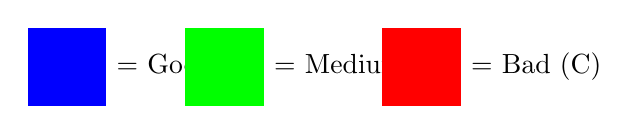
\begin{tikzpicture}
\node[inner sep=0pt] (r) at (0,0) {\tikz\fill[blue] (0,0) rectangle (\rectWidth,\rectHeight);};
\node[anchor=west] at (r.east) { = Good (A)};

\node[inner sep=0pt] (g) at (2,0) {\tikz\fill[green] (0,0) rectangle (\rectWidth,\rectHeight);};
\node[anchor=west] at (g.east) { = Medium (B)};

\node[inner sep=0pt] (b) at (4.5,0) {\tikz\fill[red] (0,0) rectangle (\rectWidth,\rectHeight);};
\node[anchor=west] at (b.east) { = Bad (C)};
\end{tikzpicture}
\vspace{2mm}

\caption{The poem orders obtained in Experiments 1 and 2 on all criteria, where every poem is colour coded with its ground truth category.The lower part of the table presents for comparison the orderings by human non-expert judges from \citet{lamb2015human}.}
\label{fig:ordering_all4_human}
\end{figure*}


\begin{table*}[ht]
\begin{center}
\small
\setlength{\tabcolsep}{4pt}
{
\begin{tabular}{ l|c|c|c|c|l }
\hline
\textbf{Criterion}& \textbf{Good} & \textbf{Medium} & \textbf{Bad} & \textbf{F-value} &\textbf{p-value} \\
\hline
 & \multicolumn{5}{c}{\textbf{GPT-4o 15}} \\
\hline
Average Innovativeness Score & 3.49 & 3.12 & 1.64 & 82.72 & 7.5e-21 \\
Average Quality Score & 3.48 & 2.98 & 1.71 & 92.31  & 3.1e-22 \\
Average Creativity Score & 3.46 & 3.15 & 1.77 & 78.8 & 2.96e-20\\
Average Poeticness Score & 3.82 & 3.42 & 2.15 & 60.27 & 3.75e-17 \\
Average Similarity Score & 3.41 & 2.86 & 2.13 & 49.28 & 4.9e-15 \\
\hline
 & \multicolumn{5}{c}{\textbf{GPT-4o 15n}} \\
\hline
Average Innovativeness Score & 10.99 & 9.57 & 3.63 & 108.06 & 2.62e-24 \\
Average Quality Score & 11.32 & 9.30 & 3.50 & 157.45  & 1.23e-29 \\
Average Creativity Score & 10.81 & 9.63 & 3.79 & 96.72 & 7.73e-23\\
Average Poeticness Score & 10.72 & 9.11 & 4.14 & 71.43 & 4.42e-19 \\
Average Similarity Score & 10.35 & 8.29 & 5.28 & 57.56 & 1.19e-16 \\
\hline
 & \multicolumn{5}{c}{\textbf{Claude-3-Opus 15}} \\
\hline
Average Innovativeness Score & 3.24 & 2.77 & 1.54 & 36.3 & 3.44e-12 \\
Average Quality Score & 3.52 & 2.84 & 1.43 & 94.47  & 1.56e-22 \\
Average Creativity Score & 3.49 & 2.93 & 1.64 & 50.04 & 3.43e-15\\
Average Poeticness Score & 3.85 & 3.2 & 1.8 & 72.02 & 3.53e-19 \\
Average Similarity Score & 3.37 & 2.69 & 1.58 & 90.5 & 5.55e-22 \\
\hline
 & \multicolumn{5}{c}{\textbf{Claude-3-Opus 15n}} \\
\hline
Average Innovativeness Score & 10.83 & 9.02 & 4.26 & 52.89 & 9.3e-16 \\
Average Quality Score & 11.65 & 9.06 & 3.33 & 132.23  & 4.2e-27 \\
Average Creativity Score & 11.11 & 8.95 & 4.02 & 62.55 & 1.46e-17\\
Average Poeticness Score & 11.42 & 8.81 & 3.79 & 85.15 & 3.27e-21 \\
Average Similarity Score & 11.22 & 8.63 & 4.13 & 111.08 & 1.11e-24 \\
\hline
 & \multicolumn{5}{c}{\textbf{Claude-3-Opus 90}} \\
\hline
Average Innovativeness Score & 3.04 & 2.82 & 2.26 & 30.09 & 1.96e-12 \\
Average Quality Score & 2.6 & 2.55 & 1.92 & 24.57  & 3.47e-9 \\
Average Creativity Score & 3.13 & 2.91 & 2.51 & 19.84 & 7.94e-8\\
Average Poeticness Score & 2.94 & 2.67 & 1.97 & 37.34 & 1.96e-12 \\
Average Similarity Score & 2.56 & 2.41 & 2.11 & 14.95 & 2.63e-6 \\
\hline
 & \multicolumn{5}{c}{\textbf{Claude-3-Opus 90n}} \\
\hline
Average Innovativeness Score & 56.5 & 48.9 & 31.1 & 41.2 & 2.64e-13 \\
Average Quality Score & 53.7 & 50.9 & 32.9 & 25.74  & 1.66e-9 \\
Average Creativity Score & 54.6 & 48.1 & 33.8 & 31.22 & 6.02e-11\\
Average Poeticness Score & 56.2 & 48.6 & 31.7 & 35.9 & 4.29e-12 \\
Average Similarity Score & 51.2 & 47.8 & 37.5 & 16.13 & 1.1e-6 \\

\end{tabular}
}
\end{center}
\caption{Average scores of poem evaluation in five criteria in Experiments 2 and 3.}\label{tbl:var_1_results_full}
\end{table*}



\begin{table*}[ht]
\begin{center}
\small
{
\begin{tabular}{ l|cccccl }
\hline
\textbf{Criterion}& \textbf{Description} \\
\hline
Typicality & How similar the poem is to other examples of poetry. \\
\hline
Quality & How good or high-quality the poem is as an example of poetry. \\
\hline
Wellbeing & How much the reader likes or enjoys the poem. \\
\hline
Effort  & How willing the reader is to spend time trying to understand the poem. \\
\hline
Skill  & How capable the author seems to be at writing poetry. \\
\hline
Imagination & How imaginative or creative the author of the poem appears to be. \\
\hline
Appreciation & How well the author seems to understand how poetry works. \\
\hline
Novelty & How different or unlike other poems the poem is. \\
\hline
Value  & How good or worthwhile the poem is considered to be. \\
\hline


\end{tabular}
}
\end{center}
\caption{Descriptions of the selected evaluation criteria by non-expert human judges presented in \citet{lamb2015human}}\label{tbl:original_criteria}
\end{table*}


\begin{table*}[h]
\centering
% \small
\begin{tabular}{|l|c|c|c|c|c|c|c|c|c|c|c|}
\hline
\multicolumn{12}{|c|}{\textbf{Claude-3-Opus 15n}} \\
\hline
\textbf{Poem ID} & \multicolumn{10}{c|}{\textbf{Scores}} & \textbf{Average Score} \\
\hline
Poem 27 & 14 & 15 & 15 & 14 & 15 & 15 & 14 & 15 & 15 & 14 & 14.6 \\
\hline
Poem 3 & 15 & 13 & 12 & 13 & 14 & 10 & 15 & 11 & 13 & 11 & 12.7 \\
\hline
Poem 7 & 13 & 14 & 9 & 11 & 13 & 14 & 13 & 14 & 14 & 12 & 12.7 \\
\hline
Poem 6 & 12 & 12 & 13 & 15 & 12 & 11 & 8 & 12 & 11 & 15 & 12.1 \\
\hline
Poem 8 & 11 & 9 & 14 & 10 & 10 & 13 & 7 & 13 & 12 & 8 & 10.7 \\
\hline
Poem 50 & 9 & 7 & 10 & 12 & 9 & 12 & 11 & 8 & 8 & 9 & 9.5 \\
\hline
Poem 54 & 7 & 11 & 7 & 6 & 11 & 9 & 12 & 9 & 9 & 13 & 9.4 \\
\hline
Poem 53 & 10 & 10 & 11 & 9 & 8 & 8 & 10 & 7 & 10 & 10 & 9.3 \\
\hline
Poem 41 & 8 & 8 & 8 & 8 & 7 & 7 & 6 & 10 & 7 & 6 & 7.5 \\
\hline
Poem 42 & 6 & 6 & 5 & 7 & 6 & 6 & 9 & 5 & 5 & 5 & 6.0 \\
\hline
Poem 61 & 5 & 5 & 6 & 5 & 5 & 5 & 5 & 6 & 6 & 7 & 5.5 \\
\hline
Poem 74 & 4 & 3 & 3 & 4 & 4 & 2 & 4 & 4 & 4 & 4 & 3.6 \\
\hline
Poem 79 & 3 & 2 & 2 & 3 & 3 & 1 & 3 & 2 & 3 & 1 & 2.3 \\
\hline
Poem 65 & 2 & 1 & 4 & 2 & 2 & 3 & 1 & 3 & 2 & 3 & 2.3 \\
\hline
Poem 69 & 1 & 4 & 1 & 1 & 1 & 4 & 2 & 1 & 1 & 2 & 1.8 \\
\hline
\multicolumn{12}{|c|}{\textbf{Claude-3-Opus 15}} \\
\hline
\textbf{Poem ID} & \multicolumn{10}{c|}{\textbf{Scores}} & \textbf{Average Score} \\
\hline
Poem 27 & 4 & 5 & 5 & 4 & 5 & 5 & 4 & 5 & 5 & 4 & 4.6 \\
\hline
Poem 3 & 5 & 3 & 4 & 4 & 4 & 3 & 5 & 3 & 4 & 3 & 3.8 \\
\hline
Poem 7 & 4 & 4 & 3 & 3 & 4 & 4 & 4 & 4 & 4 & 3 & 3.7 \\
\hline
Poem 6 & 3 & 2 & 4 & 5 & 3 & 3 & 3 & 3 & 3 & 5 & 3.4 \\
\hline
Poem 50 & 3 & 1 & 4 & 4 & 3 & 4 & 3 & 3 & 3 & 3 & 3.1 \\
\hline
Poem 53 & 3 & 1 & 4 & 3 & 3 & 3 & 3 & 3 & 3 & 3 & 2.9 \\
\hline
Poem 54 & 3 & 1 & 3 & 2 & 3 & 3 & 3 & 3 & 3 & 4 & 2.8 \\
\hline
Poem 8 & 3 & 1 & 4 & 3 & 3 & 4 & 2 & 3 & 3 & 2 & 2.8 \\
\hline
Poem 41 & 3 & 1 & 3 & 3 & 3 & 2 & 2 & 3 & 2 & 2 & 2.4 \\
\hline
Poem 42 & 2 & 1 & 2 & 2 & 2 & 2 & 3 & 3 & 2 & 2 & 2.1 \\
\hline
Poem 61 & 2 & 1 & 3 & 2 & 2 & 2 & 2 & 3 & 2 & 2 & 2.1 \\
\hline
Poem 74 & 2 & 1 & 2 & 2 & 2 & 2 & 2 & 2 & 2 & 2 & 1.9 \\
\hline
Poem 65 & 2 & 1 & 2 & 1 & 2 & 2 & 1 & 2 & 1 & 1 & 1.5 \\
\hline
Poem 79 & 2 & 1 & 2 & 1 & 2 & 1 & 1 & 2 & 1 & 1 & 1.4 \\
\hline
Poem 69 & 1 & 1 & 1 & 1 & 1 & 2 & 1 & 1 & 1 & 1 & 1.1 \\
\hline

\end{tabular}
\caption{Example of 10 evaluations of the same subset of 15 poems in Experiment 4 with Claude-3-Opus 15n and Claude-3-Opus, evaluating the criterion ``Creativity''. Poem's numbers indicate the categories they belong to: 1-30 ``Good'', 31-60 ``Medium'', 61-90 ``Bad''. These results confirm that the temperature parameter successfully randomises the output of its LMM, but our ICC results in the main body of the paper (and in Table.~\ref{tab:ICC_full}) show that those randomised outputs are consistent and reliable on average.}
\label{tab:poetry_scores_example_iccc}
\end{table*}

\begin{table*}[ht]
\centering
\small
\setlength{\tabcolsep}{4pt}
\begin{tabular}{l|l|l|l||l|l|l||l|l|l||l|l||l}
 & \multicolumn{3}{c|}{\textbf{Claude-3-Opus}}  & \multicolumn{3}{c|}{\textbf{Claude-3-Opus 15n}} & \multicolumn{3}{c||}{\textbf{GPT-4o}} & \multicolumn{3}{c}{\textbf{GPT-4o 15n}} \\
\hline
Type & ICC  & F & p-value & ICC  & F & p-value & ICC  & F & p-value & ICC  & F & p-value \\
\hline
& \multicolumn{12}{c}{\textbf{CREATIVITY}} \\
\hline
ICC1 & 0.84 & 54.66 & 1.63e-48 & 0.89 & 80.84 & 2.12e-58 & 0.78 & 36.25 & 8.17e-39 & 0.9 & 92.32 & 7.22e-62 \\
ICC2 & 0.84 & 53.59 & 4.14e-46 & 0.89 & 75.45 & 3.4e-54 & 0.78 & 42.59 & 6.54e-41 & 0.9 & 86.17 & 1.98e-57 \\
ICC3 & 0.84 & 53.59 & 4.14e-46 & 0.88 & 75.45 & 3.4e-54 & 0.81 & 42.59 & 6.54e-41 & 0.89 & 86.17 & 1.98e-57 \\
ICC1k & 0.98 & 54.66 & 1.63e-48 & 0.99 & 80.84 & 2.12e-58 & 0.97 & 36.25 & 8.17e-39 & 0.99 & 92.32 & 7.22e-62 \\
ICC2k & 0.98 & 53.59 & 4.14e-46 & 0.99 & 75.45 & 3.4e-54 & 0.97 & 42.59 & 6.54e-41 & 0.99 & 86.17 & 1.98e-57 \\
ICC3k & 0.98 & 53.59 & 4.14e-46 & 0.99 & 75.45 & 3.4e-54 & 0.98 & 42.59 & 6.54e-41 & 0.99 & 86.17 & 1.98e-57 \\
\hline
 & \multicolumn{12}{c}{\textbf{INNOVATIVE}} \\
 \hline
ICC1 & 0.91 & 101.03 & 2.99e-64 & 0.94 & 161.46 & 6.16e-77 & 0.81 & 44.61 & 1.28e-43 & 0.88 & 75.05 & 1.75e-56 \\
ICC2 & 0.91 & 105.98 & 1.47e-62 & 0.94 & 150.7 & 1.74e-71 & 0.81 & 51.25 & 4.41e-45 & 0.88 & 70.05 & 2.09e-52 \\
ICC3 & 0.91 & 105.98 & 1.47e-62 & 0.94 & 150.7 & 1.74e-71 & 0.83 & 51.25 & 4.41e-45 & 0.87 & 70.05 & 2.09e-52 \\
ICC1k & 0.99 & 101.03 & 2.99e-64 & 0.99 & 161.46 & 6.16e-77 & 0.98 & 44.61 & 1.28e-43 & 0.99 & 75.05 & 1.75e-56 \\
ICC2k & 0.99 & 105.98 & 1.47e-62 & 0.99 & 150.7 & 1.74e-71 & 0.98 & 51.25 & 4.41e-45 & 0.99 & 70.05 & 2.09e-52 \\
ICC3k & 0.99 & 105.98 & 1.47e-62 & 0.99 & 150.7 & 1.74e-71 & 0.98 & 51.25 & 4.41e-45 & 0.99 & 70.05 & 2.09e-52 \\
\hline
 & \multicolumn{12}{c}{\textbf{POETICNESS}} \\
 \hline
ICC1 & 0.91 & 98.95 & 1.07e-63 & 0.94 & 147.33 & 2e-74 & 0.81 & 43.34 & 6.179e-43 & 0.9 & 94.85 & 1.4e-62 \\
ICC2 & 0.91 & 102.67 & 9.13e-62 & 0.94 & 137.51 & 3.83e-69 & 0.81 & 49.62 & 2.4e-44 & 0.9 & 88.52 & 4.31e-58 \\
ICC3 & 0.91 & 102.67 & 9.13e-62 & 0.93 & 137.51 & 3.83e-69 & 0.83 & 49.62 & 2.4e-44 & 0.9 & 88.52 & 4.31e-58 \\
ICC1k & 0.99 & 98.95 & 1.07e-63 & 0.99 & 147.33 & 2e-74 & 0.98 & 43.34 & 6.17e-43 & 0.99 & 94.85 & 1.4e-62 \\
ICC2k & 0.99 & 102.67 & 9.13e-62 & 0.99 & 137.51 & 3.83e-69 & 0.98 & 49.62 & 2.4e-44 & 0.99 & 88.52 & 4.31e-58 \\
ICC3k & 0.99 & 102.67 & 9.13e-62 & 0.99 & 137.51 & 3.83e-69 & 0.98 & 49.62 & 2.4e-44 & 0.99 & 88.52 & 4.31e-58 \\
\hline
 & \multicolumn{12}{c}{\textbf{QUALITY}} \\
 \hline
ICC1 & 0.9 & 93.41 & 3.56e-62 & 0.94 & 156.2 & 5e-76 & 0.67 & 21.74 & 5.24e-28 & 0.89 & 83.52 & 3e-59 \\
ICC2 & 0.9 & 98.77 & 8.39e-61 & 0.94 & 145.79 & 1.23e-70 & 0.68 & 29.67 & 3.28e-33 & 0.89 & 77.96 & 5.5e-55 \\
ICC3 & 0.91 & 98.77 & 8.39e-61 & 0.94 & 145.79 & 1.23e-70 & 0.74 & 29.67 & 3.28e-33 & 0.88 & 77.96 & 5.5e-55 \\
ICC1k & 0.99 & 93.41 & 3.56e-62 & 0.99 & 156.2 & 5e-76 & 0.95 & 21.74 & 5.24e-28 & 0.99 & 83.52 & 3e-59 \\
ICC2k & 0.99 & 98.77 & 8.39e-61 & 0.99 & 145.79 & 1.23e-70 & 0.95 & 29.67 & 3.28e-33 & 0.99 & 77.96 & 5.5e-55 \\
ICC3k & 0.99 & 98.77 & 8.39e-61 & 0.99 & 145.79 & 1.23e-70 & 0.97 & 29.67 & 3.28e-33 & 0.99 & 77.96 & 5.5e-55 \\
\hline
 & \multicolumn{12}{c}{\textbf{SIMILARITY}} \\
 \hline
ICC1 & 0.59 & 15.46 & 9.2e-22 & 0.71 & 25.74 & 2.1e-31 & 0.48 & 10.37 & 1.46e-15 & 0.53 & 12.06 & 9.27e-18 \\
ICC2 & 0.59 & 15.66 & 2.2e-21 & 0.71 & 24.03 & 4.93e-29 & 0.48 & 9.9 & 1.35e-14 & 0.52 & 11.26 & 2.42e-16 \\
ICC3 & 0.59 & 15.66 & 2.2e-21 & 0.7 & 24.03 & 4.93e-29 & 0.47 & 9.9 & 1.35e-14 & 0.51 & 11.26 & 2.42e-16 \\
ICC1k & 0.94 & 15.46 & 9.2e-22 & 0.96 & 25.74 & 2.1e-31 & 0.9 & 10.37 & 1.46e-15 & 0.92 & 12.06 & 9.27e-18 \\
ICC2k & 0.94 & 15.66 & 2.2e-21 & 0.96 & 24.03 & 4.93e-29 & 0.9 & 9.9 & 1.35e-14 & 0.92 & 11.26 & 2.42e-16 \\
ICC3k & 0.94 & 15.66 & 2.2e-21 & 0.96 & 24.03 & 4.93e-29 & 0.9 & 9.9 & 1.35e-14 & 0.91 & 11.26 & 2.42e-16 \\
\hline
\end{tabular}
\caption{Results of ICC evaluations in Experiment 4, computed for both models with both scoring approaches and for the five criteria.}
\label{tab:ICC_full}
\end{table*}


\end{document}
